\documentclass[thesis]{thesis-gwu}

% this package is only used to generate some random text. 
% it is not needed in a true document
\usepackage{lipsum}
\graphicspath{{../../Fig/}}

% !TEX root = ../thesis-sample.tex

% --------- FRONT MATTER PAGES ---------------------
% Title of the thesis
\title{Multi-Robot Probabilistic Mapping and Exploration}

% Author name
\author{Evan Kaufman}

% Previous degrees
\bsdepartment{Mechanical Engineering}
\bsschool{Bucknell University}
\bsgrad{May 2012}

\hidemsdegree


\showcommitteepage % hide this page if you're doing a MS thesis
%\hidecommitteepage 
\committee{ %
Taeyoung Lee\\
Department of Mechanical and Aerospace Engineering\\
The George Washington University\\ 
Dissertation Director\\ % remember to add a space between committee members

Robert Pless\\
Department of Computer Science\\
The George Washington University\\
Committee Member\\

James Hahn\\
Department of Computer Science\\
The George Washington University\\
Committee Member\\

Chung Hyuk Park\\
Department of Biomedical Engineering\\
The George Washington University\\ 
Committee Member\\

Zhuming Ai\\
Information Management and Decision Architectures\\
U.S. Naval Research Laboratory\\ 
Committee Member

}

% Chair must be entered separately for formatting reasons.
\chair{Tayeoung Lee}
\chairtitle{Associate Professor of Mechanical and Aerospace Engineering}
% Department
\department{Mechanical and Aerospace Engineering}

\phdgrad{July 13, 2018}
\defensedate{July 13, 2018}
% Year of completion for copyright page and perhaps other places
\year=2018

% Copyright page
%\copyrightholder{Someone else}

%% Dedication
%\dedication{ 
%Add here...
%%
%%This dissertation is dedicated to my parents, Elizabeth Kaufman and Stephen Kaufman, who have consistently supported me throughout my many years of education. And others...
%}

% Acknowledgments
\acknowledgments{
My academic career has certainly been a long and bumpy road, but I was never alone. I would like thank many people for their support throughout my life for pursuing difficult and interesting work.

First and foremost, I would like to thank my parents. When I was younger, I was not always a great student, but my parents believed in me. When I struggled, they helped every time. I figured that this is what all parents do, but later I realized how lucky I was. Looking back, my academic career not ending prematurely is largely thanks to my mother and father. They have loved me and supported my academic pursuits, and I am extremely grateful.

I would also like to thank all other parts of my family, including my fianc\'ee, brother, grandparents, aunts, uncles, cousins, and close friends. We make it a priority to come together and support each other, even when our careers differ greatly and our lives change unpredictably. Despite the long academic road, they provided consistent support and love.

Finally, I would like to thank my research advisor, Taeyoung Lee, for the excellent guidance over the last six years. Unlike many relationships between advisors and students, he has treated his students like colleagues rather than subordinates. This way, I could focus on completing my research objectives properly rather than trying to impress superior figure. Taeyoung Lee knew just what to say to push my research forward, even when my mind was going another direction. His positive influence over my research has been unparalleled, and I will continue using his valuable lessons.% in the years to come.

 I think that finding and pursuing a passion is something truly special. Even though I find great satisfaction in doing anything well, regardless of how simple or complicated the task, I find myself extremely fortunate to pursue endeavors that I actually find exciting and stimulating. With tremendous support around me, I begin a career in an amazing field and ready to take on future challenges.
}

% -----------------------------------------------------------------
% Typically only one of Preface/Foreward/Prologue would be in your thesis.
% To choose one simply delete the others and they will automatically dissappear

%% Preface
%\preface{
%Add here...
%%    This is the preface. 
%%    It's another front matter page that offers additional detail into your work.
%%    Typically, only one (preface OR prologue OR foreword) is used. 
%%    You can remove the other sections by deleting them inside \texttt{tex/frontmatter.tex} or using the appropriate show or hide commands.
%}

%\prologue{
%    This is the prologue. 
%    It's another front matter page that offers additional detail into your work.
%    Typically, only one (preface OR prologue OR foreword) is used. 
%    You can remove the other sections by deleting them inside \texttt{tex/frontmatter.tex} or using the appropriate show or hide commands.
%}
%
%\foreword[2]{
%    This is the foreword. 
%    It's another front matter page that offers additional detail into your work.
%    Typically, only one (preface OR prologue OR foreword) is used. 
%    You can remove the other sections by deleting them inside \texttt{tex/frontmatter.tex} or using the appropriate show or hide commands.
%}
% ----------------------------------------------------------------------

% commands to show or hide front matter pages

\showcopyright
\showabstract
\showcommitteepage
\hidededication
\showacknowledgments
\hidepreface
\hideprologue
\hideforeword

% ------------ TABLE OF CONTENTS ----------------------
% Commands to hide or show lists of figures, tables, etc.
\showlistoffigures
\showlistoftables
\hidenomenclature

% --------- ACRONYMS and SYMBOLS ------------------------------
% TODO Deprecate the entire acronym package and switch to glossaries

% You can either use the acronymn or glossaries package (both work)
% Definition of any abbreviations used.
\abbreviations{
    \acro{CRTBP}{Circular Restricted Three Body Problem}
    \acro{NSA}{National Security Agency}
    \acro{SSME}{Space Shuttle Main Engine}
}
% call an abbreviation using \ac{abbrev}

% symbols and acronyms only show up when used in the text
\symbols{
    \acro{J}{Moment of Inertia}
}       

% if you want acronymn (simpler) then change these to show
\hidelistofabbreviations
\hidelistofsymbols

% if you want glossaries (more powerful) then leave above as hide
% GLOSSARIES package options - automatically turns off front pages from acronym package

% acronymns and symbols are basically the same, but there are two provided 
% locations where they can show up
\setabbreviationstyle[acronym]{long-short}
\setabbreviationstyle[abbreviation]{long-short}
\makeglossaries
% you can hide/show the glossaries page
\showglossarieslistofabbreviations
\showglossarieslistofsymbols
\showglossariesglossaryofterms

% acronyms defined in glossaries
\newabbreviation{lidar}{LIDAR}{Light Detection and Ranging}
% defining abbreviations like this allows for autocompletion
\newglossaryentry{filo}{
    name={FILO},
    type=\glsxtrabbrvtype,
    description={first in last out},
    first={first in last out (FILO)}
}

% glossary entries
\newglossaryentry{linux}{
    name=Linux,
    description={is a generic term referring to the family of Unix-like computer operating systems that use the Linux kernel},
    plural=Linuces
}

\newglossaryentry{matrix}{
    name={matrix},
    plural={matrices},
    description={rectangular array of quantiities}
}

% symbols
\newglossaryentry{M}{
    type=symbols,
    name={\ensuremath{M}},
    sort=M,
    description={a \gls{matrix}}
}

\newglossaryentry{F}{
    type=symbols,
    name={\ensuremath{F}},
    sort=F,
    description={External Force}
}
% Some abstract text
\abstract{
This dissertation focusses on robotic mapping and exploration of uncertain environments. Computational algorithms are developed to provide important probability and uncertainty properties. These algorithms are designed for real-time implementation for robotic autonomy.

Probabilistic occupancy grid mapping is developed using Bayesian probability. A novel approach to this problem is explored, which uses important physical properties of the environment and stochastic properties of depth sensors. We develop an exact solution to occupancy grid probability that can be achieved in real-time using sensor properties and conventional assumptions of an occupancy grid. The rapid computation allows the algorithm to consider large scans of measurements in 2D and 3D environments. The mapping algorithm is demonstrated with several numerical examples and experiments.

The next topic this dissertation addresses is autonomous exploration, where a robot selects actions to maximize its knowledge about the probabilistic map. We select Shannon's entropy as a metric that represents grid cell uncertainty. Using the earlier contributions on probabilistic occupancy grid mapping, we determine the expected value of entropy change from possible future measurements. This entropy change provides important insights for where a robot should move to maximize its mapping information gain. Dijkstra's search is integral to the algorithm to account for collision-free distances during motion planning. This algorithm is designed for 2D and 3D, where computation time is carefully considered to ensure real-time algorithm performance. Several versions of the exploration algorithm are applied to simulations and experiments.

The final topic of this dissertation relates to multi-vehicle cooperative scenarios. The mapping algorithm is multi-threaded to accept measurements from multiple sources with differing sensor properties. More importantly, the exploration algorithm structure is modified with a bidding-based framework. A series of auctions determines where robots should travel such that the members act together as a team. This solution is further extended to multi-vehicle patrol, where robots begin with an uncertain map, autonomously explore the space, and periodically revisit regions. Autonomous multi-vehicle patrol is accomplished through map degradation, where the probabilistic map becomes more uncertain over time, and the robots must revisit these spaces. These complex algorithms are demonstrated with numerical simulations.

In short, this dissertation proposes novel solutions to probabilistic occupancy grid mapping, autonomous exploration, and patrol in single-vehicle and multi-vehicle scenarios. Real-time implementation is paramount to ensure autonomy during a task. The efficacy of the approaches are shown with several experiments and numerical examples. 

}









%% DOCUMENT AREA
\begin{document}

%% !TEX root = ../thesis-sample.tex


\chapter{Introduction} \label{chap:intro}

This dissertation explores three key aspects of mobile robotics: occupancy grid mapping, autonomous exploration, and cooperation among robot teams. Several novel contributions are presented on these topics for complex and dynamic situations.


\section{Motivation and Goals}

The study of robotics has expanded tremendously in recent years as robots have replaced humans for dangerous, difficult, and repetitive tasks. Certain objectives, such as search-and-rescue, surveillance, and cleaning, require some level of autonomy, particularly with mobile robots exploring new and uncertain environments. While these tasks provide significant value to our society, they present nontrivial challenges for the robots, particularly in mapping, exploration, and cooperation.


\subsection{Building Probabilistic Maps}

The first topic this dissertation addresses is building accurate probabilistic maps, known as \emph{mapping}. Map generation is crucial for simultaneous localization and mapping (SLAM) because maps provide important information for the robot to determine its pose (localization), which includes its position and attitude. Mapping is also an integral part of vital mobile robot objectives, such as collision avoidance and trajectory planning. In short, mapping is of fundamental importance in mobile robotics.

Therefore, the map \emph{quality} deserves much attention. Robotics is inherently \emph{probabilistic}; no sensor reading or action from an actuator is deterministic. All robotic processes have some degree of uncertainty, and the mapping must account for this. Onboard sensors serve to improve the understanding of surrounding spaces, but the stochastic properties of those sensors must be reflected in the stochastic properties of the map. Therefore, we propose to develop a probabilistic map that accounts for the history of measurements and poses, and their associated stochastic properties. Here, each element of the map holds a probability based on measured data. In turn, this probability can be applied to tasks such as collision avoidance and predicting future map outcomes.


\subsection{Exploration in Uncertain Spaces}

The second topic of this dissertation focusses on the motions robots must choose to maximize their knowledge about the map while avoiding collisions, known as \emph{autonomous exploration}. Unlike conventional motion planning, where the map of the environment is assumed known, the robot must select motions with only the current knowledge of the environment. Therefore, real-time implementation of an active motion planning scheme is necessary while the probabilistic map is changing.

There are several important aspects to consider in autonomous exploration. Most importantly, the robot motion must be constrained to collision-free paths. The probabilistic map provides collision-free regions for this objective, and it also serves as a graph to determine an ordered set of collision-free waypoints. Additionally, the uncertainty of the map must be considered in the policy governing robotic motion. The method of decreasing map uncertainty can be computationally-expensive, so careful consideration with respect to algorithm complexity is vital. Furthermore, the efficiency of robot motions should be considered to avoid unnecessary travel distances. These objectives must all be achieved for an effective autonomous exploration policy.

%We proposed an autonomous exploration approach based on maximizing map information gain. Shannon's entropy serves as measure of map uncertainty to be minimized. This exploration scheme is formulated as a constrained optimization problem, where the robot predicts how much information will be acquired from various possible future actions, while also considering travel distance.

\subsection{Cooperation Among Autonomous Systems}

The final topic of this dissertation is cooperation among members of a robot team. All robots share the mutual objective of learning the map as quickly as possible. Each robot must select actions that consider the other team members. These considerations involve avoiding collisions among members, and avoiding actions that provide too much coverage of one region of the map while another region remains uncertain. Much like single-vehicle autonomous exploration, the multi-vehicle problem requires a computationally-inexpensive algorithm to handle numerous possible robot motions. These nontrivial goals can be handled by extending single-vehicle autonomous exploration with a bidding-based approach.

Multi-vehicle autonomous exploration can be extended further for surveillance purposes with autonomous patrol. The goal is to periodically capture many regions within a large space. Frequently, the robots are subject to dynamic obstacles (e.g. a walking person) or a changing environment (e.g. moving a chair), so the robots must account for these as well. Furthermore, an effective patrol policy can decrease the number of robots required to patrol an environment. The multi-vehicle autonomous exploration can be integrated with probabilistic map degradation to achieve autonomous patrol.

\section{Literature Review}

In this section, we discuss the existing approaches to occupancy grid mapping, autonomous exploration, and multi-vehicle cooperation. Several shortcomings with existing approaches are highlighted, which are addressed in the dissertation contributions.

\subsection{Occupancy Grid Mapping}

Here we describe the existing approaches to building probabilistic occupancy grid maps. Though several variations have been proposed, no approach uses the stochastic properties of depth sensors directly to obtain an exact Bayesian solution that can be computed in real-time.

\paragraph{Inverse Sensor Model} The key to generating a probabilistic occupancy grid map is known as the \emph{inverse sensor model}~\cite{ThrBurFox05}. The main idea is that a depth sensor has a probability density (e.g. Gaussian) that describes the stochastic properties of a sensor reading (e.g. a LIDAR range) with respect to the expected value of a reading (e.g. distance to a wall). This probability density is referred to as the \emph{forward sensor model}, as it relates a depth measurement conditioned on the occupancy of the map. 

In contrast, the inverse sensor model relates the occupancy of the map conditioned on the depth measurement. This problem is solved using Bayes' theorem. However, the occupancy grid map properties yield a complicated Bayesian probability; the computational cost has exponential complexity with respect to the number of grid cells captured within the depth sensor limits. It was previously-believed that this restriction makes solving the inverse sensor model in real-time impossible. This motivated approximate or estimated solutions, described next.

\paragraph{Approximated Function for the Inverse Sensor Model} Moravec and Elfes originally proposed a grid cell-based mapping for sonar sensors in~\cite{MorElf85}, and the probabilistic properties of the occupancy grid were formalized in~\cite{MorElf85,Elf89}. This approach models measurements with Gaussian probability density, although the occupancy of grid cells is not exactly known. Instead, the probability of grid cells are estimated with a Gaussian-like \emph{approximate function}. The authors show that occupancy probability converges to a final value following a Bayesian framework, though there is no conclusive proof that this probability is accurate. Nevertheless, this approach garnered much attention because it could efficiently produce robotic maps that nicely-resembled the occupancy of spaces around a robot.

Several other research studies have applied approximate functions in place of the inverse sensor model. For example, \cite{ChoLynHutKanBurKavThr05} proposed a simplified continuous function composed of lines patched together near a measurement reading. Furthermore, variations of approximate smoother functions in~\cite{Andert09,PirRutBisSch11,KhoElb12} contain Gaussian-like terms to apply occupancy grid mapping to 3D environments with more modern sensors. Numerous research studies have used the proposed approximate functions with questionable accuracy.

\paragraph{Learning the Inverse Sensor Model} The approximate nature of the inverse sensor model motivated a solution using machine learning. The main idea is to simulate maps, robot poses, and measurements with simulated noised based on the sensor stochastic properties. Then, an approximation the inverse sensor model is learned using an expectation maximization algorithm~\cite{Thr01,ThrBurFox05}. Unlike approximate functions based on intuition, the machine learning approach is based on the physical properties of sensors. However, this approach is undesirable in practice due to complexities associated to implementing a learning algorithm. For example, the accuracy of such inverse sensor models strongly depends on the samples selected for learning, but it is unclear how to select those samples, or how many samples are required to obtain a reasonable approximation. Furthermore, it is challenging to apply any learning algorithm over the large dimensional space composed of maps, poses, and measurements.

\paragraph{Log-Odds Ratio} Both approaches described above use the log-odds ratio to update grid cell probabilities. The log-odds ratio formulation is a popular framework for updating binary random variables with static state within a Bayesian filter. The main idea is that instead of multiplying terms from prior and current time steps, the properties of logarithms allow these terms to be simply added, while avoiding some truncation issues associated with probabilities close to $0$ or $1$~\cite{ThrBurFox05}. This approach is also popular because the inverse sensor model needs not consider prior probabilities. Instead, these approaches typically consider fixed uniform initial probabilities of all grid cells, which makes the formulation simpler.

However, the log-odds ratio formulation makes an assumption that is not consistent with the occupancy grid mapping problem. The approach yields a simplified solution by assuming that the probability of a measurement is independent of past measurements and robot poses. This assumption is frequently violated when past measurements and poses indicate the occupancy of other cells between the robot and the cell in question. As such, this approach neglects potentially important information when considering grid cell occupancy probability.

In short, other existing solutions to occupancy probability are inexact, and involve a potentially-harmful log-odds ratio assumption. These shortcomings motivate an exact solution to occupancy grid mapping that can be computed in real-time.

%It was previously-believed that the exact solution to occupancy grid mapping was impossible in real-time.



\subsection{Autonomous Exploration}

The next topic this dissertation addresses is autonomous exploration. The vast majority of work in simultaneous localization and mapping (SLAM) deals only with the aspect of estimating the environment and the poses of vehicles. These approaches are passive in the sense that SLAM is performed on incoming sensor measurements from vehicles following an arbitrary path. As such, human teleoperation and monitoring are often essential to guide the vehicles safely through unknown surroundings. Therefore, it is desirable that an active motion planning scheme is developed and integrated with SLAM such that vehicles are able to determine their path without human intervention, and explore unknown areas autonomously. The two approaches used to solve this problem are described next.

\paragraph{Frontier-Based Autonomous Exploration}

The most popular approach to solve the autonomous exploration problem is known as frontier-based exploration, originally-proposed in~\cite{Yam97,Yam98} for 2D applications, and was later extended to 3D with a visibility metric in~\cite{SawKriSri09} and~\cite{ZhuDinLinWu15,SenWan16,KleDor13} using the popular Octomap representation (a variation on occupancy grid mapping). The main idea is that robots toward the border between certain and uncertain space, referred to as a frontier. Then the robot takes depth measurement at this frontier, thus pushing back the boundary. This process is repeated until the map is well-known. Frontier-based exploration assumes that repeatedly moving toward the closest frontier and taking measurements are the best actions to gain new information about the map. However, these systematic actions, based on ad-hoc rules for what constitutes a frontier, do not consider the future uncertainty of the probabilistic map. Frontier-based approaches provide an intuitive solution, but lack optimality in map uncertainty or exploration time.

\paragraph{Entropy-Based Autonomous Exploration}
Entropy-based approaches address the suboptimal nature of frontier-based approaches by selecting robotic actions designed to decrease minimize map uncertainty~\cite{StaGriBur05,BurMooStaSch05}. These approaches use a measure of uncertainty known as Shannon's entropy, which becomes smaller as cell probabilities approach $0$ or $1$ (becoming more certain). Existing entropy-based approaches simulate possible future measurements from various locations with so-called ``hallucination measurements,'' which typically corresponds to expected depth measurements from the robot to the closest grid cell that is possibly occupied. Then, the robot analyzes how this measurement would affect the map uncertainty. However, this approach assumes that expected map entropy is equivalent to map entropy from expected measurements. This is not the case in general, however, as there is typically a nonzero probability that the hallucination measurement and true future measurement are not the same. Entropy-based approaches seek to optimize map uncertainty, but require large approximations which can decrease the accuracy of predictions.

In conclusion, existing autonomous exploration approaches are effective for eliminating the need for humans to control the robot. However, optimality remains quite difficult, so these approaches apply suboptimal or approximated solutions to achieve autonomous motions.


\subsection{Multi-Vehicle Cooperation}

The final topic relates to coordinating robotic efforts to build occupancy grid maps together. These concepts are further extended to autonomous cooperative patrol, where robots periodically revisit regions to monitor a large environment.

\paragraph{Cooperative Autonomous Exploration}

Multi-vehicle cooperation is essential for robots to explore large spaces autonomously so that robots coordinate their efforts to improve map information and avoid collisions. However, optimizing map coverage simultaneously from multiple vehicles becomes very complicated and computationally intractable. Instead, an auction-based approach addresses the computational restrictions effectively. Bidding-based approaches were introduced with~\cite{SimApfBurFoxMooThrYou00,DiaSte00}, and extended to several other robotic problems~\cite{GerMaj02,ZloSteDiaTha02,SarBal05,ChoBruHow09} exploring decentralization and task allocation with varying robot capabilities. In~\cite{SimApfBurFoxMooThrYou00}, a central executive assigns tasks to robots for maximizing overall utility of the group. This is accomplished by minimizing a coverage overlap among the members. Robots submit bids based on expected coverage of uncertain spaces and travel distance. The robot winning the auction is awarded the task, and the remaining bids are discounted to prevent robots from covering the same area, thereby coordinating the mapping efforts. Bidding-based approaches simplify multi-vehicle cooperation in a computationally-efficient manner, and integrate effectively with the autonomous mapping and exploration approaches proposed in this dissertation. 

\paragraph{Autonomous Patrol}

Robotic surveillance and cleaning are examples of tasks that require periodic observations of the same regions. Several patrolling approaches have been proposed in recent years to address this need. A popular approach is decomposing the reachable space into Voronoi diagrams~\cite{KolCar08,PorRoc10,PipChrWei13}. In~\cite{KolCar08}, edges between nodes of the Voronoi graph are heavily sensed to track intruders. In~\cite{PorRoc10}, regions of the Voronoi diagram are assigned to different robots, and issues with robots having underperforming surveillance capabilities are addressed in~\cite{PipChrWei13}. These approaches assume the map is well-known in advance, and require a Voronoi graph be generated from the map.

Other patrol approaches create new metrics about the environment. Cell periodicity is estimated in~\cite{KraFenCieDonDuc14,KraFenHanDuc16} by predicting and observing the long-term dynamics of objects at the same locations on an occupancy grid. This work is extended to exploring and navigating a human-populated environment for long-term autonomy. A bio-inspired approach is proposed in~\cite{ZhaXia11}, where robots cooperate by dropping digital pheromones based on the importance of events, where the pheromones weaken over time to prioritize future tasks. Another approach is formulating patrol as an optimization problem with respect to robot idleness in~\cite{YanZha16}. The prior work in autonomous patrol demonstrates that periodic actions can be incentivized with a metric to be optimized.


\section{Outline of Dissertation}

This dissertation is organized as follows. Chapter \ref{chap:pogm} introduces a novel approach to solve for the exact Bayesian probability of grid cells in real-time. Then, Chapter \ref{chap:ae2D} extends these contributions to autonomous exploration in 2D space, where a novel approach to predict future map uncertainty is presented. Next, Chapter \ref{chap:ae2D} applies the proposed occupancy grid mapping approach to 3D environments, and presents a method to simplify autonomous exploration in 3D environments with map projections. Chapter \ref{chap:multivehicle} applies this 3D mapping and exploration to multi-vehicle exploration and patrol scenarios using a bidding-based framework. Then, Chapter \ref{chap:ae3Dcomplex} extends exploration to complex 3D environments without 2D map projections. In these chapters, several numerical examples demonstrate the efficacies of the approaches. Furthermore, Chapter \ref{chap:Experiments} presents three experiments, which show the key contributions in this dissertation. Finally, these are followed by conclusions in Chapter \ref{chap:Conclusions}.

\section{Contributions}

There are three key contributions in this dissertation. The first two are novel solutions that find exact occupancy probabilities and predicted entropies, respectively. These contributions improve the quality and efficiency of autonomous mapping and exploration of uncertain environments for single-vehicle missions. The third contribution extends these concepts to multi-vehicle scenarios, where multiple members of a team work together to autonomously explore and patrol large environments.




\subsection{Summary of Contributions}

The first contribution is an exact Bayesian solution to occupancy grid mapping. The proposed approach considers that occupied spaces occlude measurement behind them, which allows certain mapping outcomes to be systematically grouped together. The exact solution to occupancy grid cell probability, which was previously-believed to have exponential complexity, is now possible to solve in real-time. Numerous numerical simulations and experiments demonstrate that the proposed mapping approach is effective and inexpensive in 2D and 3D scenarios.

% JINT17: This paper proposes a computationally efficient algo- rithm to construct the exact inverse sensor model. More explicitly, for a given forward sensor model defined by the probability distribution of range measurements, this algo- rithm yields the a posteriori probabilities of occupancy of all the cells within the area covered by the range sensor from the range measurements. The key idea is reducing the computational load by using the fact that if a cell is occu- pied, the occupancies of the other cells blocked by it is irrelevant to the forward sensor model, and this property is systematically utilized with various probabilistic prop- erties to derive a computationally-efficient solution to the inverse sensor model. Furthermore, the proposed approach integrates a priori probabilities of occupancy and multiple range measurements according to the Bayesian framework to obtain more accurate maps. As such, it contrasts from the existing framework based on log-odds ratios that impose an additional Markov assumption.


The second contribution is a new approach to autonomous exploration, where the robot predicts future occupancy grid map uncertainty, using a measure known as Shannon's entropy. This approach computes the expected values of grid cell entropies from potential future measurement rays with a novel approach to predict future measurement probabilities. These predictions are used to evaluate the benefit of possible robot actions to maximize map information gain. Then, we formulate autonomous exploration as an optimization problem to maximize an objective function that includes map uncertainty and travel costs. The probabilistic map is used for collision-avoidance and motion planning. These processes are designed for real-time applications, where the robot makes decisions as it learns information about the surrounding environment.

The final contribution coordinates the mapping and exploration efforts of multiple robots together. The mapping process is multi-threaded such that multiple members update the same occupancy grid. The exploration algorithm follows a bidding-based structure. Robots compete for tasks in a series of auctions, where the winning bid of one auction affects the bids of subsequent auctions, thereby coordinating the robot efforts. This cooperative approach is computationally-efficient in large environments, and follows a receding-horizon framework, such that map expected information gains are updated as quickly as possible. The proposed coordination is extended to autonomous patrol, where occupancy grid map probabilities are degraded over time, which promotes the robots to revisit areas periodically.

\subsection{List of Publications}

The following is a list of publications. These include research included in this dissertation, as well as contributions in control, data association, and estimation.

% TODO: update this list

\begin{itemize}
	\item E. Kaufman, K. Takami, Z. Ai, and T. Lee, ``Autonomous Quadrotor 3D Mapping and Exploration Using Exact Occupancy Probabilities,'' \textit{The Second IEEE International Conference on Robotic Computing}, Laguna Hills, January 2018, pp. 49--55.
	\item E. Kaufman, K. Takami, T. Lee, and Z. Ai, ``Autonomous Exploration with Exact Inverse Sensor Models,'' \textit{Journal of Intelligent }\&\textit{ Robotic Systems}, 2017, doi: 10.1007/s10846-017-0710-7.
	\item E. Kaufman, T. Lee, and Z. Ai, ``Autonomous Exploration by Expected Information Gain from Probabilistic Occupancy Grid Mapping,'' \textit{IEEE International Conference on Simulation, Modeling, and Programming for Autonomous Robots}, San Francisco, December 2016, pp. 246--251.
	\item E. Kaufman, T. Lee, Z. Ai, and I. S. Moskowitz, ``Bayesian Occupancy Grid Mapping via an Exact Inverse Sensor Model,'' \textit{Proceedings of the American Control Conference}, Boston, July 2016, pp. 5709-5715.
	\item E. Kaufman, T. A. Lovell, and T. Lee, ``Nonlinear Observability Measure for Relative Orbit Determination with Angles-Only Measurements,'' \textit{The Journal of the Astronautical Sciences}, 63(1): pp. 60-80, 2016, doi: 10.1007/s40295-015-0082-9.
	\item E. Kaufman, T. A. Lovell, and T. Lee, ``Minimum Uncertainty JPDA Filters and Coalescence Avoidance for Multiple Object Tracking,'' \textit{The Journal of the Astronautical Sciences}, 63(4): pp. 308-334, 2016, doi: 10.1007/s40295-016-0092-2.
	\item T. Wu, E. Kaufman, and T. Lee, ``Globally Asymptotically Stable Attitude Observer on SO(3),'' \textit{Proceedings of the 54th IEEE Conference on Decision and Control}, pp. 2164-2168, Osaka, Japan, December 2015.
	\item E. Kaufman, T. A. Lovell, and T. Lee, ``Nonlinear Observability Measure for Relative Orbit Determination with Angles-Only Measurements,'' \textit{Proceedings of the 25th AAS/AIAA Space Flight Mechanics Meeting}, Williamsburg, VA, Jan. 2015, AAS 15-451.
	\item E. Kaufman, T. A. Lovell, and T. Lee, ``Minimum Uncertainty JPDA Filter and Coalescence Avoidance Performance Evaluations,'' \textit{Proceedings of the 25th AAS/AIAA Space Flight Mechanics Meeting, Williamsburg}, VA, Jan. 2015, AAS 15-432.
	\item E. Kaufman, K. Caldwell, D. Lee, and T. Lee, ``Design and Development of a Free-Floating Hexrotor UAV for 6-DOF Maneuvers,'' \textit{Proceedings of the IEEE Aerospace Conference}, Mar. 2014, ASC 14-2527.
	\item E. Kaufman, T. A. Lovell, and T. Lee, ``Optimal Joint Probabilistic Data Association Filter Avoiding Coalescence in Close Proximity,'' \textit{Proceedings of the European Control Conference}, pp. 2709-2714, June 2014.
	\vspace*{0.5cm}
\end{itemize}










\chapter{Introduction} \label{chap:intro}

This dissertation explores three key aspects of mobile robotics: occupancy grid mapping, autonomous exploration, and cooperation among robot teams. Several novel contributions are presented on both related topics for complex and dynamic situations.


\section{Motivation and Goals}

The study of robotics has expanded tremendously in recent years as robots have taken on dangerous, difficult, and repetitive tasks instead of humans. Certain tasks, such as search-and-rescue, surveillance, and cleaning, require some level of autonomy, particularly with mobile robots exploring new and uncertain environments. While these tasks provide significant value to our society, they present nontrivial challenges for the robots, particularly in mapping, exploration, and cooperation.


\subsection{Building Probabilistic Maps}

The first topic this dissertation addresses is building accurate probabilistic maps, known as \emph{mapping}. Map generation is crucial for simultaneous localization and mapping (SLAM) because maps provide important information for the robot to determine its pose (localization), which includes its position and attitude. Mapping also provides knowledge for trajectory planning through an environment and collision avoidance with mapped obstacles. In short, mapping is of fundamental importance in mobile robotics.

Therefore, mapping quality deserves much attention. Robotics is inherently \emph{probabilistic}; no sensor reading or action from an actuator is deterministic. All robotic processes have some degree of uncertainty, and the mapping must account for this. Onboard sensors serve to improve the understanding of surrounding spaces, but the stochastic properties of those sensors must be reflected in the stochastic properties of the map. Therefore, we propose to develop probabilistic map that accounts for the history of measurements and poses, and their associated stochastic properties. Here, each element of the map holds a probability based on measured data. In turn, this probability can be applied to tasks such as collision-avoidance and predicting future map outcomes.


\subsection{Exploration in Uncertain Spaces}

The second topic of this dissertation focusses on the motions robots must choose to maximize their knowledge about the map while avoiding collisions, known as \emph{autonomous exploration}.

\subsection{Cooperation Among Autonomous Systems}

The final topic of this dissertation is cooperation among members of a robot team.

\section{Literature Review}

In this section, we discuss the existing approaches to occupancy grid mapping, autonomous exploration, and multi-vehicle cooperation. Several shortcomings with existing approaches are highlighted, which are addressed in the dissertation contributions.

\subsection{Occupancy Grid Mapping}




\subsection{Autonomous Exploration}

\subsection{Multi-Vehicle Cooperation}

\section{Outline of Dissertation}

ADD ONCE COMPLETE

\section{Contributions}




\subsection{Summary of Contributions}
\subsection{List of Publications}


% !TEX root = ../thesis-sample.tex

\chapter{Probabilistic Occupancy Grid Mapping} \label{chap:pogm}

In this chapter, we present the exact solution to occupancy grid map probability. This Bayesian approach uses the stochastic properties of sensors, and exploits important patterns in conditional probabilities. This solution is simulated in several examples to show the efficacy of the approach.

\section{Mapping Problem Definition}

Let a map $m$ be decomposed into $n_m$ evenly-spaced grid cells, where the $i$-th grid cell is assigned to a static binary random variable $\mathbf{m}_i$ for $i\in\braces{1,2,\ldots,n_m}$, that is defined as $\mathbf{m}_i=1$ when occupied, and $\mathbf{m}_i=0$ when free. The location and size of each grid cell is assumed known, where a smaller cell size (greater grid resolution) better represents a space, but increases computation and memory. Therefore, a map $m$ is defined by $\{\mathbf{m}_1,\ldots, \mathbf{m}_{n_m}\}$ ($2^{n_{m}}$ possible maps).

Another random variable is defined as $\bar{\mathbf{m}}_i=1-\mathbf{m}_i$ for convenience. The probability that the $i$-th cell is occupied is $P(\mathbf{m}_i)$, and the probability that it is free is $P(\bar{\mathbf{m}}_i)=1-P(\mathbf{m}_i)$. The random variables $\mathbf{m}_i$ are mutually independent, i.e.,
\begin{align}
P(m)=P(\mathbf{m}_1,\mathbf{m}_2,\ldots,\mathbf{m}_{n_m})=\prod_{i=1}^{n_m}P(\mathbf{m}_i).
\end{align}

Consider a range sensor that provides scans of the surrounding environment in order to identify the closest occupied space. The location and the direction of the sensor, referred to as the \emph{pose} at time $t$, is denoted by $X_t=(x_t,R_t)$. In a 2D environment, the planar position and direction of the robot at $t$ are denoted by $x_t\in\Re^2$ and $R_t\in\Sph^1=\braces{q\in\Re^2|\norm{q}=1}$, i.e., the attitude corresponds to a direction on a 2D plane. Similarly in a 3D environment, the spacial position and attitude are denoted by $x_t\in\Re^3$ and $R_t\in\SO=\braces{R\in\Re^{3\times3}|R^\T R=I,\det{R}=1}$. Let $X_{1:t}$ denote the history of poses from the initial time to the current time, i.e., $X_{1:t}=\{X_1,X_2,\ldots, X_t\}$. At each pose, the robot receives a 2D measurement \emph{scan}, composed of $n_z$ measurement \emph{rays}. These rays are 1D depth measurements of known direction from the current pose to the closest occupied space, subject to a known \emph{forward sensor model} $p(z_{t,l}|m,X_t)$, where $z_{t,l}$ is the $l$-th measurement ray of the $t$-th scan $Z_t=\braces{z_{t,1},z_{t,2},\ldots,z_{t,n_z}}$. The measurement history is denoted by $Z_{1:t}=\braces{Z_1,Z_2,\ldots,Z_t}$. 

The probability density function, namely $p(z_{t,l}|m,X_t)$ with respect to the depth of the $l$-th measurement ray conditioned on the map $m$ and the pose $X_t$ is commonly referred to as the \emph{forward sensor model}, which characterizes the corresponding depth sensor, such as the maximum range or accuracy. The forward sensor model satisfies (i) the ranges of all depth measurements are positive and finite, and (ii) a measurement cannot pass through occupied regions. Throughout this paper, we assume that the forward sensor model of the selected sensor is given. This can be determined empirically or analytically. For example, the \emph{beam model for range finders} satisfying  the above criteria is described in~\cite{ThrBurFox05}.

Occupancy grid mapping provides occupancy probabilities based on robot poses and measurement scans. The goal is to obtain $P(\mathbf{m}_i|X_{1:t},Z_{1:t})$, commonly referred to as the \emph{inverse sensor model} for a given forward sensor model $p(z_{t,l}|m,X_t)$ and the initial estimate of the map $P(m)$ with $X_{1:t}$ and $Z_{1:t}$.


\section{Inverse Sensor Model}

In this section, we propose an algorithm to compute the exact inverse sensor model efficiently. 
Suppose the probability of the map conditioned on the past poses and measurements, namely $P(m|X_{1:t-1},Z_{1:t-1})$, is known. Here we construct a posteriori probability $P(m|z_{t,l},X_{1:t},Z_{1:t-1})$, based on the current pose $X_t$, the measurement from the $l$-th ray $z_{t,l}$, and the given forward sensor model $p(z_{t_l}|m,X_t)$.



\subsection{Bayesian Framework}

The occupancy probability $P(m|z_{t,l},X_{1:t},Z_{1:t-1})$ is based on the forward sensor model $p(z_{t,l}|m,X_{1:t},Z_{1:t-1})$ that describe the distribution of the measurements for the given robot pose and the map. This specifies the stochastic characteristics of the sensor are a known distribution, specific to a particular depth sensor. One could certainly obtain a stochastic model by fitting a probability density to a controlled set of measurements. Bayes' rule yields
\begin{align}
\label{eqn:BayesRuleRayISM}
P(&m|z_{t,l},X_{1:t},Z_{1:t-1})%\nonumber\\&
=\frac{p(z_{t,l}|m,X_{1:t},Z_{1:t-1})P(m|X_{1:t-1},Z_{1:t-1})}{p(z_{t,l}|X_{1:t},Z_{1:t-1})},
\end{align}
where the second term in the numerator considers that $X_t$ carries no information about $m$ without $Z_t$.
If the current pose $X_t$ and map $m$ are known, then the measurement ray $z_{t,l}$ is independent of past poses $X_{1:t-1}$ and past measurements $Z_{1:t-1}$ to obtain
\begin{align}
P(m|z_{t,l},&X_{1:t},Z_{1:t-1})%\nonumber\\&
=\eta_{t,l}p(z_{t,l}|m,X_{t})P(m|X_{1:t-1},Z_{1:t-1}),
\end{align}
where the normalizing constant $\eta_{t,l}\in\Re$ absorbs all terms that do not depend on the map $m$.
Next, we compute the occupancy probability of each cell. Let $\mathcal{M}_i$ be the set of maps where the $i$-th cell is occupied, i.e., $\mathcal{M}_i =\{m\in\{0,1\}^{{n_m}}\,|\ \mathbf{m}_i=1\}$. To compute the probability of occupancy of the $i$-th cell, all possible combinations of map in $\mathcal{M}_i$ should be considered, i.e., 
\begin{align}
\label{eqn:InvSenModWithProbDens}
&P(\mathbf{m}_i|z_{t,l},X_{1:t},Z_{1:t-1})%\nonumber\\&
=\eta_{t,l}\sum_{m\in\mathcal{M}_i}p(z_{t,l}|m,X_{t})P(m|X_{1:t-1},Z_{1:t-1}).
\end{align}
Furthermore, to determine the normalizing constant $\eta_{t,l}$, the complement $\\P(\bar{\mathbf{m}}_i|z_{t,l},X_{1:t},Z_{1:t-1})$ must be calculated in the similar manner. Since there are $2^{n_{m}-1}$ maps in $\mathcal{M}_i$, these equations require $2^{n_m}$ terms to compute the summation for the $i$-th grid cell and normalizer, and this process should be repeated for all other cells along the measurement ray. This is the main reason why the existing results are based on approximations or learned solutions of the above expression. 

\subsection{Computationally-Efficient Solution}
% Include Fig 1 from JINT 2017

We propose a computational algorithm to evaluate \refeqn{InvSenModWithProbDens} efficiently~\cite{KauLeeAiMos16,KauTakAiLee17}. 
Since the cells outside of the sensor field of view (FOV) are not affected, we focus on a reduced map $r_l$ in the FOV of the $l$-th ray. This reduced map is chosen such that each cell of $r_l$ corresponds to a grid cell of map $m$ that the $l$-th ray intersects, ordered by increasing distance. Let $\mathbf{r}_{l,k}$ be the binary random variable representing the occupancy of the $k$-th cell of the $l$-th ray. The number of cells in the reduced map is denoted by $n_{r,l}\leq n_m$.

Next, let $\mathbf{r}_{l,k+}$ correspond to the event that the $k$-th cell of the $l$-th ray is occupied, cells with lower index (closer cells) are free, and cells with greater index (farther cells) may or may not be occupied, i.e., event $\mathbf{r}_{l,k+}$ occurs when \\$r\in\braces{r\in\{0,1\}^{{n_{r,l}}}\,|\mathbf{r}_{l,1}=0,\mathbf{r}_{l,2}=0,\ldots,\mathbf{r}_{l,k-1}=0,\mathbf{r}_{l,k}=1}$. Put differently, the $k$-th cell $\mathbf{r}_{l,k}$ is the closest occupied cell to current pose $X_t$ along the $l$-th ray. For example, see Figure \ref{fig:show_rkplus} that illustrates the event of $\mathbf{r}_{l,k+}$ when $l=1$ and $k=4$ for an one-dimensional cell array. This concept of grouping map outcomes can be easily extended to 2D using ray casting, where a 1D ray is spanning 2D space, which is easily determined from geometry, described in further detail in Section \ref{sec:RayCasting}. Then, the forward sensor model is identical for all maps defined by $\mathbf{r}_{l,k+}$, regardless of the occupancy of the cells beyond the $k$-th cell, and the corresponding forward sensor model $p(z_{t,l}|\mathbf{r}_{l,k+},X_{t})$ depends on the distance from $X_t$ to the $k$-th cell. Based on this, we present the mathematical expressions for the exact inverse sensor model, as summarized by \refeqn{RayISMAnswer} in Proposition \ref{prop:ISM}. Later in Section \ref{sec:RayScanComb}, these are also rearranged in computational algorithms. 



\begin{figure}
  \centering
  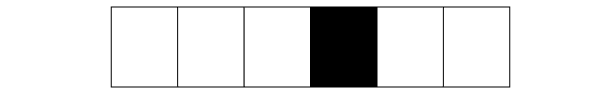
\includegraphics[width=0.4\textwidth]{rkplus_1.png}
    \centering
  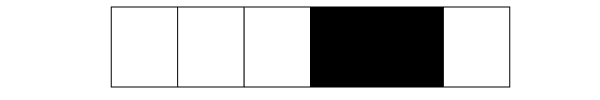
\includegraphics[width=0.4\textwidth]{rkplus_2.png}  
  \centering
  
\includegraphics[width=0.4\textwidth]{rkplus_3.png}
    \centering
  
\includegraphics[width=0.4\textwidth]{rkplus_4.png}
  \caption{Occupancy Grid Maps with Identical Forward Sensor Models}
  \medskip
  \small
  A robot located to the left of a 1D occupancy grid map $r_l$ composed of $n_{r,l}=6$ grid cells in four cases. In each case, cells the first three cells are free, the fourth cell is occupied, and the fifth and sixth cells may or may not be occupied. All above outcomes correspond to the event $\mathbf{r}_{l,4+}$.
  \label{fig:show_rkplus}
\end{figure}

\begin{prop}
\label{prop:ISM}
For the $l$-th measurement ray, the a posteriori probability of the occupancy of the $k$-th cell, namely the ray inverse sensor model, is given by
\begin{align}
\label{eqn:RayISMAnswer}
P(\mathbf{r}_{l,k}|z_{t,l},X_{1:t},Z_{1:t-1})&=\eta_{t,l}\tilde P(\mathbf{r}_{l,k}|z_{t,l},X_{1:t},Z_{1:t-1}),
\end{align}
where the unnormalized probability of the inverse sensor model is defined as
\begin{align}
\label{eqn:Unnormalized}
& \tilde P(\mathbf{r}_{l,k}|z_{t,l},X_{1:t},Z_{1:t-1})%\nonumber\\&
=P(\mathbf{r}_{l,k}|X_{1:t-1},Z_{1:t-1})\nonumber\\
&\quad\times 
\bigg[\sum_{i=1}^{k-1}\bigg\{\prod_{j=0}^{i-1}P(\bar{\mathbf{r}}_{l,j}|X_{1:t-1},Z_{1:t-1})\bigg\}%\nonumber\\
%&\quad\times 
p(z_{t,l}|\mathbf{r}_{l,i+},X_t)P(\mathbf{r}_{l,i}|X_{1:t-1},Z_{1:t-1})\bigg]\nonumber\\
&\quad + \bigg\{\prod_{j=0}^{k-1}P(\bar{\mathbf{r}}_{l,j}|X_{1:t-1},Z_{1:t-1})\bigg\}%\nonumber\\
%&\quad\times 
p(z_{t,l}|\mathbf{r}_{l,k+},X_t)P(\mathbf{r}_{l,k}|X_{1:t-1},Z_{1:t-1}),
\end{align}
where $P(\bar{\mathbf{r}}_{l,0}|X_{1:t-1},Z_{1:t-1})=P(\mathbf{r}_{l,n_r+1}|X_{1:t-1},Z_{1:t-1})=1$ is chosen for convenience and $p(z_{t,l}|\mathbf{r}_{l,(n_r+1)+},X_t)$ represents the probability density of the measurement when all of cells in the field of view of the $l$-th ray is not occupied. The normalizer $\eta_{t,l}$ is given by
\begin{align}
\label{eqn:allEta}
\eta_{t,l}
&=
\bigg[\sum_{i=1}^{n_{r,l}+1}\bigg\{\prod_{j=0}^{i-1}P(\bar{\mathbf{r}}_{l,j}|X_{1:t-1},Z_{1:t-1})\bigg\}p(z_{t,l}|\mathbf{r}_{l,i+},X_t)P(\mathbf{r}_{l,i}|X_{1:t-1},Z_{1:t-1})\bigg]^{-1},
\end{align}
and it is independent of the cell index $k$.
\end{prop}
\begin{proof}% TODO: add ref?
See Appendix A.
\end{proof}

%Note that the a priori estimate, $P(\mathbf{r}_{l,k}|X_{1:t-1},Z_{1:t-1})$ and its compliment $\\P(\bar{\mathbf{r}}_{l,k}|X_{1:t-1},Z_{1:t-1})=1-P(\mathbf{r}_{l,k}|X_{1:t-1},Z_{1:t-1})$ are available at the $t$-th step. Then, \refeqn{RayISMAnswer} yields a sequential occupancy grid mapping that can be applied whenever new measurements are available. 

%where a priori probability is $\mathbf{P}_k^-=P(\mathbf{r}_{k}|X_{1:t-1},Z_{1:t-1})$, its complement is $\bar{\mathbf{P}}_k^-=1-\mathbf{P}_k^-$, $P(\bar{\mathbf{r}}_{0}|X_{1:t-1},Z_{1:t-1})=P(\mathbf{r}_{n_{r,l}+1}|X_{1:t-1},Z_{1:t-1})=1$ for convenience, and $p(z_{t,l}|\mathbf{r}_{(n_{r,l}+1)+},X_t)$ represents the forward sensor model of a maximum sensor reading. 
%The proofs of \refeqn{RayISMAnswer}--\refeqn{Unnormalized} are given in~\cite{KauLeeAiMos16}. 

Since $\tilde P(\mathbf{r}_{l,k}|z_{t,l},X_{1:t},Z_{1:t-1})$ from \refeqn{Unnormalized} uses several repeated terms from the prior $\tilde P(\mathbf{r}_{l,k-1}|z_{t,l},X_{1:t},Z_{1:t-1})$, and $\eta_{t,l}$ is easily obtained from these as well, the computational cost of \refeqn{RayISMAnswer} is linear with respect to the number of cells along a measurement ray, amortized to $\mathcal{O}(1)$ for each cell. Because of this substantial computational improvement, the exact inverse sensor model can be applied in real-time. The process of updating each cell along a measurement ray is repeated for all rays composing scan $Z_t$.

% TODO: add update paragraph from JINT18

%Compared with \refeqn{InvSenModWithProbDens}, where the terms of the summation should be repeated $2^{n_{r,l}}$ times \emph{per each cell of the reduced map}, the proposed expressions \refeqn{RayISMAnswer} and \refeqn{allEta} are \textit{substantially} simpler. In fact, if \refeqn{Unnormalized} and \refeqn{allEta} are obtained recursively, requiring the summation of $O(n_{r,l}+1)$ rather than $O(n_{r,l}\times2^{n_{r,l}})$ as previously thought for \emph{all cells of the reduced map}, this yields an algorithm that is $\mathbf{n_{r,l}\times2^{n_{r,l}}/(n_{r,l}+1)}$ \textbf{times faster}.

\section{Mapping in 2D Space}

The above formulations describe how a single ray updates grid cells along its 1D path. Next we describe how measurement rays can update 2D maps, and how large scans of measurement rays are handled together.

% show RayCastingIllustration.png
\subsection{Ray Casting}
\label{sec:RayCasting}

Ray casting is the process of determining which cells a measurement ray might intersect, and the distances to these cells. The process is straightforward: follow a measurement unit vector from its minimum range $z_\text{min}$ to maximum range $z_\text{max}$, and identify the edges of all grid cells that it intersects. Save the cell index and Cartesian distance from the robot, and re-order the cells by increasing distance. An illustration of a simple example is shown in Figure \ref{fig:RayCastingIllustration}.

\begin{figure}[!ht]
    \centering
    \begin{subfigure}[t]{0.4\columnwidth}
        \centering
        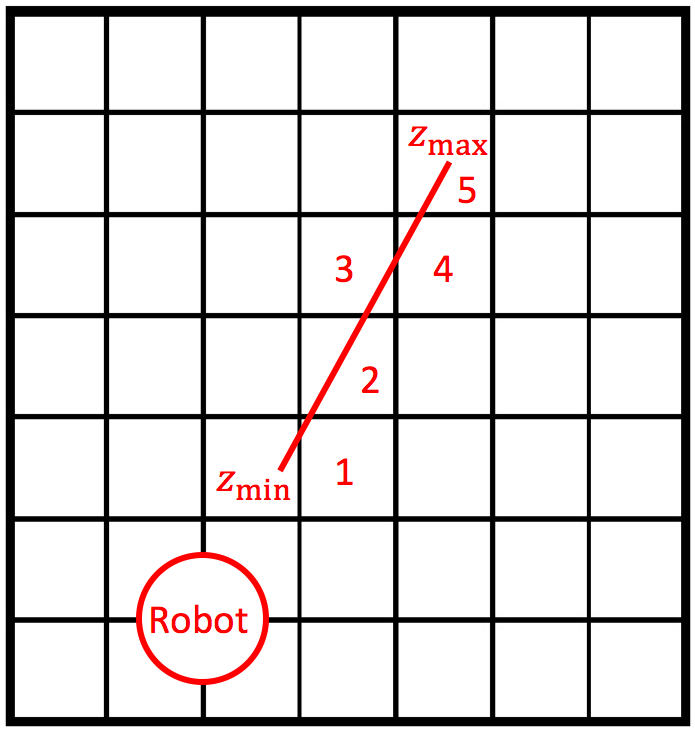
\includegraphics[width=\textwidth]{RayCastingIllustration.png}
        \caption{Ray Casting on a 2D Grid}
%        \label{fig:penn_map_total}
    \end{subfigure}
    \hspace*{0.05\columnwidth}
    \begin{subfigure}[t]{0.4\columnwidth}
        \centering
        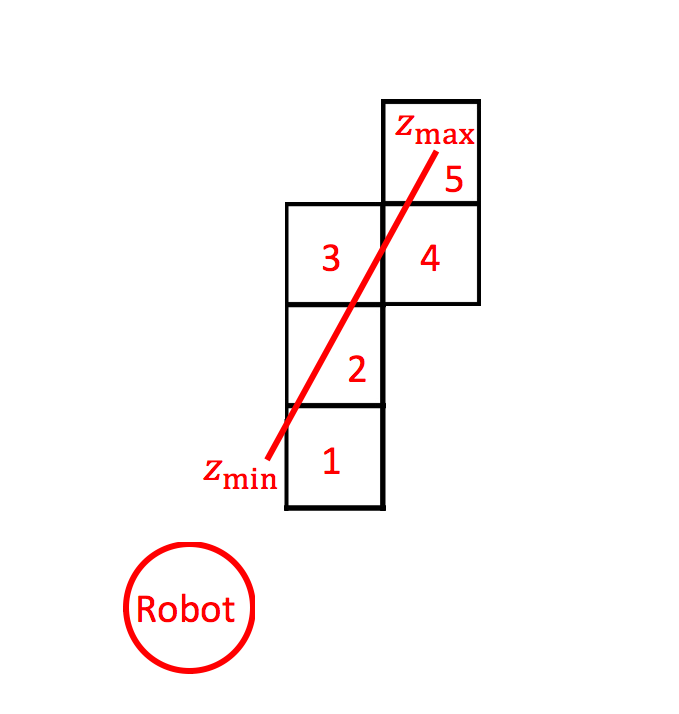
\includegraphics[width=\textwidth]{RayCastIllustrationReducedMapOnly.png}
        \caption{Reduced Map Only}
%        \label{fig:penn_map_zoom}
    \end{subfigure}
    \caption{Ray Casting Illustration}
    \label{fig:RayCastingIllustration}
    	\medskip
  	\small
	This simple 2D example illustrates how ray casting determines the cells that compose the reduced map for the inverse sensor model. The closest edges are used to determine which cells should be considered, and in what order. The complete map cell indices are temporarily saved as well, which are used to associate probabilities to cells of the reduced map.
\end{figure}

\subsection{Combining Measurements from a Single Scan}
\label{sec:RayScanComb}
Typically, many measurement rays are provided from a single scan from modern sensors.
Next, we describe two approaches to combine the inverse sensor models of numerous measurement rays.

\paragraph{Ray-By-Ray Approach}

At the $t$-th time step, consider the measurement scan $Z_t=\{z_{t,1},z_{t,2},...,z_{t,n_z}\}$. One may apply the results of Proposition \ref{prop:ISM} repeatedly for each ray to obtain a two-dimensional inverse sensor model because
\begin{align}
\label{eqn:RayByRayScanISM}
P(\mathbf{m}_i|X_{1:t},Z_{1:t})&%=P(\mathbf{m}_i|X_{1:t},Z_{1:t-1}|z_{t,1},z_{t,2},...,z_{t,n_z})\nonumber\\&
=P(\mathbf{m}_i|X_{1:t},Z_{1:t-1}|z_{t,1}|z_{t,2}|...|z_{t,n_z}).
\end{align}
In this approach, each ray is considered individually such that the inverse sensor model updates the probabilities of grid cells from one ray before subsequent rays of $Z_t$ are considered. Therefore, we assume the first measurement ray $z_{t,1}$ is independent of the remaining rays $z_{t,2:n_z}$. For the second ray, namely $z_{t,2}$, this may depend on $z_{t,1}$, but not subsequent rays $z_{t,3:n_z}$. By the time $z_{t,n_z}$ is considered, it may depend on all prior rays $z_{t,1:n_z-1}$. Therefore, the ray-by-ray approach considers rays within a single scan as partially dependent on each other.

In short, the proposed scan inverse sensor model is computed by \refeqn{RayISMAnswer}-\refeqn{RayByRayScanISM}. These are summarized in Algorithm \ref{alg:RayByRayISM} as a computationally efficient, recursive algorithm that avoids several repeated calculations of the same quantity. This algorithm utilizes temporary variables, where the required computational resources are minimized by computing the updated occupancy probabilities of all grid cells along a measurement ray together. Note that this function is only considering $l$-th ray at the $t$-th time step, where probabilities are subject to conditions on the history of poses $X_{1:t-1}$ and measurement scans $Z_{1:t-1}$, so these are removed from the algorithm for simplicity.

\vspace*{0.05\columnwidth}
\begin{algorithm}[H]
	Function: $P(m|X,Z)=\text{InverseSensorModelRayByRay}(P(m),X,Z)$\;
	% $\forall$ $l\in\braces{1,2,\ldots,n_{l}}$\;
	
	\For{$l=1,2,\ldots,n_{l}$}{
		Find $n_{r,l}$ cells from $m$ corresponding to $z_l$\;
		Initialize $\eta_l^{-1}=0$ and $P(\bar{\mathbf{r}}_{l,0}|X,z_{1:l-1})=1$ ($z_{1:0}$ is no condition)\;
		\For{$k=1,2,\ldots,n_{r,l}$}{
			$P(\mathbf{r}_{l,k+}|X,z_{1:l-1}) = P(\bar{\mathbf{r}}_{l,0:k-1}|X,z_{1:l-1})P(\mathbf{r}_{l,k}|X,z_{1:l-1})$\;
			$P(\bar{\mathbf{r}}_{l,0:k}|X,z_{1:l-1})=P(\bar{\mathbf{r}}_{l,0:k-1}|X,z_{1:l-1})(1-P(\mathbf{r}_{l,k}|X,z_{1:l-1}))$\;
    			$a_\text{temp}=P(\mathbf{r}_{l,k+}|X,z_{1:l-1})p(z_l|\mathbf{r}_{1:l,k+},X)$\;
   			$\tilde P(\mathbf{r}_{l,k}|X,z_{1:l})=P(\mathbf{r}_{l,k}|X,z_{1:l-1})\eta^{-1}_{l}+a_\text{temp}$\;
   			$\eta_l^{-1}=\eta_l^{-1}+a_\text{temp}$\;
		}
	$\eta_l^{-1}=\eta_l^{-1}+P(\bar{\mathbf{r}}_{l,0:n_{r,l}}|X,z_{1:l-1})p(z_\text{max})$\;
	$P(\mathbf{r}_{k}|z_{1:l})=\eta_l\tilde P(\mathbf{r}_{k}|X,z_{1:l})$ for all $k\in\braces{1,2,\ldots,n_{r,l}}$\;
	Substitute $P(\mathbf{r}_{k}|X,z_{1:l})$ back into $P(m|X,z_{1:l})$\;
	}
	Return $P(m|X,z_{1:n_{l}})=P(m|X,Z)$\;
\caption{Inverse Sensor Model of a Scan Updated Ray-By-Ray}
\label{alg:RayByRayISM}
\end{algorithm}
\vspace*{0.05\columnwidth}
\newpage





\paragraph{Synergistic Update Approach}

In this approach, all rays from a single scan are considered simultaneously for a synergistic update of all grid cells falling inside the scan FOV. However, the subsequent formulations require the assumption that all measurement rays within the scan are mutually independent, i.e.,
\begin{align*}
p(z_{t,1},z_{t,2},\ldots,z_{t,n_l}|\mathbf{m}_i,X_{1:t},Z_{1:t-1})=\prod_{l=1}^{n_l}p(z_{t,l}|\mathbf{m}_i,X_{1:t},Z_{1:t-1}).
\end{align*}
Here, we construct such two-dimensional inverse sensor model, referred to as the synergistic scan inverse sensor model.
Let $\mathcal L_i\subset\{1,\ldots, n_l\}$ be the set of rays that pass through the $i$-th cell, $\mathbf{m}_i$. Applying Bayes' rule repeatedly, we obtain
\begin{align}
P(\mathbf{m}_i|X_{1:t},Z_{1:t})
&=\tilde\zeta_i\braces{\prod_{l\in\mathcal{L}_i}p(z_{t,l}|\mathbf{m}_i,X_{1:t},Z_{1:t-1})}P(\mathbf{m}_i|X_{1:t-1},Z_{1:t-1})\nonumber\\
&=
\zeta_i P(\mathbf{m}_i|X_{1:t-1},Z_{1:t-1})%\nonumber\\&\quad\times
\prod_{l\in\mathcal{L}_i}\frac{P(\mathbf{m}_i|z_{t,l},X_{1:t},Z_{1:t-1})}{P(\mathbf{m}_i|X_{1:t-1},Z_{1:t-1})},
\label{eqn:ThirdBayesRule}
\end{align}
where $\tilde\zeta_i,\zeta_i\in\Re$ correspond to normalizing constants independent of $\mathbf{m}_i$. 

Suppose the $l$-th measurement ray intersects with the cell $\mathbf{m}_i$, and it is the $k$-th cell of the corresponding reduced map, i.e., $\mathbf{r}_{l,k}$ corresponds to the cell $\mathbf{m}_i$ in the $l$-th reduced map, and $\mathbf{r}_{l,k}=\mathbf{m}_i$ since they represent the same cell.  Then, we have $P(\mathbf{m}_i|z_{t,l},X_{1:t},Z_{1:t-1})=P(\mathbf{r}_{l,k}|z_{t,l},X_{1:t},Z_{1:t-1})=\eta_{t,l}\tilde P(\mathbf{r}_{l,k}|z_{t,l},X_{1:t},Z_{1:t-1})$. 

Using this, \refeqn{ThirdBayesRule} is rewritten as
\begin{align}
P(\mathbf{m}_i|X_{1:t},Z_{1:t})
&=\xi_i P(\mathbf{m}_i|{X_{1:t-1}},Z_{1:t-1})
\prod_{l\in\mathcal L_i}
\hat P(\mathbf{r}_{l,k}|z_{t,l},X_{1:t},Z_{1:t-1})
,
\label{eqn:ISM_Fusion}
\end{align}
where the normalizer $\xi_i$ is composed of the product of normalizers $\zeta_i$, and $\eta_i$. Here, we introduce a new term $\hat P(\mathbf{r}_{l,k}|z_{t,l},X_{1:t},Z_{1:t-1})$ for computational efficiency as
\begin{align}
&\hat P(\mathbf{r}_{l,k}|z_{t,l},X_{1:t},Z_{1:t-1})
\triangleq \frac{\tilde P(\mathbf{r}_{l,k}|z_{t,l},X_{1:t},Z_{1:t-1})}{P(\mathbf{m}_i|X_{1:t-1},Z_{1:t-1})}
\nonumber\\&=
\sum_{i=1}^{k-1}\bigg\{\prod_{j=0}^{i-1}P(\bar{\mathbf{r}}_{l,j}|X_{1:t-1},Z_{1:t-1})\bigg\}p(z_{t,l}|\mathbf{r}_{l,i+},X_t)P(\mathbf{r}_{l,i}|X_{1:t-1},Z_{1:t-1})
\nonumber\\&\quad
+
\bigg\{\prod_{j=0}^{k-1}P(\bar{\mathbf{r}}_{l,j}|X_{1:t-1},Z_{1:t-1})\bigg\}p(z_{t,l}|\mathbf{r}_{l,k+},X_t),
\end{align}
where we have used \refeqn{Unnormalized}. Similarly, its complement is
\begin{align}
P(\bar{\mathbf{m}}_i|{{X_{1:t}}},Z_{1:t})
&=\xi_i P(\bar{\mathbf{m}}_i|{X_{1:t-1}},Z_{1:t-1})
\prod_{l\in\mathcal L_i}
\hat P(\bar{\mathbf{r}}_{l,k}|z_{t,l},X_{1:t},Z_{1:t-1})
,
\label{eqn:ISM_Bar_Fusion}
\end{align}
where $\hat P(\bar{\mathbf{r}}_{l,k}|z_{t,l},X_{1:t},Z_{1:t-1})$ is defined as
\begin{align}
&\hat P(\bar{\mathbf{r}}_{l,k}|z_{t,l},X_{1:t},Z_{1:t-1})
\triangleq\frac{\tilde P(\bar{\mathbf{r}}_{l,k}|z_{t,l},X_{1:t},Z_{1:t-1})}{P(\bar{\mathbf{m}}_i|X_{1:t},Z_{1:t-1})}
\nonumber\\
&=\sum_{i=1}^{k-1}\bigg\{\prod_{j=0}^{i-1}P(\bar{\mathbf{r}}_{l,j}|X_{1:t-1},Z_{1:t-1})\bigg\} p(z_{t,l}|\mathbf{r}_{l,i+},X_t)P(\mathbf{r}_{l,i}|X_{1:t-1},Z_{1:t-1})
\nonumber
\\
&\quad
+\frac{
\sum_{i=k+1}^{n_{r,l}+1}\bigg\{\prod_{j=0}^{i-1}P(\bar{\mathbf{r}}_{l,j}|X_{1:t-1},Z_{1:t-1})\bigg\}p(z_{t,l}|\mathbf{r}_{l,i+},X_t)P(\mathbf{r}_{l,i}|X_{1:t-1},Z_{1:t-1})}{P(\bar{\mathbf{r}}_{l,k}|X_{1:t-1},Z_{1:t-1})},
\end{align}
which is obtained from \refeqn{tildePbar}. Since % TODO: ref in appendix
\begin{align*}
P(\mathbf{m}_i|X_{1:t},Z_{1:t})+P(\bar{\mathbf{m}}_i|X_{1:t},Z_{1:t})=1,
\end{align*}
the normalizer $\xi_i$ is obtained using \refeqn{ISM_Fusion} and \refeqn{ISM_Bar_Fusion} as,
\begin{align}
&\xi_i=
\bigg[
P(\mathbf{m}_i|{X_{1:t-1}},Z_{1:t-1})
\prod_{\mathcal L_i}
\hat P(\mathbf{r}_{l,k}|z_{t,l},{X_{1:t}},Z_{1:t-1})
\nonumber\\&\quad
+
P(\bar{\mathbf{m}}_i|{X_{1:t-1}},Z_{1:t-1})
\prod_{\mathcal L_i}
\hat P(\bar{\mathbf{r}}_{l,k}|z_{t,l},X_{1:t},Z_{1:t-1})
\bigg]^{-1},\label{eqn:xi}
\end{align}
which is substituted into \refeqn{ISM_Fusion} to obtain the complete scan inverse sensor model $P(\mathbf{m}_i|X_{1:t},Z_{1:t})$. 


The synergistic scan inverse sensor model algorithm is summarized with the pseudocode of Algorithm \ref{alg:SynergisticScanISM} as a computationally efficient, recursive algorithm that avoids repeated calculations of the same quantity. This algorithm utilizes the following temporary variables to develop the algorithm in an efficient recursive form, defined as
\begin{align*}
a_k&=\sum_{i=1}^{k-1}\bigg\{\prod_{j=0}^{i-1}P(\bar{\mathbf{r}}_{l,j}|X_{1:t-1},Z_{1:t-1})\bigg\}p(z_{t,l}|\mathbf{r}_{l,i},X_t)P(\mathbf{r}_{l,i}|X_{1:t-1},Z_{1:t-1}),
\\
b_k&=\prod_{j=0}^{k-1}P(\bar{\mathbf{r}}_{l,j}|X_{1:t-1},Z_{1:t-1}),
\nonumber\\
c_k&=\frac{
\sum_{i=k+1}^{n_{r,l}+1}\bigg\{\prod_{j=0}^{i-1}P(\bar{\mathbf{r}}_{l,j}|X_{1:t-1},Z_{1:t-1})\bigg\}p(z_{t,l}|\mathbf{r}_{l,i+},X_t)P(\mathbf{r}_{l,i}|X_{1:t-1},Z_{1:t-1})}{P(\bar{\mathbf{r}}_{l,k}|X_{1:t-1},Z_{1:t-1})},
\end{align*}
as well as $d$ and $e$ for the two terms composing \refeqn{xi}. Once again, the history of poses and measurement scans are removed from the pseudocode for simplicity.

% TODO: check spacing of algorithms once complete
\vspace*{0.05\columnwidth}
\begin{algorithm}[H]
	Function: $P(m|X,Z)=\text{InverseSensorModelSynergistic}(P(m),X,Z)$\;
	\For{$l=1,2,\ldots,n_{l}$}{
		Find $n_{r,l}$ cells from $m$ corresponding to $z_l$\;
		Define $P(\mathbf{r}_{l,0})=0$, $P(\bar{\mathbf{r}}_{l,0})=1$, $P(\mathbf{r}_{l,n_{r,l}+1})=1$, and $c_{n_{r,l}+1}=0$\;
		\For{$k=1,2,\ldots,n_{r,l}$}{
			\If{$k=1$}{
				$a_1=0$, $b_1=1$\;
			}
			\Else{
				$a_k=a_{k-1}+b_{k-1}p(z_{l}|\mathbf{r}_{l,k-1},X)P(\mathbf{r}_{l,k-1})$, $b_k=b_{k-1}P(\bar{\mathbf{r}}_{l,k-1})$\;
			}
		}
		\For{$k = n_{r,l},n_{r,l}-1,...,1$}{
			$c_k=\frac{P(\mathbf{r}_{l,k+1})}{P(\bar{\mathbf{r}}_{l,k})}c_{k+1}+b_{k}p(z_{t,l}|\mathbf{r}_{l,k+1},X)P(\mathbf{r}_{l,k+1})$\;
		}
		\For{$k = 1,2,...,n_{r,l}$}{
			$\hat P(\mathbf{r}_{l,k}|z_{t,l},X)=a_k+b_kp(z_{t,l}|\mathbf{r}_{l,k},X)$, $\hat P(\bar{\mathbf{r}}_{l,k}|z_{t,l},X,)=a_k+c_k$\;
		}
	}
	\For{$i\in m_\text{FOV}$ \text{(map cells inside FOV)}}{
		Obtain the set $\mathcal L_i$ of $l_i$ measurement rays intersecting this cell\;
		\If{$l_i>0$}{
			$d=P(\mathbf{m}_i)\prod_{\mathcal L_i}\hat P(\mathbf{r}_{l,k}|z_{t,l},X)$\;
			$e=P(\bar{\mathbf{m}}_i)\prod_{\mathcal L_i}\hat P(\bar{\mathbf{r}}_{l,k}|z_{t,l},X)$\;
			$P(\mathbf{m}_i|X,Z)=\frac{d}{d+e}$\;
		}
		\Else{
			$P(\mathbf{m}_i|X,Z)=P(\mathbf{m}_i)$\;
		}
	}
	Return $P(m|X,Z)$\;
\caption{Inverse Sensor Model of a Scan Updated Synergistically}
\label{alg:SynergisticScanISM}
\end{algorithm}
\vspace*{0.05\columnwidth}




In short, we propose two alternatives for combining inverse sensor models for multiple rays within a scan. The ray-by-ray approach updates the entire map one ray at a time with some dependancies among the rays, while the synergistic approach considers all rays together where rays are assumed mutually independent.


% TODO: move to 3D mapping part
%\subsection{Multi-Sensor Fusion}

% TODO: move to experiment part
%\subsection{Practical Implications}

\subsection{Numerical Examples}

In contrast to the current approximate inverse sensor models, the proposed ray-by-ray and synergistic algorithms evaluate the exact inverse sensor model efficiently without relying on approximations, learned solutions, or log-odds ratio assumptions. The following simulations show two examples comparing an approximate inverse sensor model with the proposed exact inverse sensor model, either with integrating multiple measurements ray-by-ray or synergistically. The proposed algorithms yield substantially more accurate maps for the same set of measurements.


\paragraph{Approximate Inverse Sensor Model}

We compare the proposed exact solution to the inverse sensor model with an approximate algorithm developed for a Microsoft Kinect sensor~\cite{PirRutBisSch11,KhoElb12}, summarized as follows. The probability that the $i$-th grid cell $\mathbf{m}_i$ is occupied conditioned on the measurement ray $z_{t,l}$ (the $l$-th ray at the $t$-th time step) at the pose $X_t$ is the continuous function
\begin{align}
\label{eqn:ISM_Approx_1}
P(\mathbf{m}_i|z_{t,l},X_t)=\begin{cases}
0.3+(\frac{k}{\sigma\sqrt{2\pi}}+0.2)e^{-\frac12\left(\frac{\hat z_{l,i}-z_{t,l}}{\sigma}\right)^2}\ &\text{if}\ z_{t,l}\leq \hat z_{l,i},
\\
0.5+\frac{k}{\sigma\sqrt{2\pi}}e^{-\frac12\left(\frac{\hat z_{l,i}-z_{t,l}}{\sigma}\right)^2}\ &\text{if}\ z_{t,l}>\hat z_{l,i},
\end{cases}
\end{align}
which is based on the expected distance to the cell $\hat z_{l,i}$ with parameters $k=\sigma=0.6$. This follows the structure of the approximate inverse sensor model proposed in~\cite{Andert09}. The main idea of this approach is that the probability of a cell being occupied (i) near a measurement is high (measurement likely hits this cell), (ii) between the robot and the measurement is low (measurement passes through these cells), and (iii) beyond the measurement is unchanged (the robot cannot measure through a wall/object). 

Then, these probabilities are combined in a weighted fashion such that all measurements rays of scan $Z_t$ simultaneously update the same grid cell in a log-odds format,
\begin{align}
\label{eqn:ISM_Approx_2}
\log\left(\frac{P(\mathbf{m}_i|Z_{t},X_t)}{1-P(\mathbf{m}_i|Z_{t},X_t)}\right)
=
\frac1{\sum_{z_{t,l}\in\mathbf{m}_i}\hat z_{l,i}}\sum_{z_{t,l}\in\mathbf{m}_i}\log\left(\frac{P(\mathbf{m}_i|z_{t,l},X_t)}{1-P(\mathbf{m}_i|z_{t,l},X_t)}\hat z_{l,i}\right).
\end{align}


\paragraph{Mapping a Hallway with the Ray-By-Ray Approach}

First, we compare the proposed exact solution to the ray-by-ray inverse sensor model summarized in Algorithm \ref{alg:RayByRayISM} with an approximations of \refeqn{ISM_Approx_1}--\refeqn{ISM_Approx_2}.
Table~\ref{tab:penn} shows the mapping parameters and data specifications for the actual odometry and lidar measurements from University of Pennsylvania through Coursera open course~\cite{coursera}. Among these parameters, cell resolution and the number of rays have the greatest impact on computation. In general, the finer the grid, the greater the memory and computational requirements are because the computational order of \refeqn{RayISMAnswer} grows linearly with the number of grid cells inside the sensor range limits. Since the inverse sensor models are combined sequentially as shown in \refeqn{RayByRayScanISM}, the number of rays considered are proportional to the computation order as well.
Figure~\ref{fig:penn_map} shows the direct comparison of the resulting map based on the approximate and proposed inverse sensor model.
As shown in the figure, both approaches capture the structure of the environment. However, the significant differences can be seen, particularly with an enlarged mapping section in Figure~\ref{fig:penn_map_zoom}.

To quantify the degree of map uncertainty, we define the entropy of the map as 
\begin{align*}
H(P(m|X_{1:t},Z_{1:t}))&=-\sum_{i=1}^n\big\{P(\mathbf{m}_i|X_{1:t},Z_{1:t})\log P(\mathbf{m}_i|X_{1:t},Z_{1:t})\nonumber\\
&\qquad+(1-P(\mathbf{m}_i|X_{1:t},Z_{1:t}))\log(1-P(\mathbf{m}_i|X_{1:t},Z_{1:t}))\big\},
\end{align*}
which is maximized when the probability of occupancy is $0.5$ for all cells (more uncertain), and it is minimized when they are either $0$ or $1$ (less uncertain). 
The entropy differences among the algorithms can be clearly depicted in Figure~\ref{fig:entropy_comp} at frame 2280.
The red part of the map shows the maximum  entropy whereas blue shows lowest entropy for the cell.
Finally, overall improvement was demonstrated in Figure~\ref{fig:entropy} resulting in an improved entropy value per grid cell throughout the mapping process.
In short, the proposed exact occupancy grid mapping produced a cleaner map with lower entropy from the same set of measurements.

\begin{center}
\captionof{table}{Experimental Parameters Provided from the Dataset}
\label{tab:penn}
    \begin{tabular}{r | c}
        Parameters & Value\\ \hline\hline
        Map dimension & 576x448 [pixel]\\
        Resolution & 1/16 [m]\\
        Scan angle & [-2.36, 2.36]\\
        Ray number & 1081\\
        Total frame & Every 120 scans out of 3701\\
    \end{tabular}
\end{center}

\begin{figure}[!ht]
    \centering
    \begin{subfigure}[t]{0.8\columnwidth}
        \centering
        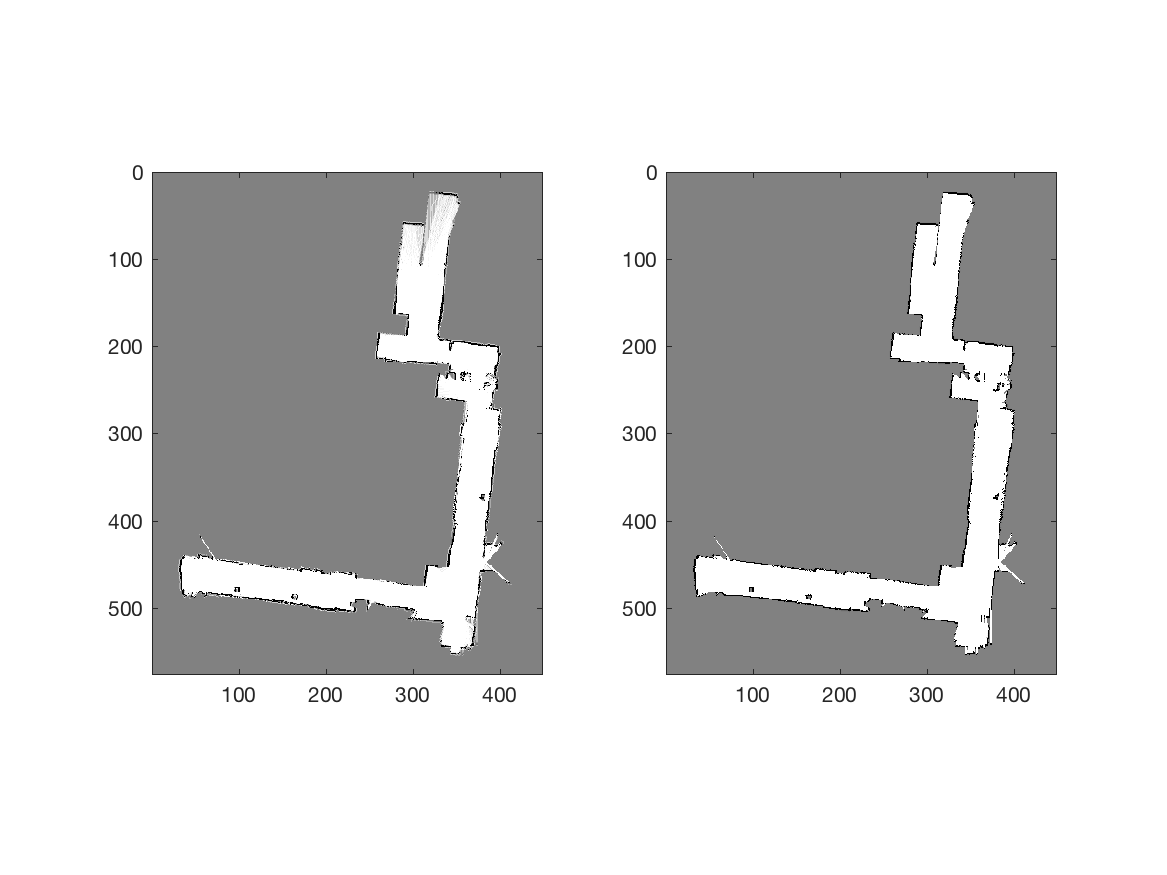
\includegraphics[trim={1.5cm 3.5cm 1.5cm 1.5cm},clip,width=\textwidth]{map_comparison.png}
        \caption{Comparison of the total mapped environment based on the approximate (left) and proposed (right) inverse sensor model.}
        \label{fig:penn_map_total}
    \end{subfigure}
    \begin{subfigure}[t]{0.8\columnwidth}
        \centering
        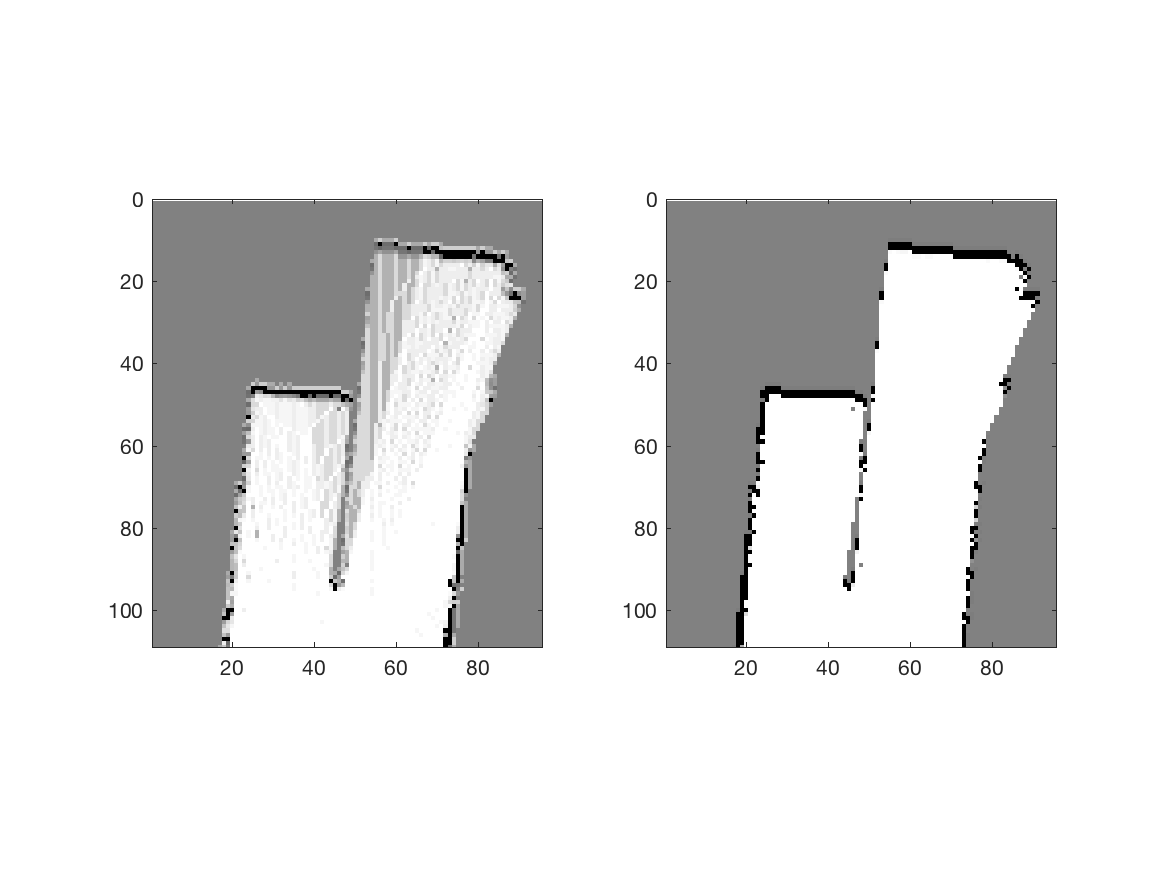
\includegraphics[trim={1.5cm 3.5cm 1.5cm 1.5cm},clip,width=\textwidth]{map_zoom.png}
        \caption{Evidence of significant improvement at certain area of the map.}
        \label{fig:penn_map_zoom}
    \end{subfigure}
    \caption{Comparison of Proposed Ray-By-Ray Approach with Approximate Solution}
	\medskip
	\small
	Using experimental sensor data, the map was generated using an approximate and the proposed exact inverse sensor models. The laser sensor and odometry data used for the experiment was provided by University of Pennsylvania open course robotics estimation and learning on Coursera~\cite{coursera}.
    \label{fig:penn_map}
\end{figure}


\begin{figure}[!ht]
    \centering
    \begin{subfigure}[t]{0.35\columnwidth}
        \centering
        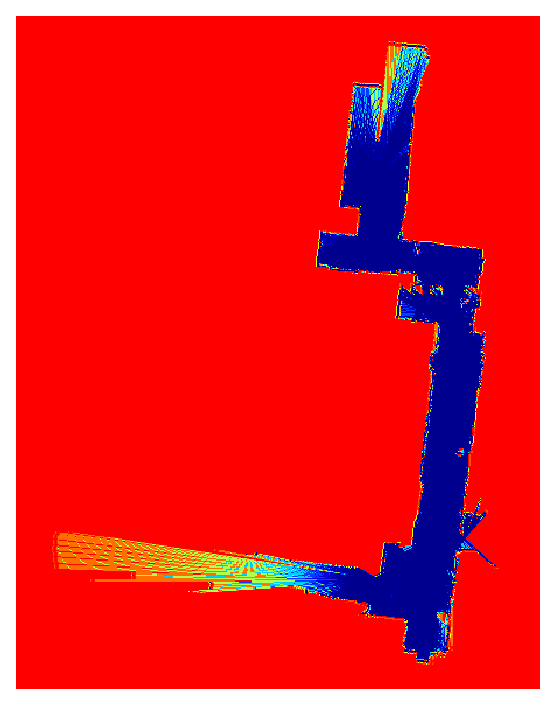
\includegraphics[width=\textwidth]{AISM_Image_inf_19.pdf}
        \caption{Approximate inverse sensor model}
        \label{fig:AISM}
    \end{subfigure}
    \begin{subfigure}[t]{0.35\columnwidth}
        \centering
        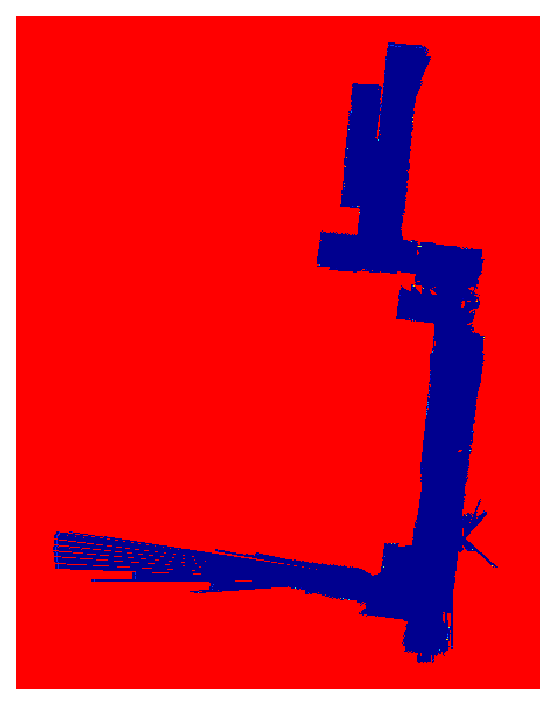
\includegraphics[width=\textwidth]{EISM_Image_inf_19.pdf}
        \caption{Exact inverse sensor model}
        \label{fig:EISM}
    \end{subfigure}
    \caption{Map Uncertainty Comparison Between Proposed Ray-By-Ray Approach and Approximate Solution}
	\medskip
	\small
	The entropy is compared between the approximate and proposed exact inverse sensor models at step 2280. The blue areas show the lowest entropy while red shows highest.
\label{fig:entropy_comp}
\end{figure}


\begin{figure}
  \centering
  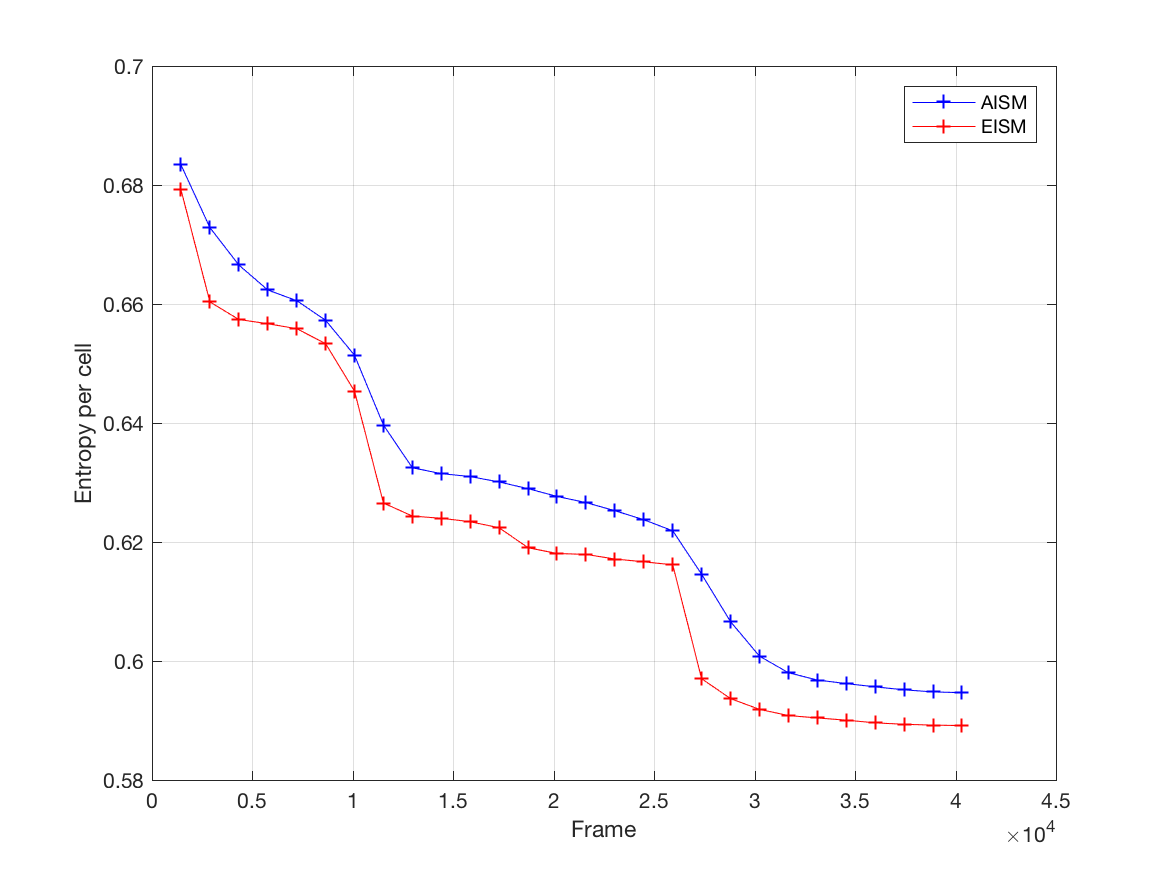
\includegraphics[width=0.7\textwidth]{entropy_frame.png}
  \caption{Entropy Histories of the Proposed Ray-By-Ray Approach and Approximate Solution}
  	\medskip
	\small
	The map entropies of the approximate inverse sensor model (blue) and the proposed exact inverse sensor model (red) show that the exact version yields a more certain occupancy grid map.
\label{fig:entropy}
\end{figure}



\paragraph{Mapping a Room with the Synergistic Approach}

Next, we compare the same approximate inverse sensor model against the synergistic exact inverse sensor model.
Here, the robot maps in a two-dimensional environment composed of ten wall edges, and the robot follows a figure-eight curve, then turns around and completes the same curve in the reverse direction. Like the prior example, the same set of measurements updated each second are used with both occupancy grid mapping algorithms to construct the map.
The resulting maps are illustrated in Figure \ref{fig:NumResOccProbs} for both algorithms, where it is shown that the proposed algorithm yields a substantially more accurate and clear map with less uncertainty. 

\begin{figure}
%    \centering{
%    \begin{subfigure}[t]{0.4\columnwidth}
%        \centering
%        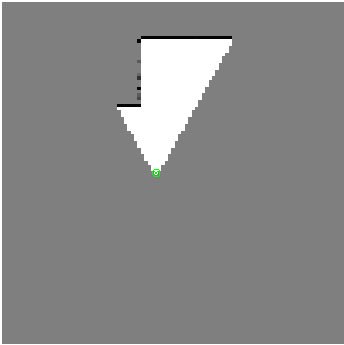
\includegraphics[width=0.7\columnwidth]{Compare_ISM_1.png}
%        \caption{Map at $t=0$ sec (exact)}
%    \end{subfigure}
%    \begin{subfigure}[t]{0.4\columnwidth}
%        \centering
%        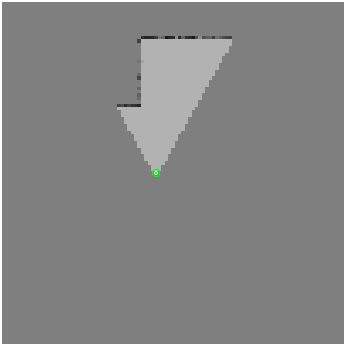
\includegraphics[width=0.7\columnwidth]{Compare_Approx_1.png}
%        \caption{Map at $t=0$ sec (approx.)}
%    \end{subfigure}
%    }
    \centering{
    \begin{subfigure}[t]{0.4\columnwidth}
        \centering
        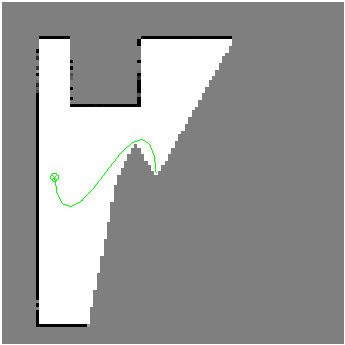
\includegraphics[width=0.7\columnwidth]{Compare_ISM_2.png}
        \caption{Map at $t=13$ sec (exact)}
    \end{subfigure}
    \hspace*{-0.05\columnwidth}
    \begin{subfigure}[t]{0.4\columnwidth}
        \centering
        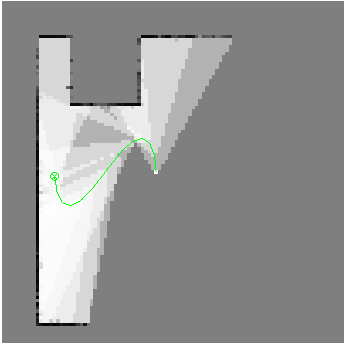
\includegraphics[width=0.7\columnwidth]{Compare_Approx_2.png}
        \caption{Map at $t=13$ sec (approx.)}
    \end{subfigure}
    }
    \centering{
    \begin{subfigure}[t]{0.4\columnwidth}
        \centering
        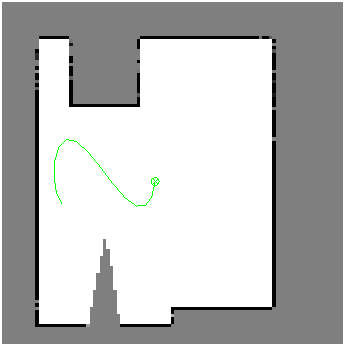
\includegraphics[width=0.7\columnwidth]{Compare_ISM_3.png}
        \caption{Map at $t=25$ sec (exact)}
    \end{subfigure}
    \hspace*{-0.05\columnwidth}
    \begin{subfigure}[t]{0.4\columnwidth}
        \centering
        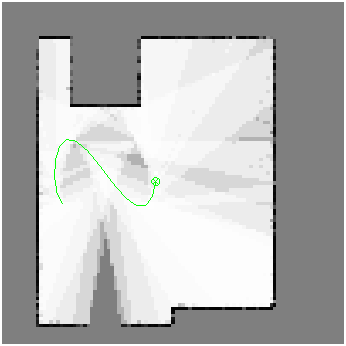
\includegraphics[width=0.7\columnwidth]{Compare_Approx_3.png}
        \caption{Map at $t=25$ sec (approx.)}
    \end{subfigure}
    }
    \centering{
    \begin{subfigure}[t]{0.4\columnwidth}
        \centering
        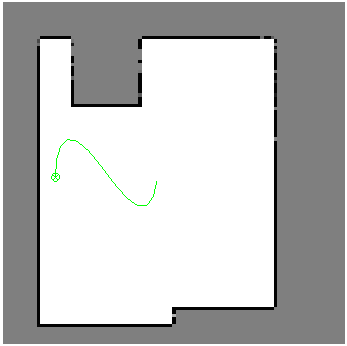
\includegraphics[width=0.7\columnwidth]{Compare_ISM_4.png}
        \caption{Map at $t=38$ sec (exact)}
    \end{subfigure}
    \hspace*{-0.05\columnwidth}
    \begin{subfigure}[t]{0.4\columnwidth}
        \centering
        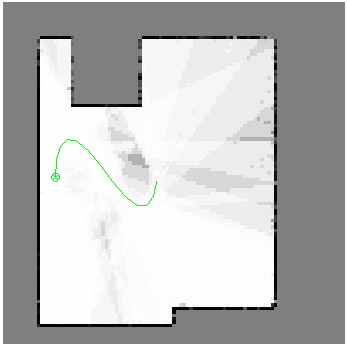
\includegraphics[width=0.7\columnwidth]{Compare_Approx_4.png}
        \caption{Map at $t=38$ sec (approx.)}
    \end{subfigure}
    }
    \centering{
    \begin{subfigure}[t]{0.4\columnwidth}
        \centering
        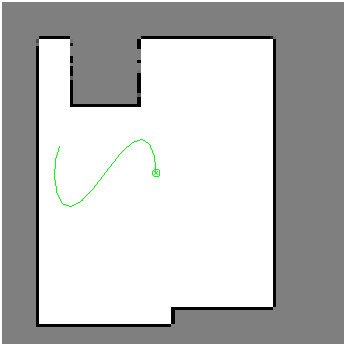
\includegraphics[width=0.7\columnwidth]{Compare_ISM_5.png}
        \caption{Map at $t=50$ sec (exact)}
    \end{subfigure}
    \hspace*{-0.05\columnwidth}
    \begin{subfigure}[t]{0.4\columnwidth}
        \centering
        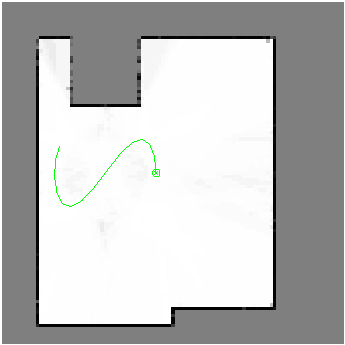
\includegraphics[width=0.7\columnwidth]{Compare_Approx_5.png}
        \caption{Map at $t=50$ sec (approx.)}
    \end{subfigure}
    }
    \caption{Comparison of Proposed Synergistic Approach with Approximate Solution}
	\medskip
	\small
	A robot (green crossed circle, green curve of its previous $13$ seconds) measures a room with a Kinect depth sensor. Grid cells are either known as free (white) or occupied (black), or uncertain (gray).
\label{fig:NumResOccProbs}
\end{figure}


The change of the map entropy over time, and the entropy of the completed maps, for both methods are depicted in Figure \ref{fig:NumResOccH}. The subfigure \ref{fig:NumResOccHa} illustrates that the proposed exact inverse sensor model exhibits rapid decreases of entropies, and smaller entropies always. The resulting terminal map obtained from the proposed approach, shown in the subfigure \ref{fig:NumResOccHb}, has less uncertainty than \ref{fig:NumResOccHc} constructed by the approximate model. In short, the proposed approach is more efficient at extracting information about the environment from the same set of set measurements. 


\begin{figure}
    \centering{
    \begin{subfigure}[t]{0.8\columnwidth}
        \centering
        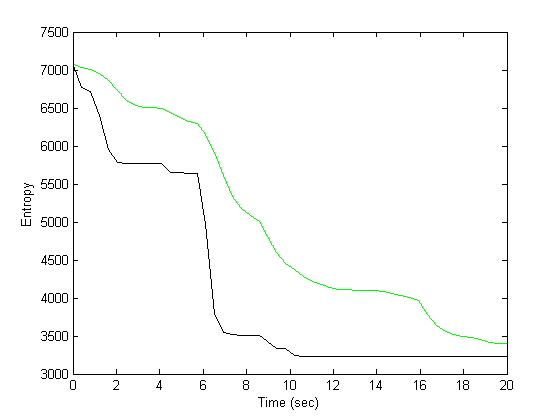
\includegraphics[width=0.7\columnwidth]{EntropyEvolution.png}
        \caption{Entropy (black: exact model, green: approx.)}
        \label{fig:NumResOccHa}
    \end{subfigure}
}
    \centering{
    \begin{subfigure}[t]{0.4\columnwidth}
        \centering
        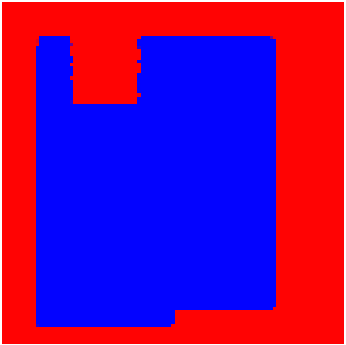
\includegraphics[width=0.7\columnwidth]{Compare_ISM_H.png}
        \caption{Entropy map at $t=50$ (exact)}
        \label{fig:NumResOccHb}
    \end{subfigure}
    \begin{subfigure}[t]{0.4\columnwidth}
        \centering
        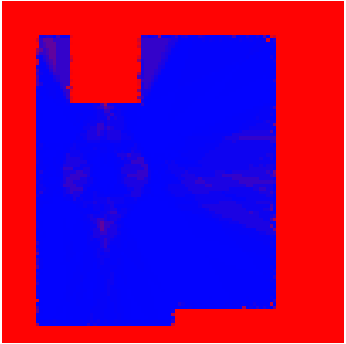
\includegraphics[width=0.7\columnwidth]{Compare_Approx_H.png}
        \caption{Entropy map at $t=50$  (approx.)}
        \label{fig:NumResOccHc}
    \end{subfigure}
    }
    \caption{Map Uncertainty Comparison Between Proposed Synergistic Approach and Approximate Solution}
	\medskip
	\small
	Entropy serves as a measure of uncertainty of the occupancy grid, where more blue regions are more certain, and red regions are more uncertain. The uncertainty is always less when the exact solution is applied.
\label{fig:NumResOccH}
\end{figure}


% I think I'll skip this trivial result:
%\subsection{Kinect Measurement Scan Analysis}
%% ACC16 Single scan exact/approx. comparison




\section{Conclusions}

In this chapter, we presented the exact solution to the inverse sensor model for a single measurement ray, then extended this result to 2D occupancy grids. Measurement scans were analyzed with two techniques, namely ray-by-ray and synergistic combinations. Then, numerical results show how both proposed solutions outperform existing approximate solutions. Upon further study, the ray-by-ray approach has proven more robust against localization errors and changing environments because the rays are not assumed completely independent. Therefore, the ray-by-ray approach is applied to the subsequent proposals, numerical simulations, and experimental results.






% !TEX root = ../thesis-sample.tex

\chapter{Autonomous Exploration in 2D Space} \label{chap:ae2D}

The goal of autonomous exploration is to select robotic actions designed to minimize map uncertainty, thereby maximizing map information gain. We formulate autonomous exploration as an optimization problem to determine a policy that accounts for map uncertainty and travel cost.

\section{Entropy-Based Exploration}

In this section, we define Shannon's entropy as a measure of map uncertainty, and present a novel approach to predict future entropy from an arbitrary ray. Then we discuss computational modifications for real-time implementation.

\subsection{Shannon's Entropy}

Here we present how the probabilistic properties of an occupancy grid map provide key information about the uncertainty of the space for motion planning. Shannon's entropy commonly serves as an uncertainty measure~\cite{StaGriBur05}. Provided grid cell probabilities of map $m$, Shannon's entropy is defined as
\begin{align}
\label{eqn:ShannonsEntropyCell}
H(P(\mathbf{m}_i))&=-P(\mathbf{m}_i)\log{P(\mathbf{m}_i})-P(\bar{\mathbf{m}}_i)\log{P(\bar{\mathbf{m}}_i}),
\\
\label{eqn:ShannonsEntropyMap}
H(P(m))&=\sum_{i=1}^{n_m}H(P(\mathbf{m}_i)),
\end{align}
for an individual cell and the entire map, respectively.
Thus, entropy is maximized when $P(\mathbf{m}_i)=0.5$, which corresponds to the largest uncertainty; similarly, entropy is minimized as $P(\mathbf{m}_i)$ approaches $0$ or $1$, which corresponds to the smallest uncertainty. %; thus Shannon's entropy is a measure of uncertainty.



\subsection{Expected Information Gain}

Suppose a future pose candidate and its associated future measurement scan is $X_c=\braces{x_c,R_c}$ and $Z_c$, respectively, where $c\in\mathcal C$ such that $\mathcal C=\braces{1,2,...,n_c}$ accounts for all $n_c$ candidates under consideration for the next robot pose. The current pose of the robot is \emph{not} $X_c$ in general, so any change to the probabilistic map from $X_c$ must be predicted. Much like the probabilistic mapping, this is achieved ray-by-ray~\cite{KauAiLee16,KauTakAiLee17}. Considering that all grid cell probabilities are conditioned on the history of poses $X_{1:t}$ and measurement scans $Z_{1:t}$, these terms are removed from the remaining equations of this dissertation for simplicity (excluding Appendices). 

\begin{prop}
\label{prop:ExpectedH}
For candidate ray $z_c$, the expected entropy is
\begin{align}
\label{eqn:DiscExpEntropyRay}
&\text{E}[H(P(m|x_c,z_{c}))]=\sum_{k=1}^{n_{r}+1}\bigg\{H(P(m|x_c,z_{c,k}))P(z_{c,k}|x_c)\bigg\},
\end{align}
where $z_{c,k}$ refers to the distance from $x_c$ to the $k$-th grid cell along the measurement ray. The first term of the summation of \refeqn{DiscExpEntropyRay}, namely $H(P(m|x_c,z_{c,k}))$, is obtained with entropy definitions \refeqn{ShannonsEntropyCell}, \refeqn{ShannonsEntropyMap} and the inverse sensor model \refeqn{RayISMAnswer}--\refeqn{Unnormalized}. The second term is derived from \refeqn{allEta} with
\begin{align}
\label{eqn:ProbMeas}
P(z_{c,k}|x_c)&=\frac{p(z_{c,k}|x_c)}{\sum_{i=1}^{n_{r}+1}p(z_{c,i}|x_c)}=\frac{\eta_{c,k}^{-1}}{\sum_{i=1}^{n_{r}+1}\eta_{c,i}^{-1}},
\end{align}
where $\eta_{c,k}$ refers to the normalizer based on the measurement $z_{c,k}$.
The expected negative entropy change for candidate pose $X_c$ is equivalently the expected information gain from ray $z_c$,
\begin{align}
\label{eqn:expectedInfoGainRay}
\mathcal I(X_c,z_c)&=H(P(m))-\text{E}\left[H(P(m|X_c,z_c))\right].
\end{align}
\end{prop}
\begin{proof}% TODO: add ref?
See Appendix B.
\end{proof}

The proposed approach discretizes the measurement according to assumptions of occupancy grid mapping, and exploits the probabilistic properties uncovered by the proposed inverse sensor model. These are used to directly calculate the expected value of map entropy for a single measurement ray. 





\subsection{Computational Limitations and Approximations}

The computational order for each measurement ray is $\mathcal O(n_{r}^2)$ since the summations of \refeqn{ProbMeas} are embedded in \refeqn{DiscExpEntropyRay}. However, several of those intersections provide negligible information since the probability of the measurement ray capturing certain cell depths is close to zero.

The approximation of expected ray entropy provides a method to reduce the computation of \refeqn{expectedInfoGainRay} substantially. This goal is achieved by systematically selecting a smaller set of grid cells to consider over the summations of \refeqn{DiscExpEntropyRay} and \refeqn{ProbMeas}.
The smaller set is determined by the probability that each cell is captured by the measurement ray, known as the detection probability. This can be found recursively as
\begin{align}
\label{eqn:ProbOfFirstCell}
P(\mathbf{r}_{k+})%\nonumber\\&
=\bigg\{\prod_{j=0}^{k-1}P(\bar{\mathbf{r}}_{j})\bigg\}P(\mathbf{r}_{k}),
\end{align}
which is the probability that $\mathbf{r}_{k}$ is the closest occupied grid cell based on past poses and measurement scans, independent of cells beyond the $k$-th cell from $x_c$.
Let $\hat n>0$ be a fixed number of grid cells such that $\hat n\leq n_{r}+1$.
Let $\hat{r}$ correspond to the grid cells that yield the $\hat{n}$ maximum values of \refeqn{ProbOfFirstCell} (the $\hat n$ most likely ray detections), indexed by increasing distance from candidate location $x_c$.
By replacing the reduced map $r$ with $\hat{r}$ and changing the summation limits to $\braces{1,2,...,\hat n}$ in \refeqn{DiscExpEntropyRay} and \refeqn{ProbMeas}, the order of computation is reduced to $\mathcal O({\hat{n}}^2)$.
Even though the value of $n_{r}$ is different among various measurement rays in general, $\hat n$ is fixed for all rays, so the computational order is fixed as well.
In short, this method reduces the required computation substantially by systematically neglecting those grid cells with little effect. It can be noted that if $\hat n=n_{r}+1$, the ray objective function is computed without approximation.


\paragraph{Algorithm} We present an algorithm pseudocode providing the necessary steps to obtain the objective function for a single measurement ray (Algorithm \ref{alg:RayExpectedEntropyGain}). Much like the algorithm pseudocode for the ray-by-ray inverse sensor model (Algorithm \ref{alg:RayByRayISM}), the variable $a_\text{temp}$ serves as an intermediate variable designed to avoid repeated calculations.
Since this algorithm operates as a function, fixed indices and condition variables are removed for simplification. 

\vspace*{0.05\columnwidth}
\begin{algorithm}[H]
	Function: $\mathcal I_\text{ray}=\text{RayExpInfoGain}(x,P(r),z_{1:n_{r}})$\;
	Initialize $P(\bar{\mathbf{r}}_{0})=P(\hat{\bar{\mathbf{r}}}_{0})=P(\bar{\mathbf{r}}_{n_{r}+1})=1$\;
	\For{$k = 1,2,\ldots,n_{r}+1$}{
		$P(\mathbf{r}_{k+}) = P(\bar{\mathbf{r}}_{0:k-1})P(\mathbf{r}_{k})$\;
		$P(\bar{\mathbf{r}}_{0:k})=P(\bar{\mathbf{r}}_{0:k-1})(1-P(\mathbf{r}_{k}))$\;
	}
	Find $\hat r\subset r$ of the $\hat n$ greatest values of 
	$\braces{P(\mathbf{r}_{1+}),P(\mathbf{r}_{2+}),\ldots,P(\mathbf{r}_{(n_{r}+1)+})}$\;
	\For{$k = 1,2,\ldots,\hat{n}$}{
		$P(\hat{\mathbf{r}}_{k+}) = P(\hat{\bar{\mathbf{r}}}_{0:k-1})P(\hat{\mathbf{r}}_{k})$\;
		$P(\hat{\bar{\mathbf{r}}}_{0:k})=P(\hat{\bar{\mathbf{r}}}_{0:k-1})P(\hat{\bar{\mathbf{r}}}_{k})$\;
	}
	\For{$k_\text{m}=1,2,\ldots,\hat n$}{
		Initialize $\eta^{-1}_{k_\text{m}}=0$\;
		\For{$k_\text{c}=1,2,\ldots,\hat n$}{
			$a_\text{temp}=P(\hat{\mathbf{r}}_{k_\text{c}+})p(z_{k_\text{m}}|\hat{\mathbf{r}}_{k_\text{c}+},x)$\;
			$\tilde P(\hat{\mathbf{r}}_{k_\text{c}}|x,z_{k_\text{m}})=P(\hat{\mathbf{r}}_{k_\text{c}})\eta^{-1}_{k_\text{m}}+a_\text{temp}$\;
			$\eta^{-1}_{k_\text{m}}=\eta^{-1}_{k_\text{m}}+a_\text{temp}$\;
		}
		$P(\hat{\mathbf{r}}_{k_\text{c}}|x,z_{k_\text{m}})=\eta_{k_\text{m}}\tilde P(\hat{\mathbf{r}}_{k_\text{c}}|x,z_{k_\text{m}})$ for all $k_\text{c}=1,2,\ldots,\hat n$\;
	}
	$P(z_{k_\text{m}}|x)=\frac{\eta^{-1}_{k_\text{m}}}{\sum_{i=1}^{\hat n}\eta^{-1}_{i}}$ for $k_\text{m}=1,2,\ldots,\hat n$\;
	Initialize $\mathcal I_\text{ray}=0$\;
	\For{$k_\text{c}=1,2,\ldots,\hat n$}{
		$\mathcal I_\text{ray}=\mathcal I_\text{ray}+H(P(\hat{\mathbf{r}}_{k_\text{c}}))$\;
		\For{$k_\text{m}=1,2,\ldots,\hat n$}{
			$\mathcal I_\text{ray} = \mathcal I_\text{ray}-H(P(\hat{\mathbf{r}}_{k_\text{c}}|x_c,z_{k_\text{m}}))P(z_{k_\text{m}}|x_{c})$\;
		}
	}
	Return: $\mathcal I_\text{ray}$\\
\caption{Expected Information Gain from a Measurement Ray}
\label{alg:RayExpectedEntropyGain}
\end{algorithm}



\paragraph{Numerical Justification for the Approximation}

The purpose of this numerical example is to provide evidence that the approximations are reasonable and increase the algorithm speed substantially.
Since a measurement ray returns a range in a single direction, we only consider a 1D map where the grid cells have spacing $\alpha=0.2$ m, and the properties of the range sensor are based on the Microsoft Kinect~\cite{PirRutBisSch11,KhoElb12} with maximum reading depth $z_\text{max}=4$ m ($20$ grid cells inside the sensor FOV). The goal is to compare the expected entropy $\text{E}[H(P(m|x_c,z_{c}))]$ from \refeqn{DiscExpEntropyRay} and with an approximation $\text{E}[H_\text{approx}(P(m|x_c,z_{c}))]$, which only considers $\hat n$ grid cells with highest detection probability \refeqn{ProbOfFirstCell}.

We consider $100$ probabilistic maps to obtain Monte Carlo results to evaluate the approximate entropy. In every Monte Carlo trial, each grid cell has an $80\%$ chance of being free and a $20\%$ chance of receiving an a priori probability uniformly distributed between $0$ and $1$. 
Several metrics serve to evaluate $\text{E}[H(P(m|x_c,z_{c}))]$ with $\text{E}[H_\text{approx}(P(m|x_c,z_{c}))]$. The median expected entropy change is $\text{E}[H(P(m|x_c,z_{c}))]-H(P(m|X_{1:t},Z_{1:t}))=-0.83792$. The error for the $100$ Monte Carlo cases is defined simply as
\begin{align}
e_{H}&=\frac1{100}\sum_{i=1}^{100}\text{abs}\bigg(\text{E}[H(P(m|x_c,z_{c}))]-\text{E}[H_\text{approx}(P(m|x_c,z_{c}))]\bigg).
\end{align}
The Monte Carlo trials are repeated for $\hat n=\braces{1,2,\ldots,10}$ and the results are plotted in Figure \ref{fig:ApproxJust}.
This example shows a typical case when the summation limits generated from \refeqn{ProbOfFirstCell} have only small effects on \refeqn{DiscExpEntropyRay}, while providing very large improvements in reducing computation.

\begin{figure}
	\centering
    	\begin{subfigure}[b]{0.45\textwidth}
        		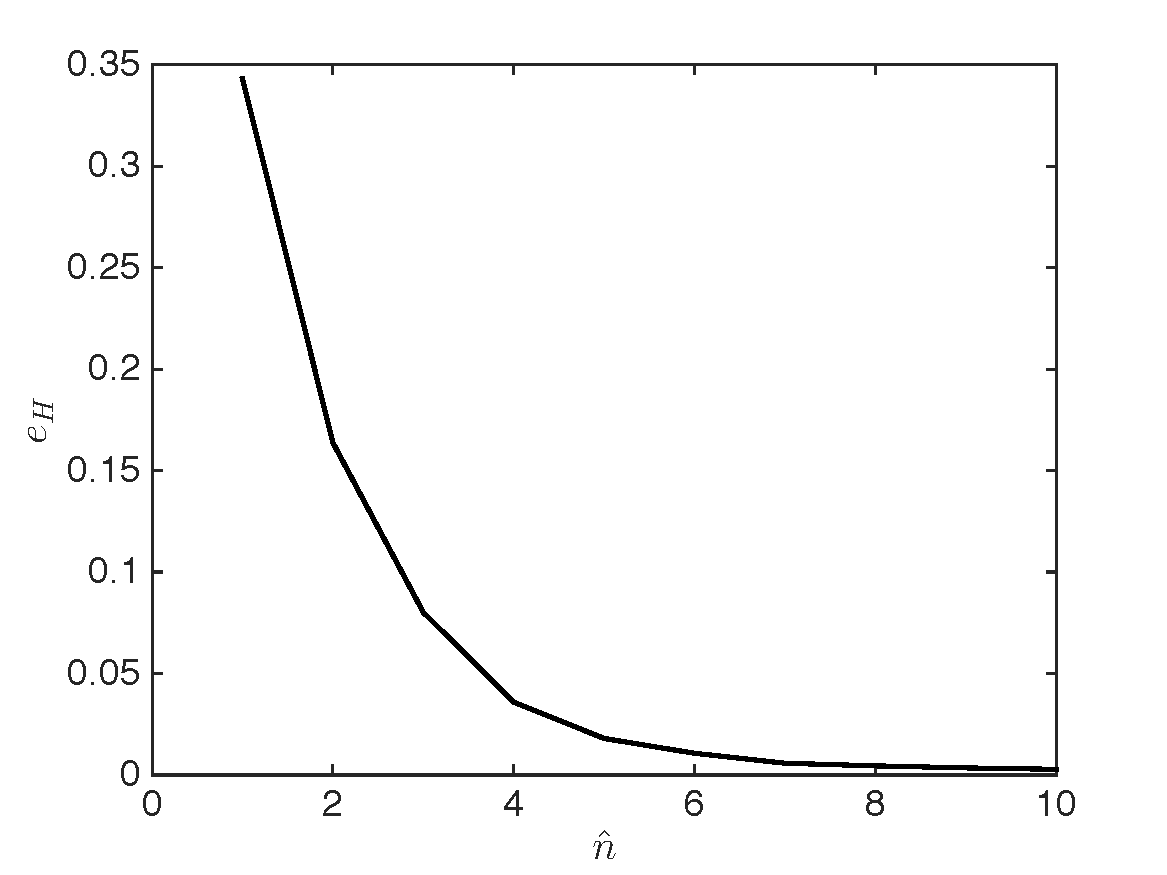
\includegraphics[width=\textwidth]{JustifyApprox_eH.pdf}
        		\caption{Entropy Error}
        		\label{fig:H_err}
    	\end{subfigure}
	\begin{subfigure}[b]{0.45\textwidth}
        		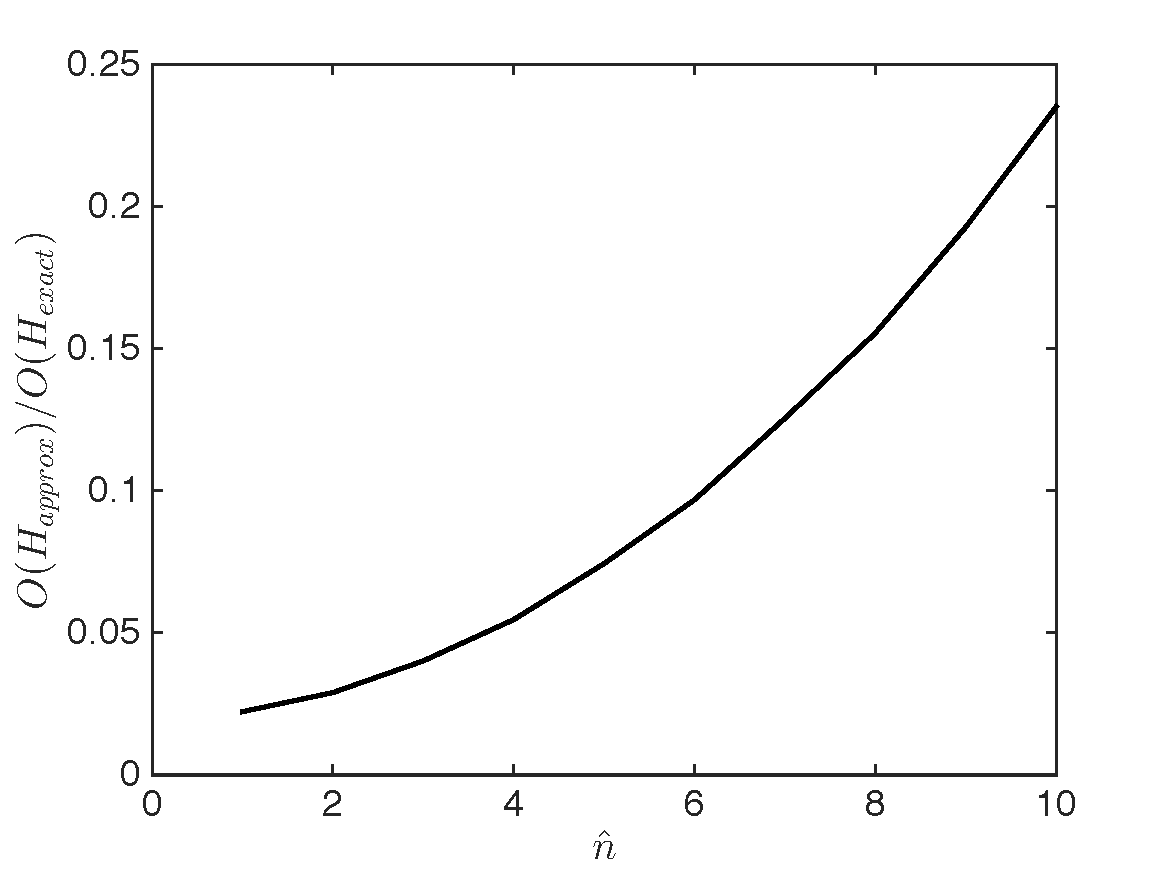
\includegraphics[width=\textwidth]{JustifyApprox_t.pdf}
        		\caption{Computation Ratio}
        		\label{fig:H_comp_ratio}
    	\end{subfigure}
\caption{The entropy error is decreased at the cost of increasing computation time in this Monte Carlo 1D measurement ray expected entropy case.}
\label{fig:ApproxJust}
\end{figure}





\section{Future Pose Optimization}

In this section, we show how expected entropy changes from single measurement rays can be integrated into predicting the expected information gain of measurement scans. This metric, and a cost associated with travel time, are combined to determine an optimal future pose and collision-free path in a 2D environment.

\subsection{Optimal Pose from Sample Rays}
\label{sec:OptimalPose2DMap}

The objective is to choose a future pose that minimizes the map uncertainty, such that the robot can autonomously move toward this optimal goal. The robot pose is selected among various positions and attitudes. Since searching over all locations and attitudes would require infinite computational resources, these search spaces are discretized into a limited number of robot attitudes and positions.
The procedure involves three steps. First, the attitude that maximizes the information gain objective function is selected at each candidate future pose location. Second, the location with the maximum objective function of all candidates is selected. Thus, the optimal attitude and the optimal location compose the optimal future pose. Finally, the robot determines and follows a collision-free path to the optimal future pose. This process is repeated, resulting in autonomous exploration.

\paragraph{Attitude Optimization}
Consider a collision-free pose candidate at an arbitrary location $x_c$. At this pose, consider $n_d$ evenly-spaced measurement rays oriented radially outward from the robot in a circular pattern (see red lines in Figure \ref{fig:OptProcess}). These rays are denoted $\braces{z_{c,1},z_{c,2},\ldots,z_{c,n_d}}$. Attitudes correspond to the rays such that the robot sensor is aligned with the ray direction, and these are denoted $\braces{R_{c,1},R_{c,2},\ldots,R_{c,n_d}}$, where the scan with attitude $R_{c,d}$ might cover several ray directions depending on the sensor FOV. We choose optimal attitude $R_c^*$ as the summation of the expected entropy changes covered by the scan,
\begin{align}
\label{eqn:FindRc}
&R_c^*=\argmax_{R_{c,d}}\sum_{z_{c,i}\in R_{c,d}\text{ FOV}}\bigg(H(P(m))
-\text{E}[H(P(m|x_c,z_{c,i}))]\bigg).
%\mathcal I_\text{ray}(x_c,z_{c,i})\right).
\end{align}

This method provides the attitude that maximizes the information gain at an arbitrary location in 2D space. The set of candidate positions that warrant consideration is determined with one of two methods, namely \emph{expanding ring} and \emph{complete Cartesian}, described next.

\paragraph{Expanding Ring}
The expanding ring technique is advantageous for searching local solutions quickly, only considering distant future poses when necessary. The key idea is that future candidate locations lie on a circular ``ring'' centered around the robot, evenly spaced around the ring (see red circles in Figure \ref{fig:OptProcess}), and the ring is expanded if certain criteria are not met. More explicitly, consider $n_c$ candidate locations denoted by $x_c\in\braces{x_1,x_2,\ldots,x_{n_c}}$ located with the distance $\delta$ away from the robot. All candidates must satisfy the inequality constraint,
\begin{align}
\label{eqn:CollisionInequalityConstraint}
P_\text{collision}(X)=1-\prod_{i\in\mathcal C_X}(P(\bar{\mathbf{m}}_i)\leq\beta,
\end{align}
where $\mathcal C_X$ is the set of grid cells falling inside a volume of preselected size around $X$ that may cause collision and $\beta>0$ is a small acceptable probability of collision. Any location that violates an inequality constraint \refeqn{CollisionInequalityConstraint} is excluded to avoid collisions. The set of optimal attitudes at each candidate location is $\braces{R^*_{1},R^*_{2},\ldots,R^*_{n_c}}$, obtained from \refeqn{FindRc}. The information gain objective function for a scan $Z_c$ captured from pose $X_c$ is
\begin{align}
\label{eqn:ObjFun}
\mathcal I(X_c)=H(P(m))-\text{E}\left[H(P(m|X_c,Z_c))\right],
\end{align}
is computed by a summation about the $n_d$ rays as %\refeqn{Objective},
\begin{align}
\label{eqn:ObjFunApprox}
\mathcal I(x_c,R_c^*)&\approx \sum_{z_{c,i}\in R_{c}^*\text{ FOV}}\bigg(H(P(m))-\text{E}\left[H(P(m|x_c,z_{c,i}))\right]\bigg),
\\
x_c^*&=\argmax_{x_c}\mathcal I(x_c,R_c^*).
\end{align}
At the optimal pose $X^*_c=(x^*_c,R^*_c)$, the resulting information gain must satisfy $\mathcal I(X_c^*)\geq\mathcal I_\text{min}$, where $\mathcal I_\text{min}$ is a minimum threshold for expected information gain; robot motion is only justified when the expected information gain is significantly large. If the minimum threshold is not met, the ring of candidate pose locations is increased such that $n_c$ and $\delta$ are multiplied by a scale function $\lambda>1$.
This process is repeated until the expected information gain of the optimal pose is at least $\mathcal I_\text{min}$, or all candidates lie in collision zones or outside map limits. %A pseudocode of the process is found in Table \ref{tab:Alg_AutomousExploration}.

The primary advantage of the expanding ring approach to search the 2D space is that the number of pose candidates need not be proportional to the map area, and that local maxima tend to fall within short distances of the current robot pose. Additionally, the distance to these poses need not be explicitly considered in the pose determination optimization because the distance costs are identical to each candidate, assuming objects do not occlude the trajectories. The main drawback is that poses outside a small local region of the robot are frequently neglected, causing the robot to repeatedly execute short motions, often without large information gains.

\paragraph{Complete Cartesian}
The complete Cartesian method to search the 2D space provides candidates located fixed distance $d$ apart in each Cartesian direction. This approach is advantageous for capturing expected information gains in regions outside of the immediate vicinity of the robot, but must be applied carefully to avoid issues with computational bottlenecks due to the potentially-large search space.

Similar to the expanding ring approach, $n_c$ candidate pose locations are considered, where those violating \refeqn{CollisionInequalityConstraint} are neglected from further consideration. However, unlike the ring expanding approach, the candidates have different distances from the robot in general, so the objective function is modified to enforce a cost on the squared distance from the current pose location $x_t$ to the candidate location $x_c$, i.e.,
\begin{align}
\label{eqn:ObjFunApproxCompleteCartesian}
\mathcal I(x_c,R_c^*,x_t)\approx \sum_{z_{c,i}\in R_{c}^*\text{ FOV}}\bigg(H(P(m))-\text{E}\left[H(P(m|x_c,z_{c,i}))\right]\bigg)-k_\text{dist}\norm{x_t-x_c}^2,
\end{align}
where weighting function $k_\text{dist}$ represents the sensitivity to avoiding large motions across the map. Furthermore, the same candidate locations are considered throughout the repeated processes of exploration, and the map cell occupancies are assumed static. Therefore, if candidate location $x_c$ fails to satisfy $\mathcal I(x_c,R_c^*,x_t)+k_\text{dist}\norm{x_t-x_c}^2\geq\mathcal I_\text{min}$, then $x_c$ need \emph{never} be considered again. Avoiding these unnecessary calculations yields a greatly lowered computational burden, particularly late in exploration where several regions are collision-free but disadvantageous to revisit.


\begin{figure}
\vspace*{0.1\columnwidth}
\centerline{
	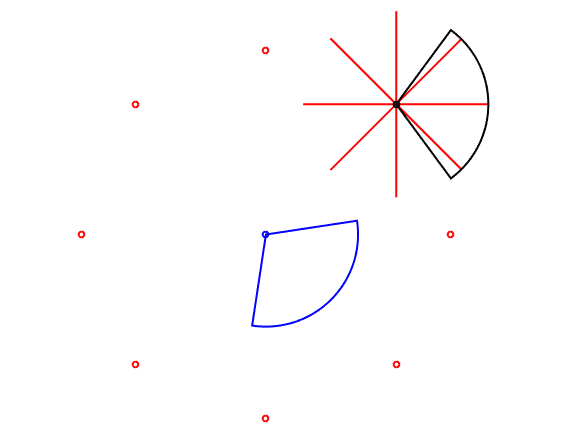
\includegraphics[height=0.35\columnwidth]{ExampleOptimalPose.png}
}
\begin{picture}(0,0)(0,0)
\setlength{\unitlength}{0.1\columnwidth}\scriptsize
\put(4.4,2.1){\color{blue}$X_t$}
\put(5.9,1.9){\color{red}$x_1$}
\put(2.9,2.0){\color{red}$x_5$}
\put(4.4,3.6){\color{red}$x_3$}
\put(4.4,0.6){\color{red}$x_7$}
\put(5.4,3.0){\color{red}$x_2$}
\put(3.3,3.1){\color{red}$x_4$}
\put(3.3,1.0){\color{red}$x_6$}
\put(5.4,1.0){\color{red}$x_8$}
\put(6.8,3.1){\color{red}$z_{2,1}$}
\put(4.5,3.1){\color{red}$z_{2,5}$}
\put(5.6,4.1){\color{red}$z_{2,3}$}
\put(5.6,2.2){\color{red}$z_{2,7}$}
\put(6.5,3.7){\color{red}$z_{2,2}$}
\put(4.9,3.8){\color{red}$z_{2,4}$}
\put(5.0,2.5){\color{red}$z_{2,6}$}
\put(6.5,2.5){\color{red}$z_{2,8}$}
\put(6.1,2.9){$X_c^*$}
\end{picture}
\caption{This figure illustrates the expanding ring method. Initially, a robot (blue circle) views down and left (blue sector). Then, the robot considers $n_c=8$ poses (red circles) as possible candidates for where to move next. For each candidate, $n_d=8$ directions are considered (red lines, only displayed on candidate location $c=2$). Then, the expected entropy of each ray is calculated. The scan (red sector) covering those rays with the largest expected entropy decrease is chosen for each candidate, and the best candidate $X_c^*$ (black circle: location, black sector: scan) is chosen to maximize information gain. Finally, Dijkstra's algorithm provides the collision-free motion between $X_t$ and $X_c^*$, and the process is repeated.
}
\label{fig:OptProcess}
\end{figure}

% TODO: move these to 3D/multi-vehicle sections
%\subsection{Travel Cost with Obstacles}
% Dijkstra's cost map
%\subsection{Optimal Pose Selection}
% Single-Vehicle argmax

\subsection{Collision-Free Motion Planning}
% Dijkstra's algorithm (after cost map), no least squares yet

There are two important steps to moving a robot on a collision-free trajectory to its optimal pose. First, Dijkstra's algorithm provides the cost map and optimal collision-free waypoints. Then, a constrained polynomial least squares trajectory serves as the desired path, which is followed by a controller.

\paragraph{Dijkstra's Search}

Dijkstra's search is naturally applied to this problem because the occupancy grid map serves nicely as a graph, and Dijkstra's algorithm provides an optimal collision-free trajectory along that graph. There are two steps to Dijkstra's algorithm: first, generate a cost map from the robot location to each grid cell on the 2D occupancy grid map. Only cells that satisfy \refeqn{CollisionInequalityConstraint} are considered to avoid possible collisions. Traveling to a neighboring cells that shares an edge costs the edge length distance $\alpha$, and the cost to travel to cells that share a corner is $\sqrt{2}\alpha$. This provides the collision-free distances to all reachable locations on the map. Second, the waypoints from a candidate pose to the current robot pose are easily obtained along the cost map using steepest descent. 


\paragraph{Constrained Polynomial Least Squares Trajectory} The trajectory to follow the path outlined by Dijkstra's algorithm is determined with a linear constrained least squares optimization, assuming the robot follows a polynomial trajectory with fixed speed. The starting and ending positions and attitudes may be constrained, and polynomials patched together for long trajectories share a common position and velocity with respect to time. Then, a controller on the robot tracks this trajectory until the robot falls within acceptable thresholds of the final optimal pose. Any control scheme for the motion of the robot can be integrated with the proposed exploration algorithm. Once the robot completes this motion, the entire process is repeated. 

\section{Numerical Examples}

Here we present two numerical examples. The first uses the expanding-ring technique in a small environment and the second considers a larger benchmark environment, so the complete Cartesian method is applied, as described in Section \ref{sec:OptimalPose2DMap}.

\subsection{Exploring a Simple Environment}
% SIMPAR numerical example (2 rooms, 1 hallway)

Here, a robot autonomously maps and explores a 2D environment composed of two rooms and one hallway. The robot models its surroundings with an occupancy grid of $15,000$ cells where grid cell edges have length $\alpha=0.2$m, composing a map with dimensions $30\text{m}\times20\text{m}$. The initial probability $P(\mathbf{m}_i)=1\times10^{-10}\approx0$ (minimum value for free space) for grid cells covered by the circular robot of radius $0.1$m and $P(\mathbf{m}_i)=0.5$ for all other cells.
At each time step, the robot receives a measurement scan, where the probabilistic properties of the sensor are taken from~\cite{PirRutBisSch11,KhoElb12}. Then, the $n_c=8$ evenly-spaced candidate locations about a circle of radius $\delta=0.5$m around the current pose location are considered, where $n_d=32$ measurement rays are evenly-spaced about the candidate location.  When no current candidates yield expected information gains above $\mathcal I_\text{min}=2$, $\lambda=1.25$ is multiplied to $n_c$ and $\delta$. The motion of the robot is restricted to movement along cells satisfying \refeqn{CollisionInequalityConstraint} with $\beta=0.01$. Dijkstra's algorithm provides collision-free motion planning.
The results are illustrated in Figure \ref{fig:AutonomousExploration}.


\begin{figure}
\centering{
    	\begin{subfigure}[b]{0.3\textwidth}
        		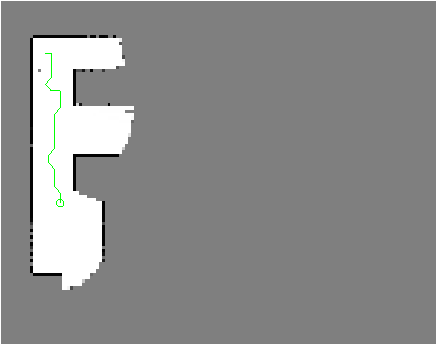
\includegraphics[width=\textwidth]{CDC16_t50.png}
        		\caption{Map at $t=50$ sec}
%        		\label{fig:}
    	\end{subfigure}
	\hspace*{0.01\columnwidth}
	\begin{subfigure}[b]{0.3\textwidth}
        		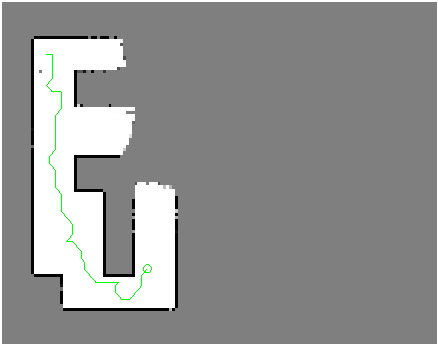
\includegraphics[width=\textwidth]{CDC16_t100.png}
        		\caption{Map at $t=100$ sec}
%        		\label{fig:}
    	\end{subfigure}
	\hspace*{0.01\columnwidth}
	\begin{subfigure}[b]{0.3\textwidth}
        		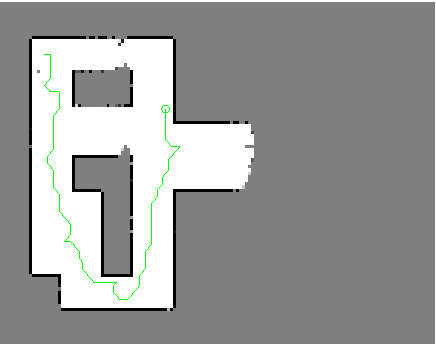
\includegraphics[width=\textwidth]{CDC16_t150.png}
        		\caption{Map at $t=150$ sec}
%        		\label{fig:}
    	\end{subfigure}
}
\centering{
    	\begin{subfigure}[b]{0.3\textwidth}
        		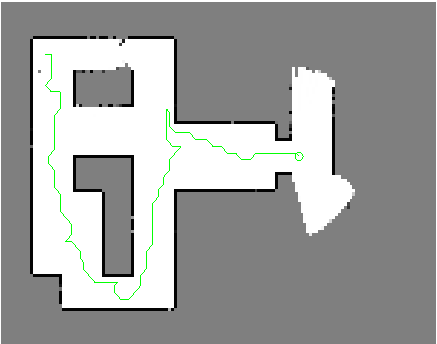
\includegraphics[width=\textwidth]{CDC16_t200.png}
        		\caption{Map at $t=100$ sec}
%        		\label{fig:}
    	\end{subfigure}
	\hspace*{0.01\columnwidth}
	\begin{subfigure}[b]{0.3\textwidth}
        		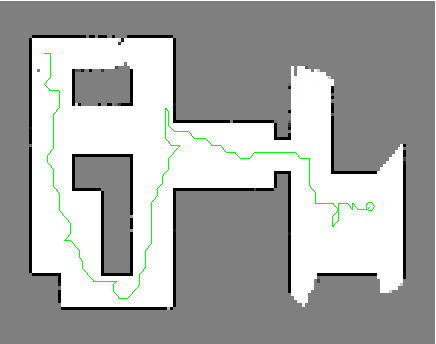
\includegraphics[width=\textwidth]{CDC16_t250.png}
        		\caption{Map at $t=250$ sec}
%        		\label{fig:}
    	\end{subfigure}
	\hspace*{0.01\columnwidth}
	\begin{subfigure}[b]{0.3\textwidth}
        		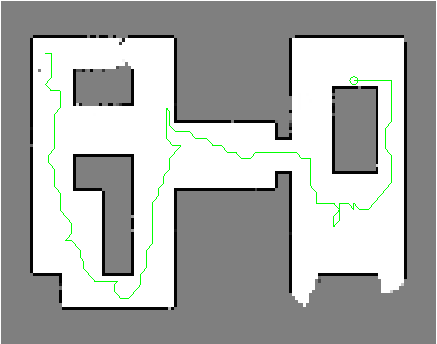
\includegraphics[width=\textwidth]{CDC16_t300.png}
        		\caption{Map at $t=300$ sec}
%        		\label{fig:}
    	\end{subfigure}
}
\centering{
    	\begin{subfigure}[b]{0.3\textwidth}
        		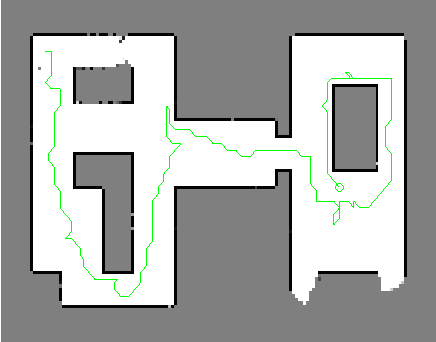
\includegraphics[width=\textwidth]{CDC16_t350.png}
        		\caption{Map at $t=350$ sec}
%        		\label{fig:}
    	\end{subfigure}
	\hspace*{0.01\columnwidth}
	\begin{subfigure}[b]{0.3\textwidth}
        		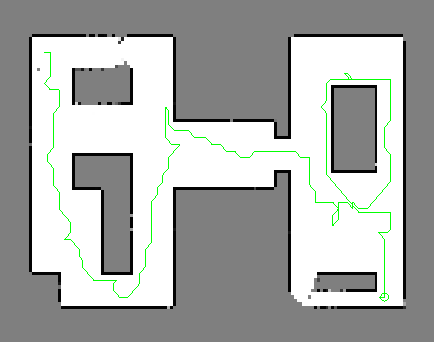
\includegraphics[width=\textwidth]{CDC16_t400.png}
        		\caption{Map at $t=400$ sec}
%        		\label{fig:}
    	\end{subfigure}
	\hspace*{0.01\columnwidth}
	\begin{subfigure}[b]{0.3\textwidth}
        		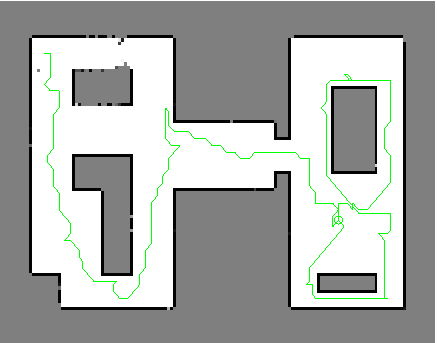
\includegraphics[width=\textwidth]{CDC16_t450.png}
        		\caption{Map at $t=450$ sec}
%        		\label{fig:}
    	\end{subfigure}
}
\caption{A robot (green circle, green marker of previous path) measures a room with a Kinect depth sensor to maximize map information gain.}
\label{fig:AutonomousExploration}
\end{figure}

Knowing only that the robot is inside free space at the beginning, the robot carefully navigates the environment while avoiding collisions. The robot motion is governed by a policy that maximizes the map information gain within its set of pose candidates, where the $\hat n=6$ is chosen to approximate the expected entropy of each ray. 
When running the exploration algorithm within the framework of the Robot Operating System (ROS), the mean computation time is $0.0194$ seconds to determine the optimal future pose and complete Dijkstra's algorithm on the occupancy grid.
The computation times for this map reached roughly $1$ second at maximum, corresponding to rare cases when the robot is locally surrounded by a highly-certain environment; this task requires evaluating many more pose candidates and motion planning over a larger terrain.

Throughout the numerical example, the robot chooses numerous actions, based directly on their expected information gains, not frontiers or predicted measurement scans. If the obstacles were known a priori, the motion planning problem would yield a simpler path; however, the autonomous exploration is based on only the information of the map that the robot generates, so the motion planning must be reevaluated repeatedly. Even with these limitations, the robot explores the vast majority of reachable space in the $450$ second period. 





\subsection{Exploring a Complicated Benchmark Environment}

Next, the proposed autonomous exploration approach is applied to the floor plan of the Intel Research Lab, illustrated in Figure~\ref{fig:intel}.
The robot explores its surroundings with an occupancy grid with $90,000$ cells where grid cell edges are $\alpha=0.1$m, composing a map with dimensions $30\text{m}\times30\text{m}$.
Similar to the prior example, the initial probability $P(\mathbf{m}_i)=1\times10^{-10}\approx0$ (minimum value for free space) is chosen for grid cells covered by the circular robot of radius of $0.3$m and $P(\mathbf{m}_i)=0.5$ for all other cells.
For added safety, cells falling within $0.6$m of the robot are considered inside the possible collision zone $\mathcal{C}_X$, from \refeqn{CollisionInequalityConstraint}, where $\beta=0.1$ is selected. 

The robot follows the complete Cartesian candidate search method to determine future poses, with $k_\text{dist}=5$ to avoid large motions with little added expected information gains. Due to the large size of the map, candidates below the expected information gain of $1.25$ are neglected from future consideration.

The time sequence of the exploration for every 5~minutes are simulated in the ROS Stage 2D environment. The corresponding simulation results are illustrated in Figure \ref{fig:IRL} and a video is available at \href{https://www.youtube.com/watch?v=5VdzKHreB_s}{\WriteBlue{https://www.youtube.com/watch?v=5VdzKHreB\_s}}.
Lighter red dots and darker blue dots in the explored area correlate to the level of information gain at those positions with low and high value, respectively. It is shown that the proposed autonomous exploration algorithm successfully mapped the complicated environment composed of a number of rooms, narrow hallways, and open spaces that are irregularly shaped.


\begin{figure}
    \centering
    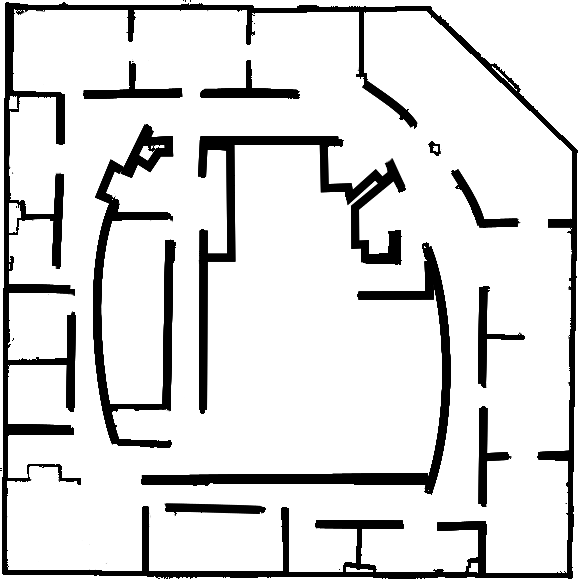
\includegraphics[width=0.4\textwidth]{intel_clean.png}
    \caption{Intel Research Lab floor plan benchmark~\cite{kummerle2009measuring}.}
\label{fig:intel}
\end{figure}


\begin{figure}[!ht]
    \centering
    \begin{subfigure}[t]{0.3\columnwidth}
        \centering
        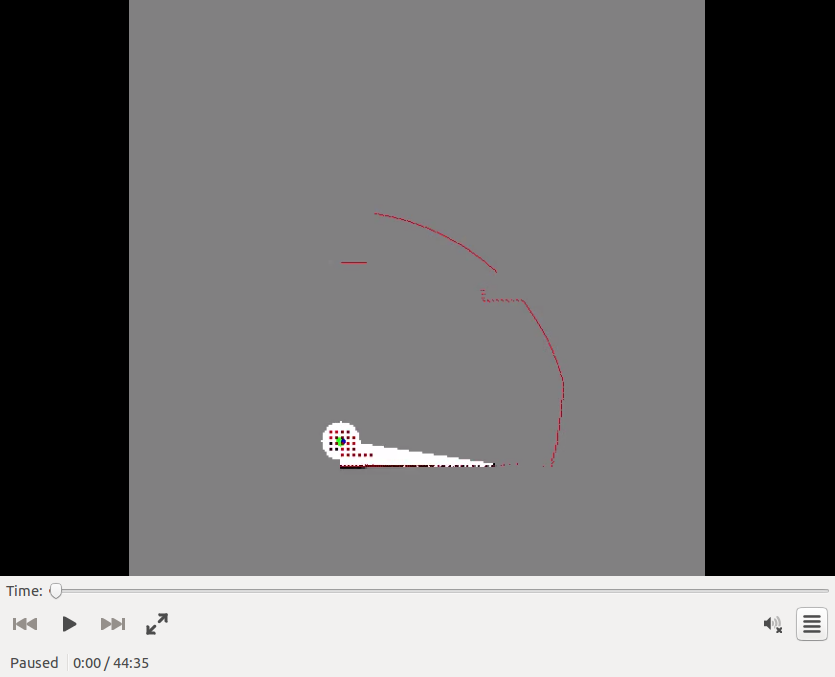
\includegraphics[trim = {4.6cm 3.8cm 4.6cm 0}, clip, width=\textwidth]{0min.png}
        \caption{$t=0$ min}
        \label{fig:IRL0min}
    \end{subfigure}
    \begin{subfigure}[t]{0.3\columnwidth}
        \centering
        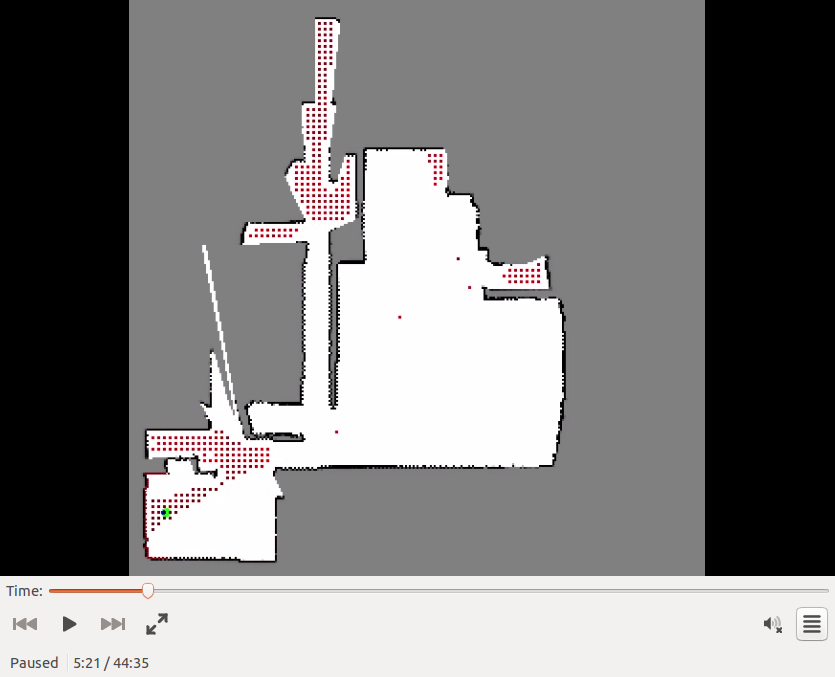
\includegraphics[trim = {4.6cm 3.8cm 4.6cm 0}, clip, width=\textwidth]{5min.png}
        \caption{$t=5$ min}
        \label{fig:IRL5min}
    \end{subfigure}
    \begin{subfigure}[t]{0.3\columnwidth}
           \centering
           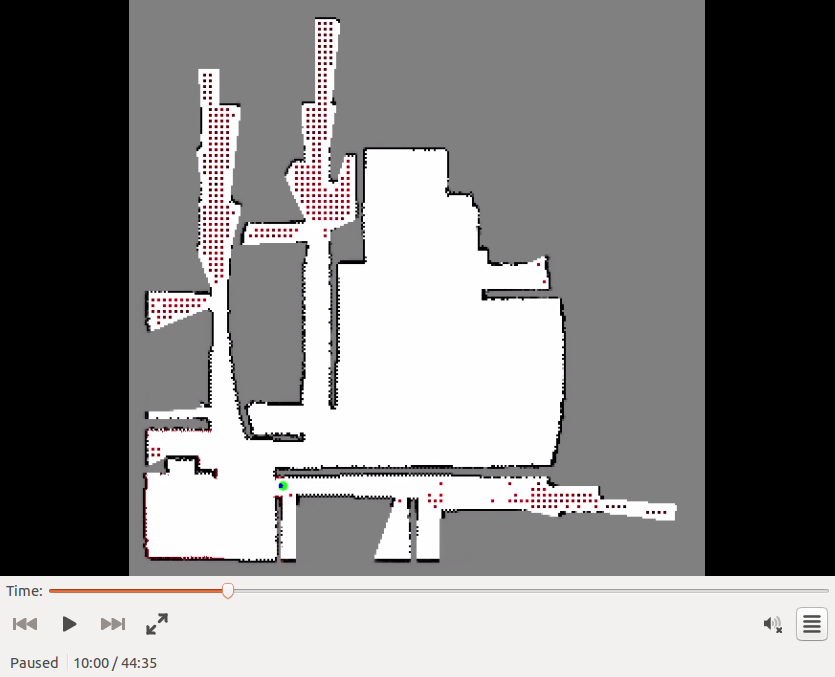
\includegraphics[trim = {4.6cm 3.8cm 4.6cm 0}, clip, width=\textwidth]{10min.png}
        \caption{$t=10$ min}
        \label{fig:IRL10min}
    \end{subfigure}
    \begin{subfigure}[t]{0.3\columnwidth}
           \centering
           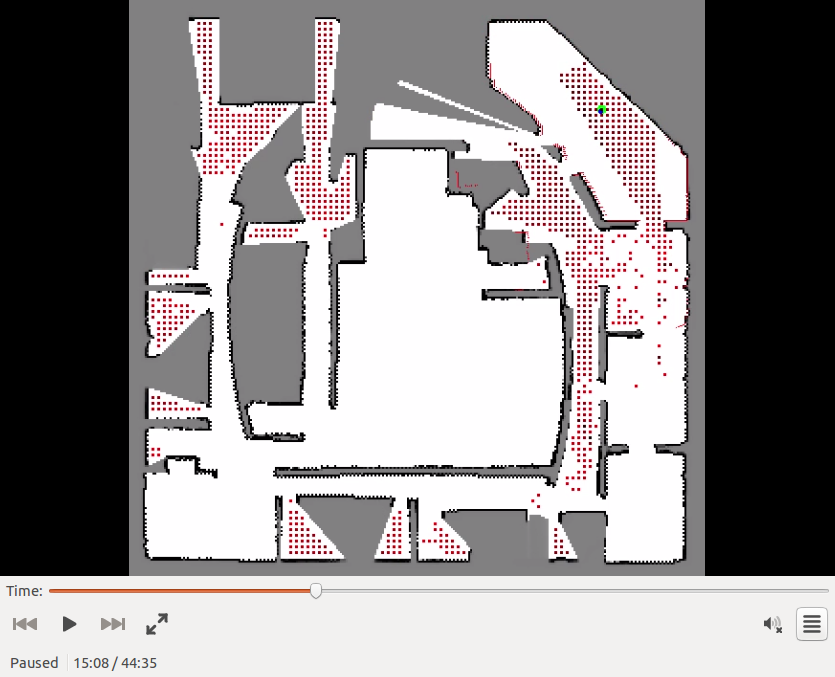
\includegraphics[trim = {4.6cm 3.8cm 4.6cm 0}, clip, width=\textwidth]{15min.png}
        \caption{$t=15$ min}
        \label{fig:IRL15min}
    \end{subfigure}
    \begin{subfigure}[t]{0.3\columnwidth}
         \centering
         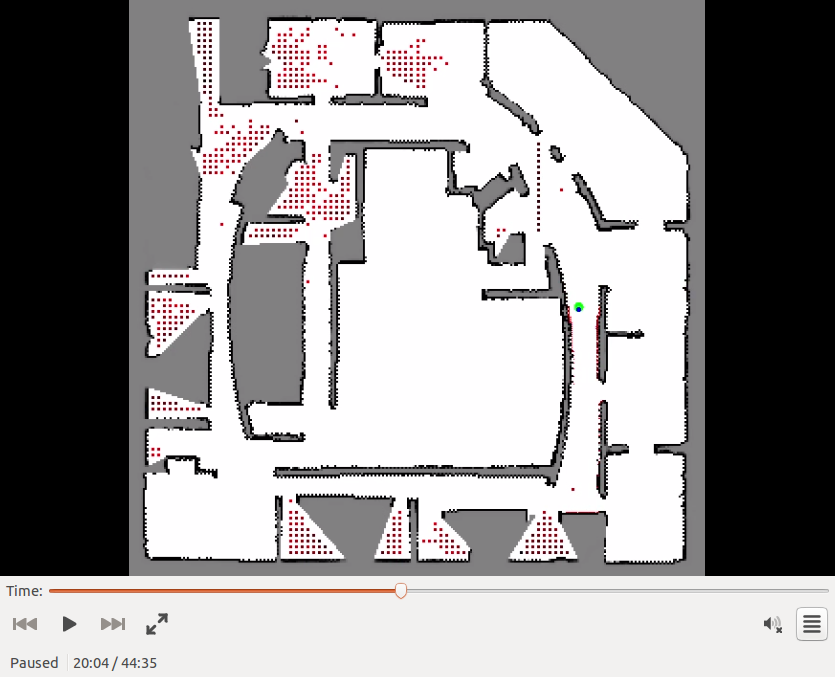
\includegraphics[trim = {4.6cm 3.8cm 4.6cm 0}, clip, width=\textwidth]{20min.png}
        \caption{$t=20$ min}
        \label{fig:IRL20min}
    \end{subfigure}
    \begin{subfigure}[t]{0.3\columnwidth}
           \centering
           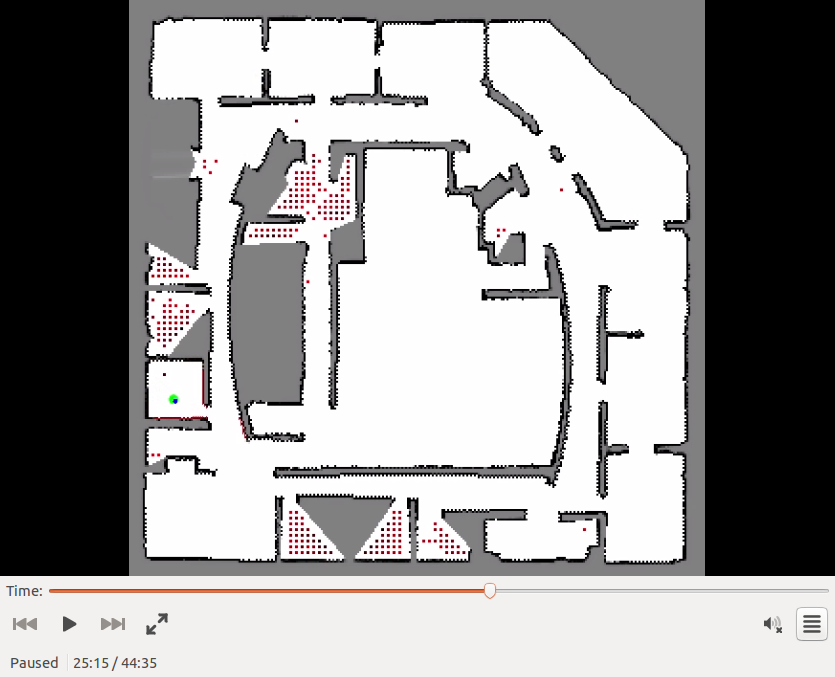
\includegraphics[trim = {4.6cm 3.8cm 4.6cm 0}, clip, width=\textwidth]{25min.png}
        \caption{$t=25$ min}
        \label{fig:IRL25min}
    \end{subfigure}
    \begin{subfigure}[t]{0.3\columnwidth}
           \centering
           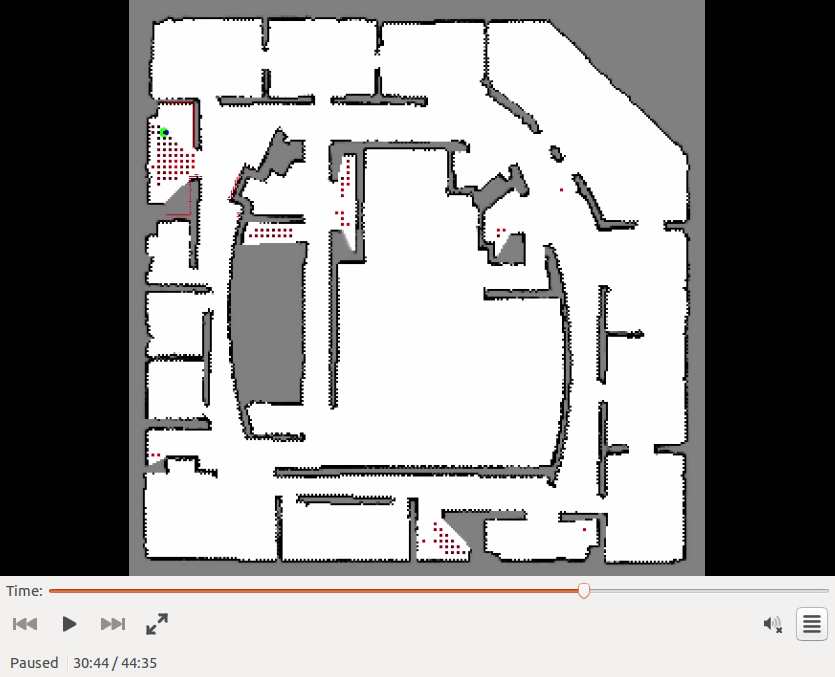
\includegraphics[trim = {4.6cm 3.8cm 4.6cm 0}, clip, width=\textwidth]{30min.png}
        \caption{$t=30$ min}
        \label{fig:IRL30min}
    \end{subfigure}
    \begin{subfigure}[t]{0.3\columnwidth}
           \centering
           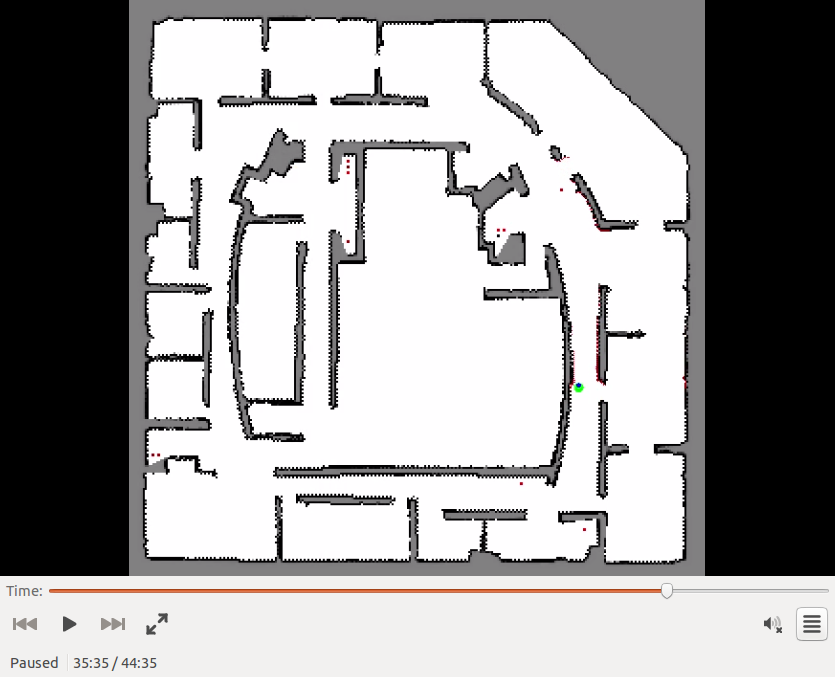
\includegraphics[trim = {4.6cm 3.8cm 4.6cm 0}, clip, width=\textwidth]{35min.png}
        \caption{$t=35$ min}
        \label{fig:IRL35min}
    \end{subfigure}
    \begin{subfigure}[t]{0.3\columnwidth}
           \centering
           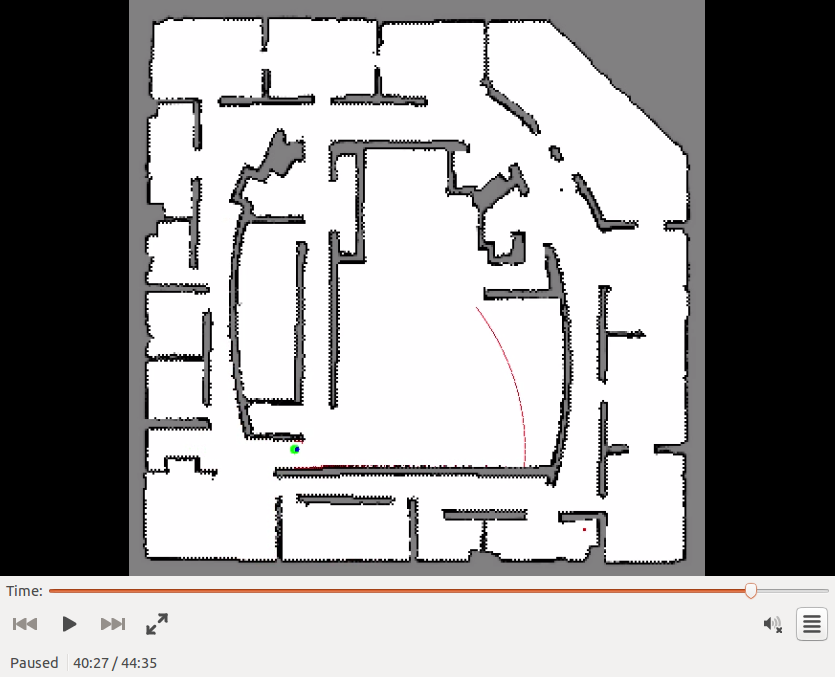
\includegraphics[trim = {4.6cm 3.8cm 4.6cm 0}, clip, width=\textwidth]{40min.png}
        \caption{$t=40$ min}
        \label{fig:IRL40min}
    \end{subfigure}
    \caption{A robot (green) measures a room in the ROS Stage simulator using the Intel Research Lab floor plan. The exact inverse sensor model is used for the autonomous exploration algorithm.}
    \label{fig:IRL}
\end{figure}



% TODO: move these to final chapter
%\section{Experimental Result}
% JINT17 9, 10, 11 (ground experiment at the NRL)

\section{Conclusions}

The proposed autonomous exploration scheme determines the expected value of entropy for various potential robotic actions. The optimal policy maximizes an objective function that includes expected information gain and travel distance. Collision-free paths to optimal poses are determined with Dijkstra's search and a constrained polynomial least squares trajectory. These are demonstrated with two numerical examples, showing the expanding ring and complete Cartesian approaches. Due to superior scalability, the complete Cartesian approach is applied to subsequent exploration algorithms in this dissertation.

% !TEX root = ../thesis-sample.tex

\chapter{Autonomous Exploration in Vertically-Uniform 3D Space} \label{chap:ae3Dsimple}

In this chapter, we introduce mapping and autonomous exploration in 3D environments. Here, we consider common spaces like rooms and hallways where objects are largely vertically-uniform. A complete 3D probabilistic map is projected onto a simpler 2D map at a fixed exploration height, where the projected map can be used for collision-avoidance and entropy predictions.

\section{Occupancy Grid Mapping in 3D}

The inverse sensor model from Chapter \ref{chap:pogm} is based on an arbitrary vector spanning 2D space. The distances from the robot to grid cells are obtained geometrically through ray casting. This method is easily extended to 3D space, and the inverse sensor model is applied identically. Since the map is updated ray-by-ray (each measurement ray is considered once by itself), this approach is extended for measurement fusion of any number of sensors; the map is updated by each ray of a scan sequentially, then the map is updated by the rays of the next scan in queue, which might have different characteristics. There are several reasons why a robot might be equipped with multiple sensors, e.g., different fields-of-view or depth sensor properties. For example, a robot may be equipped with a 2D LIDAR with highly accurate measurements, but a limited single-plane field-of-view. Then, the robot can compensate for the LIDAR limitations with an IR depth sensor that provides many more measurement rays with a 3D scan, where each ray has lower accuracy than the LIDAR rays. Since each sensor model is explicitly considered in the cell probability calculations, measurements from both sensors may serve to update the same probabilistic map. However, the impact from a LIDAR measurement with high accuracy on the probabilistic map will be greater than that of the IR depth sensor with lower accuracy. Since sensor properties are considered explicitly, the proposed 3D mapping approach can fuse the impact of measurements on the probabilistic map from different sources with different properties.

However, implementation in 3D requires several careful considerations. First, the number of cell occupancy probabilities tracked with computer memory increases by a factor of the number of cells in the added dimension. In its current form, the proposed method assumes fixed map limits, so these should be carefully selected with grid cell resolution based on available memory. Second, measurement rays spanning 3D space typically involve more intersections with grid cells. The computational orders of ray casting and the inverse sensor model are proportional to the number of grid cells along the ray $n_r$, so careful consideration must be placed on sensor limits and rays per scan that can be considered. Typically, computers small enough to be carried onboard flying robots lack the processing capabilities to update massive maps quickly, particularly because the ray-by-ray updating method requires many computations in series with large measurement scans. Therefore, an onboard computer can simply stream the sensor data, and a more powerful computer can run the mapping.

Additionally, mobile robots, particularly aerial vehicles, are frequently subject to fast movements, and the time stamps for pose estimates and depth sensor readings are not guaranteed to align. For example, the most recent pose estimate and measurement scan may have significantly different time stamps while the robot is rapidly rotating. Using these together violates the assumption that the robot pose is well-known for every measurement scan, i.e., $X_t$ and $Z_t$ are given. Therefore, pose estimates and sensor readings must be paired according to their time stamps. A useful tool that easily satisfies this goal is the Message Filters package with the Robot Operating System (ROS), where stamped poses and measurement scans are synchronized using recently-received data.

\section{Exploration in Vertically-Uniform Environments}
\label{sec:MapProjections}

Next, we describe two approaches to projecting the 3D probabilistic map onto a 2D map at the exploration height~\cite{KauTakAiLee18}. Assuming projections are sufficient is consistent with rooms and hallways with non-complex geometries.

\subsection{Collision and Entropy Maps}
Occupancy grid map cell volume is frequently smaller than the size of the robot taking measurements, particularly with highly-detailed maps. This motivates a method to simply represent locations that risk collision, referred to as a \emph{collision map} $C$. Let $k_C\geq1$ be an integer representing the minimum number of 3D grid cells that form a cube that can completely encompass the robot, i.e., the collision map cell edge length is
\begin{align}
\label{eqn:alphaC}
\alpha_C=k_C\alpha.
\end{align}
Consider the set $ m_{C,k}\subset m$ consisting of the 3D grid cells falling inside the limits of the $k$-th cell of collision map $C$, namely $\mathbf{C}_k$. Then the collision probability is
\begin{align}
P(\mathbf{C}_k)=\max{(P(\mathbf{m}_i)\ \forall \ i\in m_{C,k})}.
\end{align}
Then, the robot is only allowed to consider moving into $k$-th cell of the collision map if
\begin{align}
P(\mathbf{C}_k) \leq C_\text{thresh},
\end{align}
where $C_\text{thresh}>0$ is a maximum acceptable collision threshold, typically chosen slightly greater than $0$. In short, this conservative approach limits robotic motion to regions with a low risk of collision while neglecting objects far above or below the exploration plane.

In a similar method, \emph{entropy map} $E$ determines cells based on the entropy metric of \refeqn{ShannonsEntropyCell} over a different subset of cells. Let the $E$ be a 2D map composed of cells with edge length $\alpha$ located at the exploration height. Let the set $ m_{E,k}\subset m$ be the cells directly above and below the $k$-th cell of $E$, neglecting any 3D cells located lower than the floor height. Selecting this set is advantageous because measurements are assumed not to penetrate occupied cells (edge length $\alpha$) and measurement rays are typically not closely-aligned with the third axis of the inertial frame (vertically long set). Furthermore, any cells located below the floor, which cannot be reached, should not impact the uncertainty of the space. Then, the occupancy probability of the $k$-th entropy map cell is selected as
\begin{align}
\label{eqn:ProbEntropyMap}
P(\mathbf{E}_k)=\argmax_{P(\mathbf{m}_i)}(H(P(\mathbf{m}_i))\ \forall \ i\in m_{E,k}).
\end{align}
After several measurements of the cells belonging to $ m_{E,k}$, it is common for $H(P(\mathbf{E}_k))\approx0$, which implies that these cells are well-known. However, this does not imply that the captured space is \emph{entirely} free or occupied (e.g. an object on the ground that does not breach the upper map boundary), so applying \refeqn{ProbEntropyMap} alone could arbitrarily set $P(\mathbf{E}_k)$ close to $0$ or $1$. This can have damaging effects on the expected information of cells beyond the $k$-th cell. Let $P_\text{min}>0$ be a lower bound such that $H(P_\text{min})=H(1-P_\text{min})\approx0$. If $H(P(\mathbf{E}_k))\leq H(P_\text{min})$, then this probability is corrected to
\begin{align}
P(\mathbf{E}_k)= 
\begin{cases}
    P_\text{min},			& \text{if } \text{mean}(P(\mathbf{m}_i)\ \forall \ i\in m_{E,k})\leq0.5\\
    1-P_\text{min},              & \text{otherwise}
\end{cases},
\end{align}
where the first case corresponds to mostly open space and the second case corresponds to mostly occupied space (e.g. walls and objects). In short, the candidates are only considered if they can be reached over collision map $C$ via Dijkstra's search, and the information gains of the reachable candidates are predicted using entropy map $E$.

\subsection{Collision and Entropy Combination Map}
The second proposed technique combines the advantages of both the collision and entropy maps into a 2D projected occupancy grid map, which can be used for both tasks. Let the \emph{collision and entropy combination map} $ m_\text{2D}$ be a 2D projected map located at the exploration height with grid cell edges the same as the collision map, namely $\alpha_C$ from \refeqn{alphaC}, using the same subset of grid cells from the collision map, namely $ m_C$. Considering that the cells begin with uniform probability $P_\text{init}$ where $0<P_\text{init}<1$, define a threshold $P_\text{thresh}$ such that $P_\text{init}<P_\text{thresh}<1$. Then, the probability assigned to the $k$-th grid cell of $ m_\text{2D}$, namely $\mathbf{m}_{\text{2D},k}$ is
\begin{align}
\label{eqn:CombinationProjection2DMap}
P(\mathbf{m}_{\text{2D},k})= 
\begin{cases}
    P(\mathbf{C}_k),			& \text{if }P(\mathbf{C}_k)\geq P_\text{thresh}\\
    \min{(P(\mathbf{m}_i)\ \forall \ i\in m_{C,k})},              & \text{otherwise}
\end{cases}.
\end{align}

This approach has several advantages. First, measurements must enter the vicinity of the $k$-th cell for $P(\mathbf{m}_{\text{2D},k})$ to change from $P_\text{init}$. Without prior measurements, capturing $P(\mathbf{m}_{\text{2D},k})$ produces a large reward for the expected information gain in \refeqn{ObjFun}. Second, the value of $P_\text{thresh}$ can be modified based on how conservative the collision risk assessment for a robot should be. Additionally, when $P(\mathbf{m}_{\text{2D},k})<P_\text{thresh}$, this event tends to favor free cells such that expected information gains of cells beyond the $k$-th cell have greater impact on exploration. Furthermore, a single map is simpler, and since cell sizes satisfy $\alpha_C\geq\alpha$, it follows that $n_r$ can only be decreased with $\alpha_C$, thereby increasing computational speed.

\section{Numerical Example}
\label{sec:Compare2MapProjections}

The following numerical example involves a simulated quadrotor taking measurements of a large room and generating a 3D occupancy grid map. Separate collision and entropy map projections are used for autonomous exploration.

\subsection{Software Structure}
%        A.      Software Structures
%                list and explain ROS nodes

The Robot Operating System (ROS) provides an excellent framework for several programs, referred to as \emph{nodes}, to communicate easily. These are mostly coded in C++ for speed, except for a few Python scripts for a GUI and trivial message conversions, and launch/yaml scripts for running nodes and setting parameters. 

Gazebo is a 3D dynamic simulator~\cite{KaeHow04}, with plugins to simulate an Asus Xtion color depth sensor and a Hokuyo LIDAR. Gazebo also provides position and attitude transforms from the world to the quadrotor body, and the ability to set robot model states directly. 

Using fixed transformations between the quadrotor body and its onboard sensors, an original mapping node uses a variation of ROS message filters, known as transform message filters, to synchronize the sensor poses with sensor readings. These serve as inputs for ray casting in 3D, which provides the cell probabilities and depths along the ray through geometry. Then, the inverse sensor model serves to update the map ray-by-ray.  The node is designed to work for any number of sensors, specified by sensor parameters in a yaml configuration file.

There are two processes for exploration. The first process is projecting the 3D map onto 2D maps; the same code under different conditional parameters produces two nodes, for collision and entropy maps. The second process subscribes to these two 2D maps; the collision map serves as input for candidate pose consideration and Dijkstra's search, and the entropy map serves to predict information gain. This node provides path messages, composed of desired poses $0.01$ sec apart, displayed with a ROS visualization package, Rviz.

Finally, a path-interpreter node subscribes to the path messages and interpolates the pose at the current ROS time step. This pose is converted into a message that sets the Gazebo quadrotor state.



\subsection{Simulation Results}
%        B.      Simulation Results
%                a little bit more interpretations for the results


The 3D mapping and exploration algorithms are simulated with several parameters, described next.

\paragraph{Maps}

A cell size of $\alpha=0.075$ m is selected and the map limits are $-4$ m to $4$ m in the x-direction, $-6$ m to $6$ m in the y-direction, and $-0.15$ m to $1.5$ m in the z-direction. The initial probability of cells is selected at $P_\text{init}=0.1$. For the collision map, the cell edge factor is $k_C=3$. Additionally, Dijkstra's algorithm produces a cost map composed of distance costs for each collision map cell, denoted $d_\text{cell}$, from the current robot position to the candidate pose locations over a collision-free path about the occupancy grid. 

\paragraph{Sensors}

Next we describe the key parameters used for mapping and exploration. The inverse sensor model \refeqn{RayISMAnswer}--\refeqn{Unnormalized} relies on the stochastic properties of two sensors, namely an Asus Xtion color IR depth sensor and a Hokuyo LIDAR. The Xtion and Hokuyo sensors are modeled using a modified version of the beam model for range finders~\cite{ThrBurFox05}. This includes uniform distribution for a phantom reading with probability $P_\text{rand}=0.1$ and a Gaussian distribution with probability $P_\text{hit}=0.9$. The Gaussian distribution corresponds to the desired case when the measurement $z$ correctly captures a particular cell at expected distance $\hat{z}$ with standard deviation $\sigma$. The total forward sensor model for the Xtion and Hokuyo is
\begin{align}
%p_\text{total}(z,z_\text{min},z_\text{max},\hat{z},\sigma)&=P_\text{rand}p_\text{rand}(z,z_\text{min},z_\text{max})+P_\text{hit}p_\text{hit}(z,\hat{z},\sigma),
&p_\text{total}=P_\text{rand}p_\text{rand}+P_\text{hit}p_\text{hit},
\\
&p_\text{rand}(z,z_\text{min},z_\text{max})=\frac1{z_\text{max}-z_\text{min}},
\\
&p_\text{hit}(z,\hat{z},\sigma)=\frac1{\sqrt{2\pi\sigma^2}}\exp\braces{\frac{(\hat{z}-z)^2}{{2\sigma^2}}},
\end{align}
such that $z_\text{min}=0.5$ m and $z_\text{max}=4.0$ m for both the Xtion and Hokuyo, and the standard deviations are $\sigma_\text{Xtion}=0.25$ m and $\sigma_\text{Hokuyo}=0.1$ m, respectively, which exceed their specified values to account for localization uncertainty and sensor distortion of the Xtion. These sensors update the probabilities of cubic 3D cells with edge length $\alpha=0.075$ m and initial probability $P_\text{init}=0.1$.

\paragraph{Bump Function}
Dijkstra's algorithm produces a cost map composed of distance costs for each collision map cell, denoted $d_\text{cell}$, from the current robot position to the candidate pose locations over a collision-free path about the occupancy grid. This cost map provides a more accurate travel distance cost than the Euclidean distance used in \refeqn{ObjFunApproxCompleteCartesian} because the cost map can account for obstacles within the environment, which is particularly important to properly analyze long trajectories. Therefore, we replace $k_\text{dist}\norm{x_t-x_c}^2$ from \refeqn{ObjFunApproxCompleteCartesian} with a normalized variation on the \emph{bump function}~\cite{Joh06} with maximum distance $d_\text{max}>0$,
\begin{align}
\label{eqn:BumpFunRef}
\text{bump}(d)= 
\begin{cases}
    \exp\braces{{1-\frac1{1-(d/d_\text{max})^2}}},			& \text{if }0<d<d_\text{max}\\
    0,              				& \text{otherwise}
\end{cases},
\end{align}
such that $d_\text{max}$ is selected as the maximum cost map value. Then, $\text{bump}(d)$ is multiplied to $\sum_{z_{c,i}\in R_{c}^*\text{ FOV}}\bigg(H(P(m))-\text{E}\left[H(P(m|x_c,z_{c,i}))\right]\bigg)$ from \refeqn{ObjFunApproxCompleteCartesian} when finding optimal poses. The bump function prioritizes actions that improve the knowledge of the local surrounding space before distant traversals across the map.

\paragraph{Simulation}

In the simulation, the robot explores the Gazebo environment for $8$ min while taking measurements. The 3D occupancy grid map and true environment are shown in Figure~\ref{fig:sim3DMap}. The Gazebo simulated environment and two 2D projected maps for collision and entropy are shown in Figure~\ref{fig:sim2Dmaps}. The total map entropy as a function of time is shown in Figure~\ref{fig:simH}.


\begin{figure}[!t]
	\centering
    	\begin{subfigure}[t]{0.24\columnwidth}
           	\centering
          	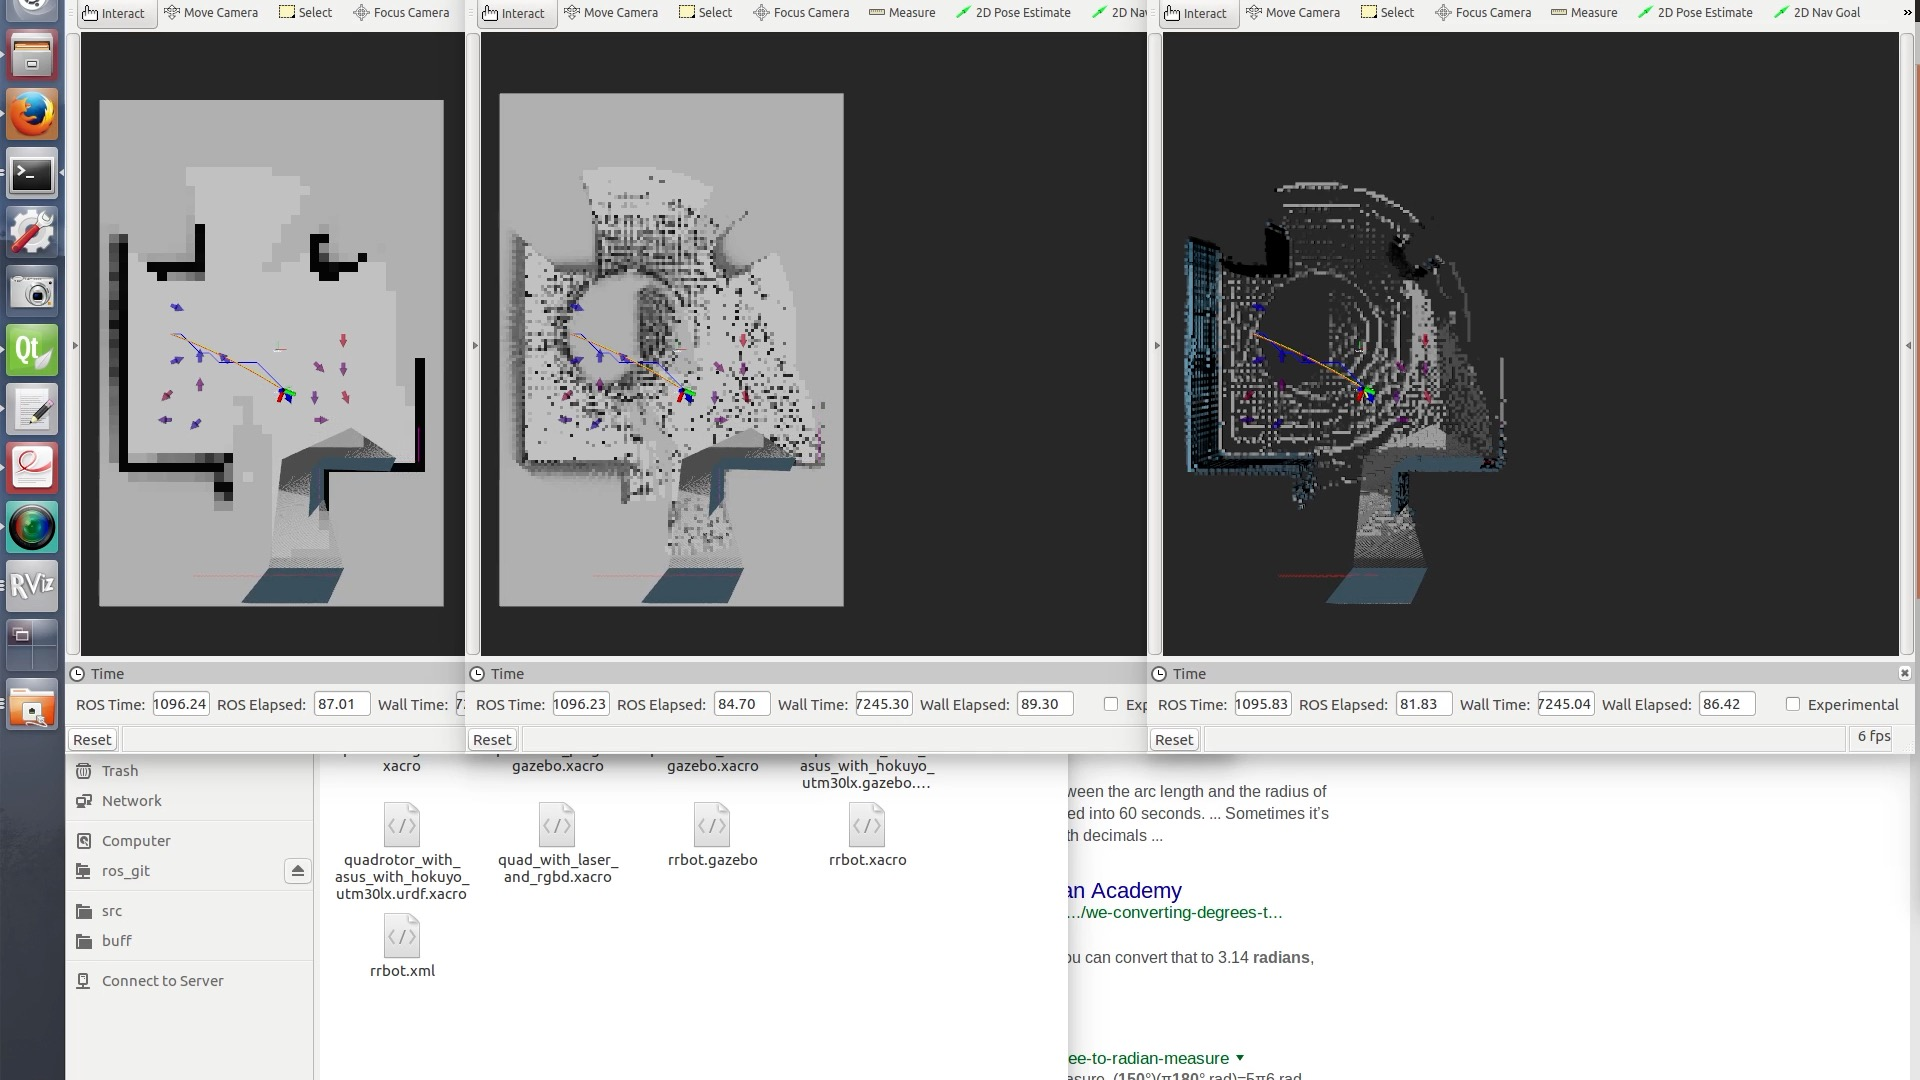
\includegraphics[trim = {41.5cm 17cm 14.3cm 3.8cm}, clip, height=\textwidth]{gazebo_1min.jpg}
        		\caption{$t=1$ min}
    	\end{subfigure}
    	\begin{subfigure}[t]{0.24\columnwidth}
           	\centering
          	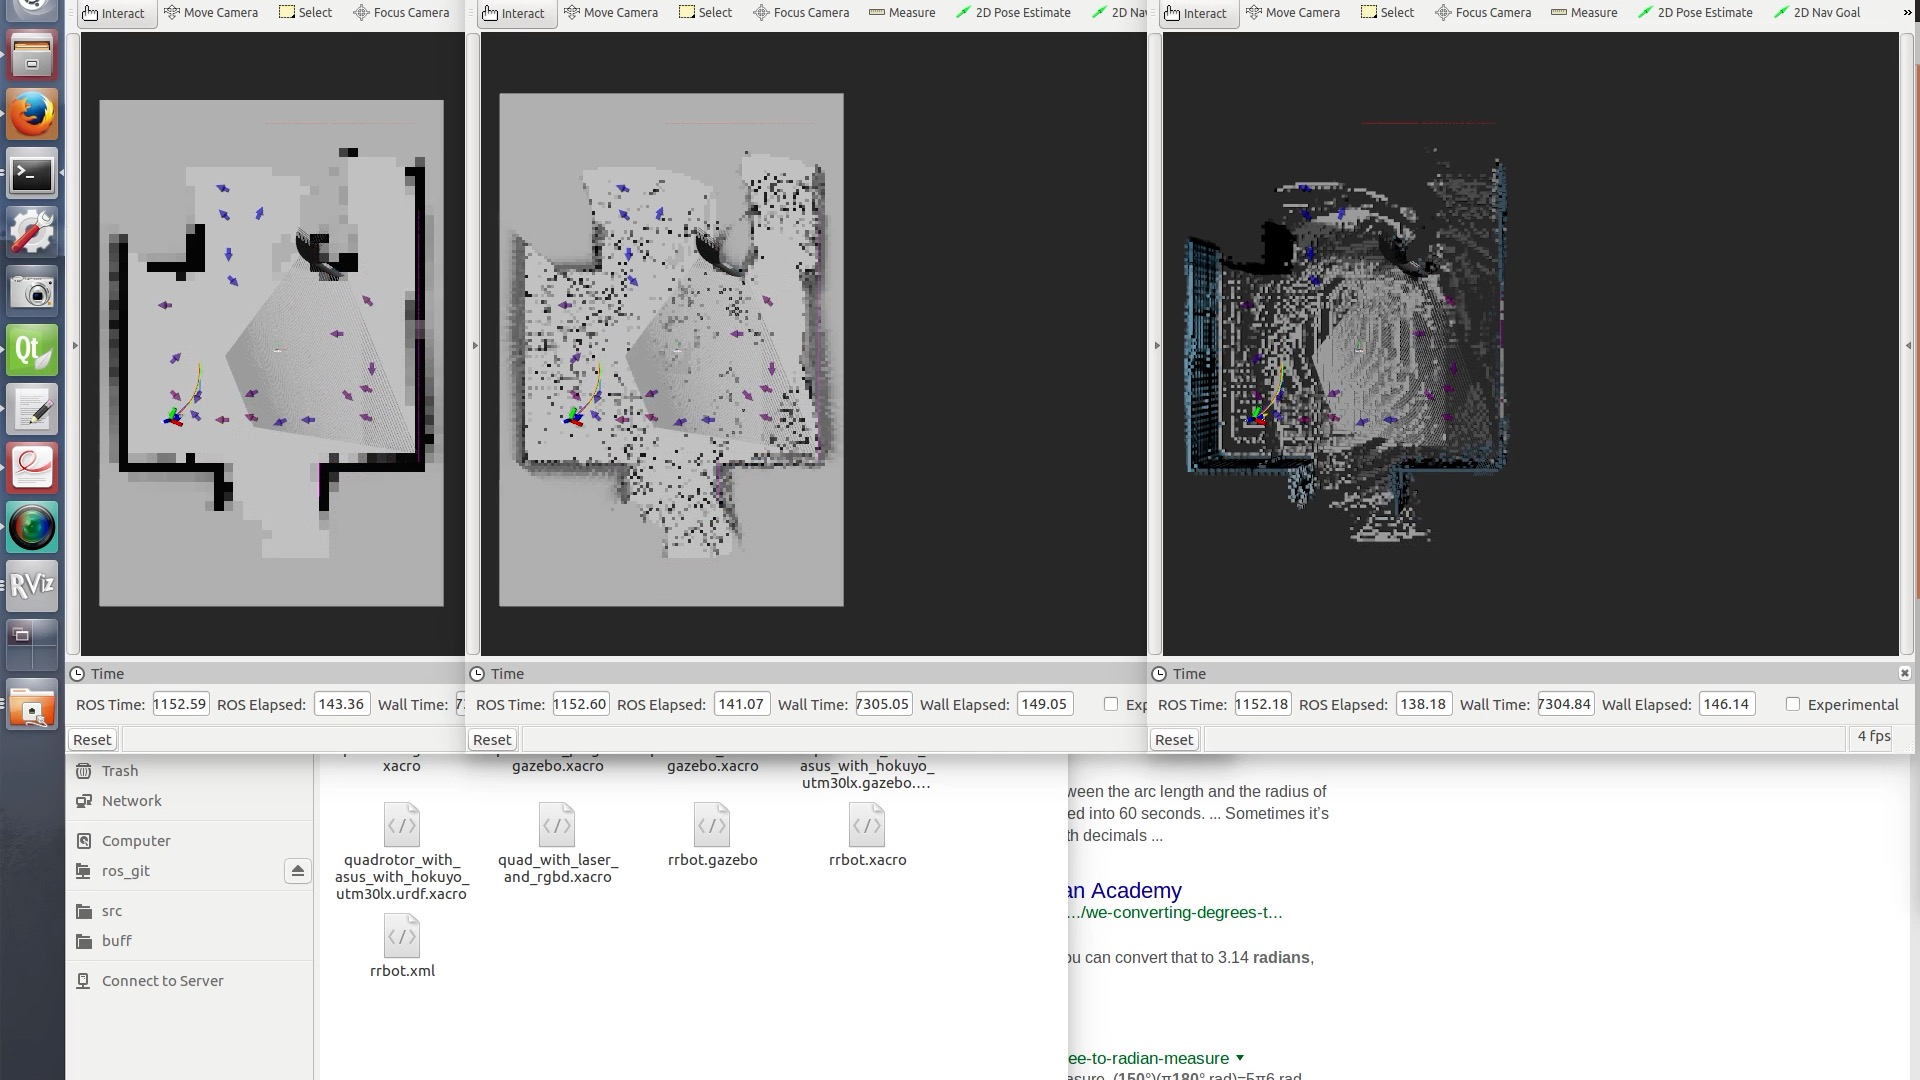
\includegraphics[trim = {41.5cm 17cm 14.3cm 3.8cm}, clip, height=\textwidth]{gazebo_2min.jpg}
        		\caption{$t=2$ min}
    	\end{subfigure}
    	\begin{subfigure}[t]{0.24\columnwidth}
           	\centering
          	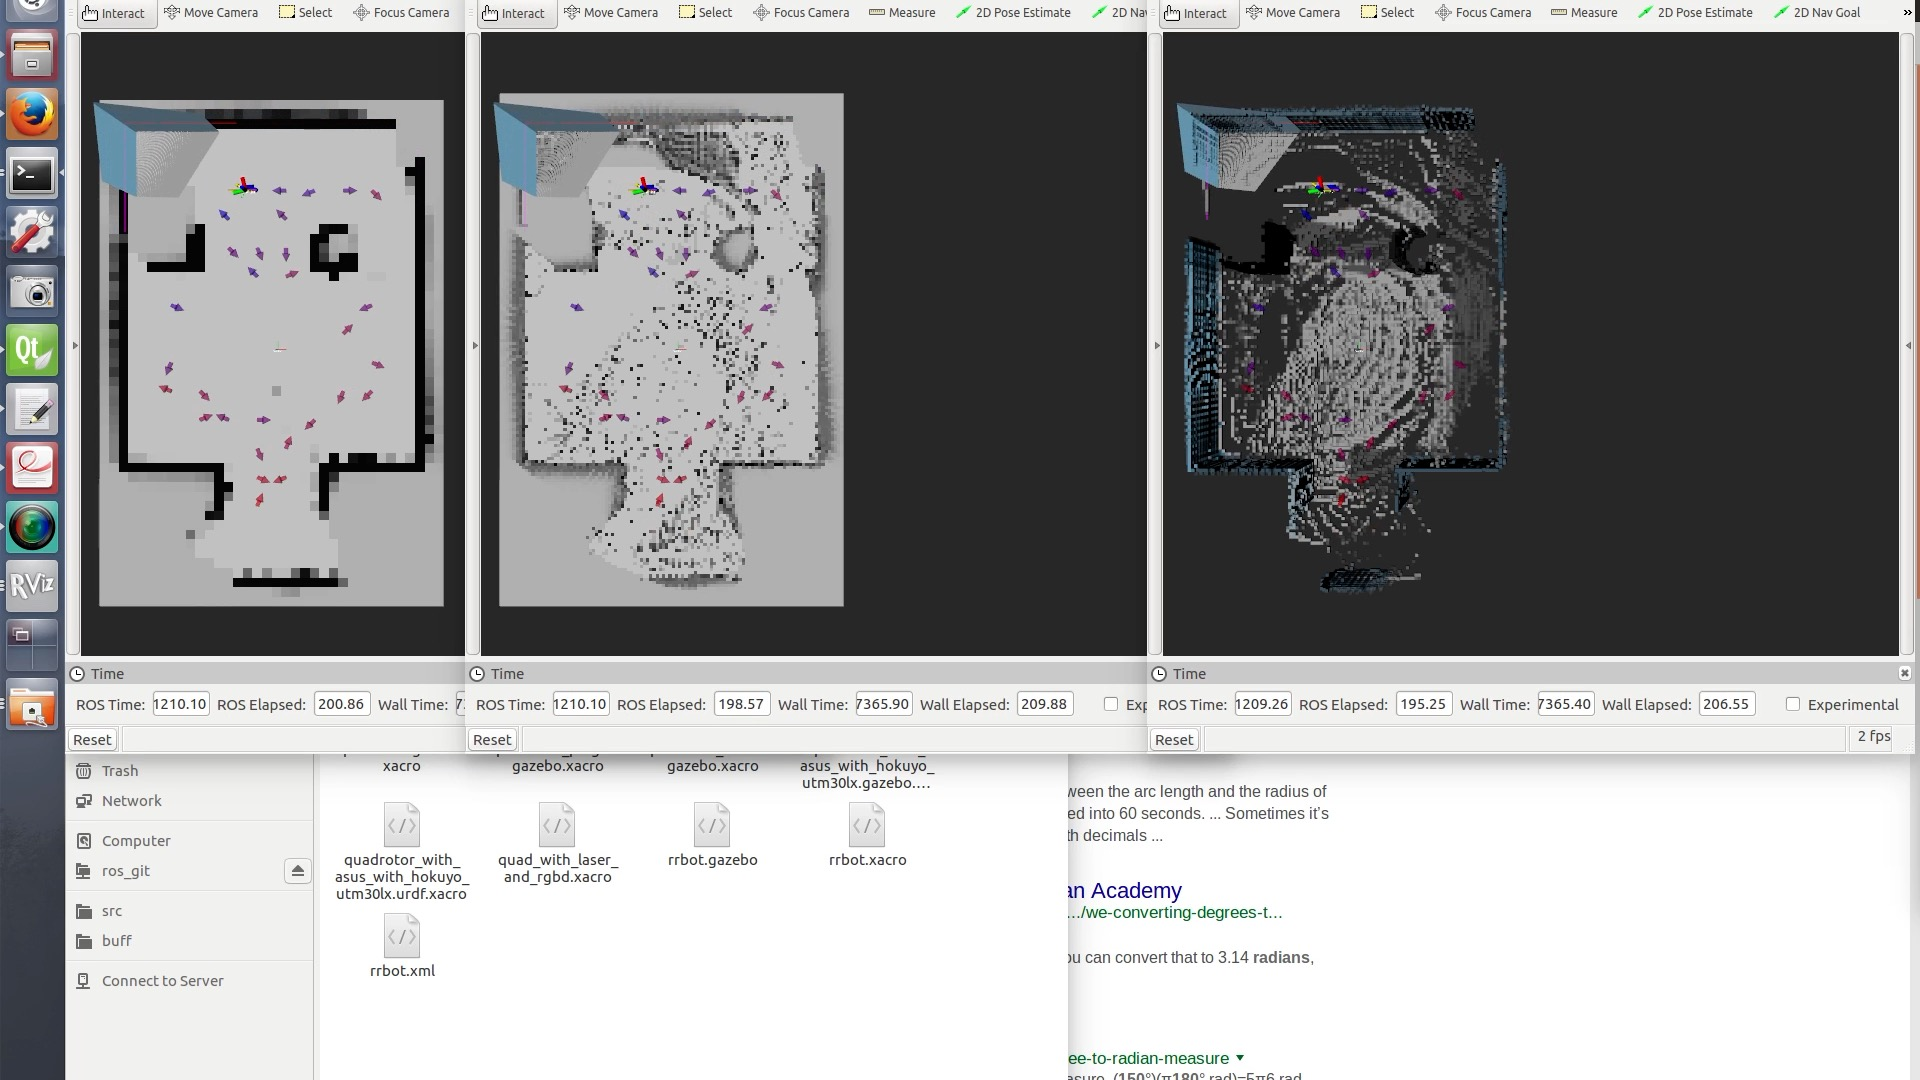
\includegraphics[trim = {41.5cm 17cm 14.3cm 3.8cm}, clip, height=\textwidth]{gazebo_3min.jpg}
        		\caption{$t=3$ min}
   	\end{subfigure}
    	\begin{subfigure}[t]{0.24\columnwidth}
           	\centering
          	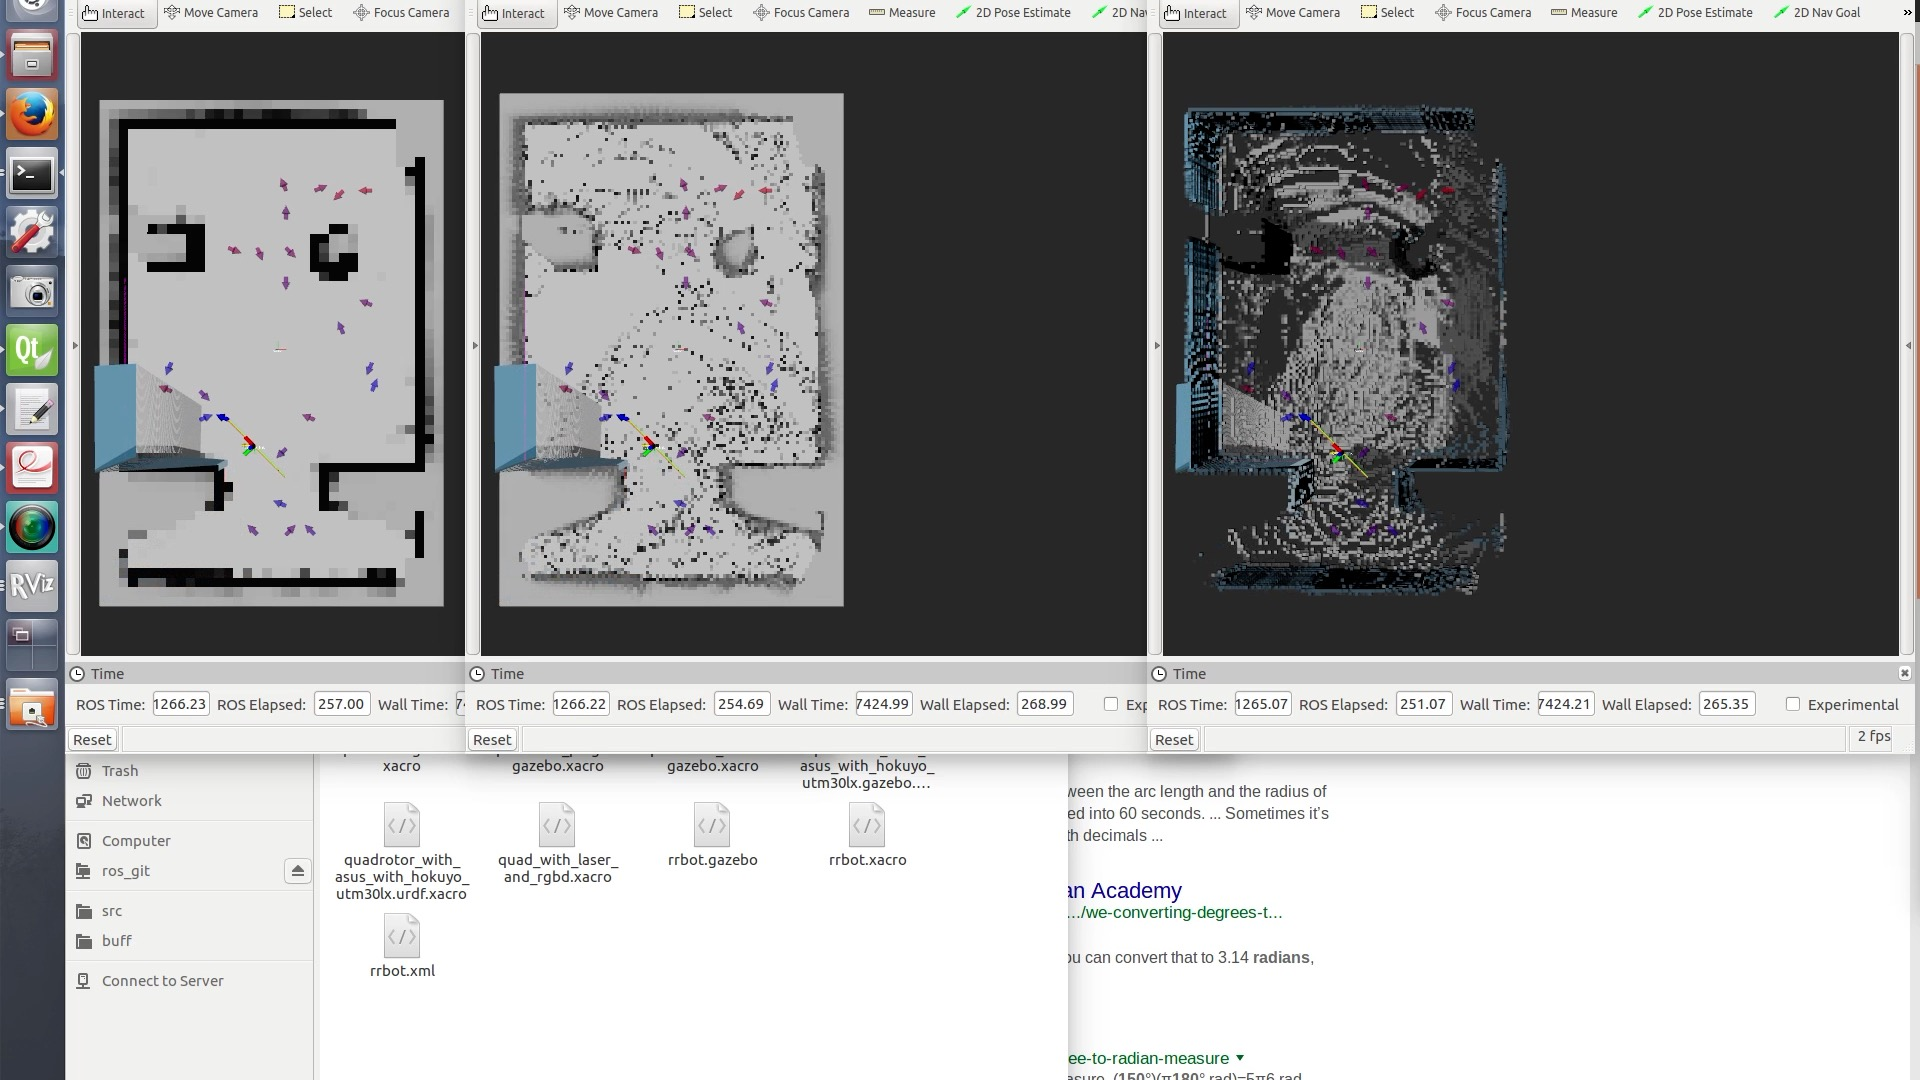
\includegraphics[trim = {41.5cm 17cm 14.3cm 3.8cm}, clip, height=\textwidth]{gazebo_4min.jpg}
        		\caption{$t=4$ min}
    	\end{subfigure}
	\begin{subfigure}[t]{0.24\columnwidth}
	\vspace*{0.15\columnwidth}
           	\centering
          	\includegraphics[trim = {41.5cm 17cm 14.3cm 3.8cm}, clip, height=\textwidth]{gazebo_5min.jpg}
        		\caption{$t=5$ min}
    	\end{subfigure}
    	\begin{subfigure}[t]{0.24\columnwidth}
	\vspace*{0.15\columnwidth}
           	\centering
          	\includegraphics[trim = {41.5cm 17cm 14.3cm 3.8cm}, clip, height=\textwidth]{gazebo_6min.jpg}
        		\caption{$t=6$ min}
    	\end{subfigure}
    	\begin{subfigure}[t]{0.24\columnwidth}
	\vspace*{0.15\columnwidth}
           	\centering
          	\includegraphics[trim = {41.5cm 17cm 14.3cm 3.8cm}, clip, height=\textwidth]{gazebo_7min.jpg}
        		\caption{$t=7$ min}
   	\end{subfigure}
    	\begin{subfigure}[t]{0.24\columnwidth}
	\vspace*{0.15\columnwidth}
           	\centering
          	\includegraphics[trim = {41.5cm 17cm 14.3cm 3.8cm}, clip, height=\textwidth]{gazebo_8min.jpg}
        		\caption{$t=8$ min}
    	\end{subfigure}
%\includegraphics[width=2.5in]{myfigure}
% where an .eps filename suffix will be assumed under latex, 
% and a .pdf suffix will be assumed for pdflatex; or what has been declared
% via \DeclareGraphicsExtensions.
	\caption{Simulated 3D Occupancy Grid Map}
	\medskip
	\small
	A robot (RGB axes) explores a simulated 3D Gazebo environment using separate collision and entropy projected maps. The robot considers numerous candidates (arrows, blue: greater objective function, red: smaller objective function) and selects the optimal candidate (blue arrow).
\label{fig:sim3DMap}
\end{figure}


\begin{figure}
	\centering
	\begin{subfigure}[t]{0.3\columnwidth}
           	\centering
          	\includegraphics[height=1.5\textwidth]{gazebo_view.png}
        		\caption{Environment}
		\label{fig:Sim2ProjMapsGazebo}
    	\end{subfigure}
		\hspace*{0.05cm}
    	\begin{subfigure}[t]{0.3\columnwidth}
           	\centering
          	\includegraphics[trim = {3.6cm 17cm 52.5cm 4cm}, clip, height=1.5\textwidth]{gazebo_4min.jpg}
        		\caption{Collision Map}
		\label{fig:Sim2ProjMapsCollision}
    	\end{subfigure}
	\hspace*{0.1cm}
	\begin{subfigure}[t]{0.3\columnwidth}
           	\centering
          	\includegraphics[trim = {18cm 17cm 38.1cm 4cm}, clip, height=1.5\textwidth]{gazebo_4min.jpg}
        		\caption{Entropy Map}
		\label{fig:Sim2ProjMapsEntropy}
    	\end{subfigure}
%\includegraphics[width=2.5in]{myfigure}
% where an .eps filename suffix will be assumed under latex, 
% and a .pdf suffix will be assumed for pdflatex; or what has been declared
% via \DeclareGraphicsExtensions.
\caption{Simulated Environment and 2D Projected Maps at $4$ min}
	\medskip
	\small
	The robot hovering near the beginning of the simulation is shown in (a). The projected maps for collision (b) and entropy (c) are shown $4$ minutes into the simulation. The robot and candidates are shown the same as Figure \ref{fig:sim3DMap}, where the space is considered mostly collision-free, though still largely uncertain.
\label{fig:sim2Dmaps}
\end{figure}

\begin{figure}[!t]
	\centering
	\includegraphics[width=0.9\textwidth]{entropy_experiment_aspect3by1.pdf}
	\caption{Simulated Environment Map Entropy}
	\medskip
	\small
	The entropy of the full 3D map decreases while the robot follows an autonomous exploration scheme based on projected map cells that consider maximum entropy in the vertical direction.
	\label{fig:simH}
\end{figure}

The two-map approach both exhibits advantages and disadvantages. The exploration algorithm successfully avoided collisions and gave way to a fairly complete 3D occupancy grid. The floor, which is not always visible, is properly estimated in most places. Conversely, this attention to detail has negative consequences that encourage the robot to repeatedly look at the same regions from different vantage points.
Since an entropy map cell is composed from many 3D grid cells single-stacked vertically, if just one of these 3D map cells is not captured or hardly captured, the entropy map cell will be recorded as quite uncertain, shown covering numerous locations in Figure~\ref{fig:Sim2ProjMapsEntropy}. The robot may attempt to measure this space again, even when other regions might more strongly warrant observation. These periods of sluggish entropy decrease are shown with flatter sections of Figure~\ref{fig:simH}. In short, this algorithm successfully explores the space collision-free while producing a complete map, but over-attention to just a few uncertain cells has negative consequences on the exploration speed.






% TODO: move below to experimental results
%\section{Exploring a Large Room}
% IRC18 result: Figure 4, 5, 6, 7


\section{Conclusions}

In this chapter, we proposed an extension of exact probabilistic occupancy grid mapping from 2D to 3D, then proposed a simplified autonomous exploration scheme for vertically-uniform environments. Two versions of the projected map, namely one for collision and one for entropy, are used in a numerical example. The collision and entropy combination map is applied to an experimental result in Chapter \ref{chap:Experiments}.




% !TEX root = ../thesis-sample.tex

\chapter{Autonomous Exploration in Complex 3D Space} \label{chap:ae3Dcomplex}


\section{Exploration with Full 3D Maps}

\subsection{Collision Mapping in 3D}

\subsection{Future Pose Optimization in 3D}

\section{Numerical Simulation}
% Mars simulation

\section{Experiment}
% SEH indoor simulation (needs completing)

\section{Conclusions}






% !TEX root = ../thesis-sample.tex

\chapter{Multi-Vehicle Autonomous Exploration and Patrol} \label{chap:multivehicle}

This chapter covers a bidding-based formulation for multiple vehicles cooperating together in the context of autonomous exploration and patrol. We focus on a series of auctions to assign tasks, and consider dynamic obstacles, such as people, in large office-like environments using a receding-horizon framework.

\section{Bidding-Based Autonomous Exploration}

When exploring uncertain environments, robots can generate large maps much faster if they coordinate their efforts. However, the problem of determining a multi-vehicle exploration strategy is complicated and computationally expensive, but must be performed in real-time.

In this section, we formulate a cooperative and autonomous exploration scheme based on sequential auctions for maximizing map information gain. The first auction is based on the expected information gain presented in the prior section, scaled by travel distance. Once the winner of the first auction is determined, the map for bidding is updated based on the expected measurements of the first robot. The second auction for the remaining robots is determined by the information gain from the revised map that is further scaled by the travel distance and a penalty for collision-avoidance. This process is repeated until all robots are assigned tasks. 

During this chapter, we assume a 3D vertically-uniform environment at a fixed exploration height as described in Chapter \ref{chap:ae3Dsimple} using the 2D projected combination map $m_\text{2D}$. Then information gain is based on \refeqn{ObjFun} and \refeqn{ObjFunApprox}, and depends on this reduced map only, i.e.,
\begin{align}
\label{eqn:expectedInfoGainMap2D}
\mathcal I(X_c,m_\text{2D})&=H(P(m_\text{2D}))-\text{E}\left[H(P(m|X_c,Z_c))\right],
\end{align}
where the expected scan $Z$ is given from \refeqn{expectedInfoGainRay} and \refeqn{FindRc}.


\subsection{Objective Function for the First Auction}


Here, we describe how robots participate in the first auction for maximizing map information gain while accounting for travel time. The information gain \refeqn{ObjFunApproxCompleteCartesian} is computed for each candidate pose. Expected information gains may vary among the robots only if they have different sensor configurations. All expected information gains must be computed prior to the first auction.

Next, we describe how travel time is integrated into exploration. Considering that distances from current robot poses to candidate poses may differ greatly, accounting for these varying travel times properly is essential for exploration time efficiency. Travel distances are computed using Dijkstra's search to provide collision-free waypoints for each robot. There are two steps: first, generate a cost map from the robot location to each location on the 2D projected map. This provides the collision-free distances to all reachable locations on the map, which are different for each robot in general. Second, the waypoints from a candidate pose to the current robot pose are easily obtained along the cost map using steepest descent. 

The travel time is integrated into the autonomous exploration optimization using a bump function similar to \refeqn{BumpFunRef}. Let the distance along the collision-free path from the $k$-th robot pose, namely $X_k$, to the $c$-th candidate pose, namely $X_c$, be denoted $d(X_k,X_c,m_\text{2D})\geq0$, which is taken from the cost map belonging to $X_k$. A continuous bump function is defined to account for traveling costs, and is composed of two parts.  

The first part of the bump function corresponds to short trajectories. Consider $d_\text{opt}$, the time-optimal distance that a robot may travel at full speed during the time between exploration updates. Here, we consider the case when $d(X_k,X_c,m_\text{2D})\leq d_\text{opt}$, i.e., the robot can completely traverse this distance during the allotted travel time. If $d(X_k,X_c,m_\text{2D})\ll d_\text{opt}$, then the robot is not moving at its full potential. This can be wasteful, because the robot tends to capture larger regions while moving. Therefore, it is desirable for $d(X_k,X_c,m_\text{2D})\rightarrow d_\text{opt}$, which corresponds to maximizing map coverage without time cost. The first part of the bump function is sinusoidal and is optimized at $d_\text{opt}$ to maximize robotic movement as
\begin{align}
\label{eqn:BumpFunIncreasing}
\mathcal B_1(d)=\frac12 f_\text{max}\left(1-\cos{\frac{d\pi}{d_\text{opt}}}\right),
\end{align}
where $f_\text{max}>0$ is the maximum value when $d(X_k,X_c,m_\text{2D})=d_\text{opt}$.

The second part of the bump function is defined over the domain where \\$d(X_k,X_c,m_\text{2D})>d_\text{opt}$ to minimize time required for $X_k$ to arrive at $X_c$, putting a penalty on traversing across the environment. This choice is beneficial to generating accurate local maps before exploring new regions. The second half is defined to be nonzero everywhere and is strictly decreasing as 
\begin{align}
\label{eqn:BumpFunDecreasing}
\mathcal B_2(d)=(f_\text{max}-f_\text{far})\exp\braces{-\beta(d_\text{opt}-d)^2}+f_\text{far},
\end{align}
where $f_\text{max}>f_\text{far}>0$ guarantees $\mathcal B_2>0$ such that $\mathcal B_2\rightarrow f_\text{far}$ as $d(X_k,X_c,m_\text{2D})\rightarrow\infty$ and $\beta>0$ assigns the rate of functional decrease relative to $f_\text{max}$ and $f_\text{far}$. Then, the complete bump function is defined as
\begin{align}
\label{eqn:BumpFun}
\mathcal B(d)=
\begin{cases}
    \mathcal B_1(d),		& \text{if }d\leq d_\text{opt},\\
    \mathcal B_2(d),         & \text{otherwise},
\end{cases}
\end{align}
which is illustrated in Fig. \ref{fig:nonzeroBumpFun}. % In short, the bump function prioritizes short movements to capture the local environment over long traversals for exploration time efficiency.

	\begin{figure}
		\centerline{
			\includegraphics[width=0.9\columnwidth]{NonZeroBump.pdf}
		}
		\caption{The bump function is designed to promote travel distances close to $d_\text{opt}$ by multiplying this function by the expected information gain objective. Travel distances less than $d_\text{opt}$ are below the robot capabilities. Travel distances beyond $d_\text{opt}$ are beyond what the robot can reach within the minimum exploration computation time.}
		\label{fig:nonzeroBumpFun}
	\end{figure}
	
Then, using the information gain from \refeqn{expectedInfoGainMap2D} and considering the impact from travel distance from \refeqn{BumpFun}, the objective function for a single agent with respect to $X_{c}$ is
\begin{align}
\label{eqn:CandidateBidSingle}
\text{Obj}_\text{single}(X_k,X_c,m_\text{2D})&=\mathcal B(d(X_k,X_c,m_\text{2D}))\mathcal I(X_{c},m_\text{2D}).
%X_{k,c}^*&=\argmax_{X_c}{\ \mathcal B_{k,c}\mathcal I(X_c)},
\end{align}
Then, the optimal pose selection for the $k$-th agent is
\begin{align}
\label{eqn:OptPoseSingle}
X^*_{k}=\argmax_{X_c}\text{Obj}_\text{single}(X_k,X_c,m_\text{2D}).
\end{align}
Like \refeqn{BumpFunRef}, the bump function from \refeqn{BumpFun} prioritizes robotic movement within the local surrounding space before the robot moves across the map to distant regions, while still considering faraway pose candidates. Unlike \refeqn{BumpFunRef}, \refeqn{BumpFun} discourages the robot from staying motionless or near-motionless.

The first auction includes bids from all robots, and proceeds as follows. Let the set of all $n_R$ robots be denoted $\mathcal R=\braces{R_1,R_2,\dots,R_{n_R}}$ such that the $k$-th robot, namely $R_k$, bids $\text{Obj}_\text{single}(X^*_k,X_c,m_\text{2D})$ from \refeqn{CandidateBidSingle} and \refeqn{OptPoseSingle}. This is repeated for all $k$ such that $R_k\in\mathcal R$. The robot with the largest bid wins the first auction at index $k^*$, and is assigned to travel to $X^*_{k^*}$. Then, the remaining robots must account for the planned trajectory of the robot that won the first auction in subsequent auctions, described next.



\subsection{Objective Function for Subsequent Auctions}

The robots unable to win the first auction are updated to reflect the expected impact of $R_{k^*}$. This robot is expected to modify the probabilistic occupancy grid map, which may significantly change the expected information gains and collision properties of candidate poses nearby $X^*_{k^*}$. The process of auctioning and modifying bids is repeated, removing the winning robot from consideration after each auction, until no robots remain. Between auctions, updating the map with expected measurements from auction-winning robots discourages the remaining robots from entering the same regions and capturing the same cells. As such, there is no need to consider the coverage overlap explicitly: it is avoided in a systematic way as increased coverage overlap would reduce the overall information gain.

More specifically, we coordinate robotic efforts by modifying bids to prevent robots from updating the same grid cells and to avoid collisions among robots. The goal is to find the winning bids $\mathcal X^*=\braces{X^*_{1},X^*_{2},\dots,X^*_{n_R}}$ corresponding to each robot from $\mathcal R$. During the auctioning process, let $\mathcal W\subset\mathcal R$ be the set of robots that have already won auctions by producing the largest objective function bid. After the first auction described above, $\mathcal W=\braces{R_{k^*}}$; after all auctions are complete, $\mathcal W=\mathcal R$. Between auctions, the candidate poses are modified for information gain and collision-avoidance, coordinating the multi-vehicle exploration.

The first step between auctions is to modify the expected map information gain for efficient map coverage.  Once a robot wins a bid, the measurement ray expected values serve to update a temporary copy of $m_\text{2D}$, namely $m_\text{2D,copy}$, and those candidates located in a local neighborhood (twice the radius of a maximum sensor reading) of the winning candidate from the prior auction are recalculated, thereby coordinating total map information gain with auction-winning robots. Using the same local map notation from \refeqn{allEta} and \refeqn{Unnormalized} along a measurement ray, the expected measurement value is
\begin{align}
\label{eqn:ExpectedMeasRay}
\text{E}[z]=\sum_{k=1}^{n_{r}}\bigg\{\prod_{j=0}^{k-1}P(\bar{\mathbf{m}}_j)\bigg\}P(\mathbf{m}_k)z_k,
\end{align}
where $z_k$ denotes the distance from the robot sensor to the $k$-th cell along the measurement ray. Then $\text{E}[z]$ is substituted into \refeqn{RayISMAnswer}--\refeqn{Unnormalized} to modify $m_\text{2D,copy}$, and expected map information gains are recomputed with \refeqn{ProbMeas} and \refeqn{expectedInfoGainRay}, while the bump function \refeqn{BumpFun} remains the same. In short, the expected changes of $m_\text{2D}$ are integrated into $m_\text{2D,copy}$ for expected information gain estimation between multiple vehicles.

The second step focusses on collision-avoidance between robots based on their proximity. Let $\rho_\text{max}>0$ be a fixed maximum radius to consider collision-avoidance and $\rho_{i,c}\geq0$ be the Euclidean distance from the $i$-th already-assigned pose $X^*_i$ to the $c$-th candidate pose $X_c$, i.e.,
\begin{align}
\rho_{i,c}&=\norm{x^*_i-x_c},
\end{align}
where $x^*_i$ and $x_c$ are the pose locations of $X^*_i$ and $X_c$, respectively. Then the collision-avoidance factor for the $k$-th robot such that $R_k\notin\mathcal W$ is,
\begin{align}
\label{eqn:CollisionAvoidanceAmongRobots}
\mathbf C(X_c)&=
\begin{cases}
    \prod_{i|\mathcal{R}_i\in\mathcal W} \left(\frac{\rho_{i,c}}{\rho_\text{max}}\right)^2,		& \text{if }\rho_{i,c}<\rho_\text{max},\\
    1,              				& \text{otherwise},
\end{cases}
\end{align}
where this product serves to decrease the value of bids for candidate poses in close proximity with already-assigned poses to avoid collisions between robots. The multi-vehicle objective function for the $k$-th robot accounting for collision-avoidance is
\begin{align}
\label{eqn:CandidateBidMulti}
\text{Obj}_\text{multi}(X_k,X_c,m_\text{2D,copy})
=\mathbf C(X_c)\mathcal B(d(X_k,X_c,m_\text{2D}))\mathcal I(X_{c},m_\text{2D,copy}),
\end{align}
where its optimal pose during this auction is
\begin{align}
\label{eqn:OptPoseMulti}
X^*_{k}=\argmax_{X_c}\text{Obj}_\text{multi}&(X_k,X_c,m_\text{2D,copy}),
\end{align}
where $\text{Obj}_\text{multi}(X^*_k,X_c,m_\text{2D,copy})$ is the bid for the $k$-th robot.
Optimal pose selection and bidding is repeated for all robots not belonging to $\mathcal W$. The largest bid among these wins the auction and is tasked with moving to the associated pose candidate, and then this robot is included with $\mathcal W$ to avoid further consideration. Completing $n_R$ auctions produces $\mathcal X^*$.

The proposed approach uses auctions and bid modifications based on total map expected information gain and collision-avoidance, promoting exploration of different spaces without explicit consideration of coverage overlaps. The pseudocode for the bidding process is shown with Algorithm \ref{alg:bidding}.

\begin{algorithm}
	Function: $Bidding(\mathcal X_r,\mathcal I(X_c)\forall c\in\mathcal C,\rho_\text{max})$\;
	Initialize $k=0$, $\mathcal W=0_{n_R\times1}$, $B=0_{n_R\times1}$\;
	Update candidate expected information gains using \refeqn{DiscExpEntropyRay}\;
	\For{$i=n_R,n_R-1,\ldots,1$}{
		\For{$j=1,2,\ldots,n_R$}{
			\If{$\mathcal W(j)==0$}{
				\If{$i==n_R$}{
					Maximize bid \refeqn{CandidateBidSingle} for $X^*_{j}$ from \refeqn{OptPoseSingle}\;
				}
				\Else{
					Update $\mathcal I(X_c)$ close to $\mathcal X^*(k)$\;
					\For{$c=1,2,\ldots,n_c$}{
						Find Euclidean distance $\rho_{k,c}$\;
					Get $\mathbf C(X_c)$ with \refeqn{CollisionAvoidanceAmongRobots}\;
					}
					Maximize bid \refeqn{CandidateBidMulti} for $X^*_{j}$ from \refeqn{OptPoseMulti}\;
				}
				Insert the $j$-th maximum bid into $B(j)$\;
			}
		}
		$k$: index maximizing $B$ with corresponding $X^*_{k}$\;
		$\mathcal X^*(k)=X^*_{k}$\;
		$\mathcal W(k)=1$\;
		$B(k)=0$\;
	}

	Return $\mathcal X^*$\;
\caption{Robot Task Bidding}
\label{alg:bidding}
\end{algorithm}


\subsection{Receding Horizon Framework}

\subsection{Multi-Vehicle Exploration Numerical Simulation}
% Multi-vehicle ICRA figs 3-6 (remake fig. 5 with larger contrast)

\section{Multi-Vehicle Cooperative Patrol}

\subsection{Continuous-Time Markov Process for Cell Degradation}
% JINT18 fig. 3

\subsection{Multi-Vehicle Patrol Numerical Simulation}
% JINT18 fig. 10-13 (ref. ICRA fig 3 from above in this chapter)

\section{Conclusions}







\bibliographystyle{plain}
\bibliography{thesis-bib}

% appendices must appear after
% !TEX root = ../thesis-sample.tex
\appendix
\doublespacing
\chapter{Proof of Proposition 1}

\paragraph{Unnormalized Reduced Map Inverse Sensor Model}
For the reduced map of the $l$-th ray, the unnormalized probability that corresponds to the terms without $\eta_{t,l}$ in \refeqn{InvSenModWithProbDens} is given by
\begin{align}
\tilde P&(\mathbf{r}_{l,k}|z_{t,l},X_{1:t},Z_{1:t-1})= \sum_{r\in\mathcal{M}_{k}} p(z_{t,l}|r,X_t) P(r|X_{1:t-1},Z_{1:t-1}).\label{eqn:tildePlk}
\end{align}
Recall $\mathcal{M}_k$ corresponds to the set of maps where the $k$-th cell is occupied. Define a subset $\mathcal{N}_{i,k}\subset \mathcal{M}_k$ for $1\leq i\leq k$ be the set of maps where the $i$-th cell is the first occupied cell. More explicitly, 
\begin{align*}
\mathcal{N}_{i,k} & = \{ r\in\mathcal{M}_k| \mathbf{r}_{l,i+}\}= \{ r\in\mathcal{M}_k| \mathbf{r}_{l,1}=0,\ldots, \mathbf{r}_{l,i-1}=0, \mathbf{r}_{l,i}=1,
\mathbf{r}_{l,k}=1\}.
\end{align*}
Then, $\mathcal{M}_k$ can be written as $\mathcal{M}_k =\bigcup_{i=1}^{k} \mathcal{N}_{i,k}$. Using this, the summation over $\mathcal{M}_k$ at \refeqn{tildePlk} can be decomposed of the summation over each $\mathcal{N}_{i,k}$ to obtain
\begin{align*}
\tilde P(\mathbf{r}_{l,k}|z_{t,l},X_{1:t},Z_{1:t-1})= \sum_{i=1}^k\braces{\sum_{r\in\mathcal{N}_{i,k}} p(z_{t,l}|r,X_t) P(r|X_{1:t-1},Z_{1:t-1})}.
\end{align*}
This is motivated by the fact that the forward sensor model $p(z_{t,l}|r,X_t)$ is identical for all maps in $\mathcal{N}_{i,k}$, such that $p(z_{t,l}|r,X_t)=p(z_{t,l}|\mathbf{r}_{l,i+},X_t)$ and it is moved left of the summation to obtain
\begin{align}
\tilde P(\mathbf{r}_{l,k}|z_{t,l},X_{1:t},Z_{1:t-1})= \sum_{i=1}^k \braces{p(z_{t,l}|\mathbf{r}_{l,i+},X_t) \sum_{r\in\mathcal{N}_{i,k}} P(r|X_{1:t-1},Z_{1:t-1})}.\label{eqn:tildePlk0}
\end{align}
The last term of the above expression corresponds to the a priori probability of $\mathcal{N}_{i,k}$. When $i<k$, it is given by
\begin{align}
\sum_{r\in\mathcal{N}_{i,k}}  &P(r|X_{1:t-1},Z_{1:t-1}) 
\nonumber\\&= \bigg\{\prod_{j=0}^{i-1}P(\bar{\mathbf{r}}_{l,j}|X_{1:t-1},Z_{1:t-1})\bigg\}
P({\mathbf{r}}_{l,i}|X_{1:t-1},Z_{1:t-1})P({\mathbf{r}}_{l,k}|X_{1:t-1},Z_{1:t-1}),\label{eqn:PNik}
\end{align}
and when $i=k$, 
\begin{align}
\sum_{r\in\mathcal{N}_{k,k}} & P(r|X_{1:t-1},Z_{1:t-1})= \bigg\{\prod_{j=0}^{k-1}P(\bar{\mathbf{r}}_{l,j}|X_{1:t-1},Z_{1:t-1})\bigg\}P({\mathbf{r}}_{l,k}|X_{1:t-1},Z_{1:t-1}).\label{eqn:PNkk}
\end{align}
Substituting \refeqn{PNik} and \refeqn{PNkk} into \refeqn{tildePlk0}, we obtain \refeqn{Unnormalized}.



\paragraph{Complement of the Unnormalized Reduced Map Inverse Sensor Model}
An analytic expression for the complement of the unnormalized inverse sensor model is also required  for obtaining the normalizer of the $l$-th ray at time $t$, namely $\eta_{t,l}$. Let $\bar{\mathcal{M}}_k$ be the set of maps where the $k$-th cell is unoccupied, i.e., $\bar{\mathcal{M}}_k = \{ r\in\{0,1\}^{n_{r,l}}\,|\, \mathbf{r}_{l,k}=0\}$. Similar to \refeqn{tildePlk},
\begin{align}
\tilde P&(\bar{\mathbf{r}}_{l,k}|z_{t,l},X_{1:t},Z_{1:t-1})= \sum_{r\in\bar{\mathcal{M}}_{k}} p(z_{t,l}|r,X_t) P(r|X_{1:t-1},Z_{1:t-1}).\label{eqn:tildePbarlk}
\end{align}

Let $\bar{\mathcal{N}}_{i,k}\subset \bar{\mathcal{M}}_k $ for $1\leq i\leq n_{r,l}$ and $i\neq k$ be the set of maps where the $i$-th cell is the first occupied cell. More explicitly, 
\begin{align*}
\bar{\mathcal{N}}_{i,k}=\{r\in\bar{\mathcal{M}}_k\,|\, \mathbf{r}_{l,1}=0,\ldots,\mathbf{r}_{l,i-1}=0,
\mathbf{r}_{l,i}=1,\mathbf{r}_{l,k}=0\}.
\end{align*}
Then, we have $\bar{\mathcal{M}}_k=\bigcup_{\substack{i=1\\i\neq k}}^{n_{r,l}} \bar{\mathcal{N}}_{i,k}$. Note that the forward sensor model $p(z_{t,l}|r,X_t)$ is identical for any maps in $\bar{\mathcal{N}}_{i,k}$, such that $p(z_{t,l}|r,X_t)=p(z_{t,l}|\mathbf{r}_{l,i+},X_t)$. Similar to \refeqn{tildePlk0},
\begin{align}
\tilde P&(\bar{\mathbf{r}}_{l,k}|z_{t,l},X_{1:t},Z_{1:t-1})= \sum_{\substack{i=1\\i\neq k}}^{n_{r,l}} \braces{p(z_{t,l}|\mathbf{r}_{l,i+},X_t) \sum_{r\in\bar{\mathcal{N}}_{i,k}} P(r|X_{1:t-1},Z_{1:t-1})},\label{eqn:tildePbarlk0}
\end{align}
where the last term corresponds to the a priori probability of $\bar{\mathcal{N}}_{i,k}$. When $i<k$, it is given by
\begin{align}
\sum_{r\in\bar{\mathcal{N}}_{i,k}} & P(r|X_{1:t-1},Z_{1:t-1}) \nonumber\\&= \bigg\{\prod_{j=0}^{i-1}P(\bar{\mathbf{r}}_{l,j}|X_{1:t-1},Z_{1:t-1})\bigg\} P({\mathbf{r}}_{l,i}|X_{1:t-1},Z_{1:t-1})P(\bar{\mathbf{r}}_{l,k}|X_{1:t-1},Z_{1:t-1}),\label{eqn:PbarNik1}
\end{align}
and when $k<i$,
\begin{align}
\sum_{r\in\bar{\mathcal{N}}_{i,k}} & P(r|X_{1:t-1},Z_{1:t-1}) = \bigg\{\prod_{j=0}^{i-1}P(\bar{\mathbf{r}}_{l,j}|X_{1:t-1},Z_{1:t-1})\bigg\}
P({\mathbf{r}}_{l,i}|X_{1:t-1},Z_{1:t-1}).\label{eqn:PbarNik2}
\end{align}
Substituting \refeqn{PbarNik1} and \refeqn{PbarNik2} into \refeqn{tildePbarlk0}, we obtain
\begin{align}
\tilde P &(\bar{\mathbf{r}}_k|z_{t,l},X_{1:t},Z_{1:t-1})
=P(\bar{\mathbf{r}}_{l,k}|X_{1:t-1},Z_{1:t-1})\nonumber\\
&\quad\times \bigg[\sum_{i=1}^{k-1}\bigg\{\prod_{j=0}^{i-1}P(\bar{\mathbf{r}}_{l,j}|X_{1:t-1},Z_{1:t-1})\bigg\} p(z_{t,l}|\mathbf{r}_{l,i+},X_t)P(\mathbf{r}_{l,i}|X_{1:t-1},Z_{1:t-1})\bigg]
\nonumber
\\
&\quad
+
\bigg[\sum_{i=k+1}^{n_{r,l}+1}\bigg\{\prod_{j=0}^{i-1}P(\bar{\mathbf{r}}_{l,j}|X_{1:t-1},Z_{1:t-1})\bigg\} p(z_{t,l}|\mathbf{r}_{i+},X_t)P(\mathbf{r}_{l,i}|X_{1:t-1},Z_{1:t-1})\bigg],\label{eqn:tildePbar}
\end{align}
where $p(z_{t,l}|\mathbf{r}_{(n_r+1)+},X_t)$ corresponds to the forward sensor model of maximum reading and $P(\mathbf{r}_{l,n_{r,l}+1}|X_{1:t-1},Z_{1:t-1})=1$ for convenience for the empty map case.

\paragraph{Normalizer}
We have 
\begin{align*}
P(\mathbf{r}_{l,k}|z_{t,l},X_{1:t},Z_{1:t-1})+
P(\bar{\mathbf{r}}_{l,k}|z_{t,l},X_{1:t},Z_{1:t-1})=1.
\end{align*}
Since they share the same normalizer $\eta_{t,l}$, this implies 
\begin{align*}
\eta_{t,l}=[\tilde P(\mathbf{r}_{l,k}|z_{t,l},X_{1:t},Z_{1:t-1})+
\tilde P(\bar{\mathbf{r}}_{l,k}|z_{t,l},X_{1:t},Z_{1:t-1})]^{-1}.
\end{align*}
Substituting \refeqn{Unnormalized} and \refeqn{tildePbar}, and rearranging, we obtain \refeqn{allEta}.






\end{document}
